\documentclass[paper=a4, parskip=half-, ngerman, fontsize=11pt]{scrreprt}
\usepackage[T1]{fontenc}

\usepackage[ngerman]{babel}
\babelprovide[hyphenrules=ngerman-x-latest]{ngerman}

\usepackage{csquotes}
\usepackage[backend=biber]{biblatex}
\addbibresource{Proseminar.bib}

\usepackage{graphicx}
\usepackage{url}
\usepackage{amsmath}
\usepackage{booktabs}
\usepackage{xcolor}

\usepackage{standalone}

% for aligned captions
\usepackage{subcaption}

\usepackage{tikz}
\usetikzlibrary{decorations.markings}
\usepackage[europeanresistors]{circuitikz}
\usetikzlibrary{arrows.meta}
\usetikzlibrary{calc}
\usetikzlibrary{3d}

\usepackage{pgfplots}
\pgfplotsset{compat=1.8}
\usepgfplotslibrary{groupplots}


\begin{document}

% Titelseite
\begin{titlepage}
    \begin{center}
        % Unilogo oben
        
\includegraphics[width=0.5\textwidth]{logo_fernuni_hagen.png}\\[2cm]

        {\LARGE \textbf{Übertragung von Signalen auf elektrischen Leitungen}}\\[2cm]

        \textbf{Proseminar Mathematik in der Technik}\\
        \textbf{Modulnummer:} 61711\\
        Fakultät für Mathematik + Informatik\\[0.5cm]

        \begin{tabbing}
            \hspace{6cm} \= \kill
            \textbf{Name:} \> Sven Schmidt \\
            \textbf{Matrikelnummer:} \> 4125169 \\
            \textbf{Abgabedatum:} \> \today \\
            \textbf{Prüfer:} \> PD Dr.-Ing. Stefan Helfert \\
        \end{tabbing}

        \vfill

        {\large FernUniversität in Hagen}\\
        {\large Sommersemester 2025}
    \end{center}
\end{titlepage}

\chapter{Einführung}
Um elektrische Energie für die verschiedensten Situationen des täglichen Lebens verwenden zu können, muss sie vom
Erzeuger zum Verbraucher --- unter Minimierung von Verlusten --- transportiert werden. Dazu verwendet man elektrische
Leiter, die sich u.a. in ihrer Materialzusammensetzung und geometrischer Anordnung unterscheiden. Es ist daher wichtig
zu verstehen, wie genau der Energietransport in Leitern abläuft. Wir betrachten ausschließlich den Transport
elektrischer Energie auf einfachen Zweidrahtleitern.

Fließt in einem elektrischen Leiter ein Strom, dann bildet sich um ihn herum ein magnetisches Feld aus. Ändert sich der
Strom mit der Zeit, wie es z.B. bei Wechselströmen der Fall ist, dann ändert sich mit ihm das magnetische Feld. Ein
zeitlich variierendes magnetisches Feld verursacht ein elektrisches Feld, das mit dem des Leiters wechselwirkt und
eine  Gegenspannung induziert. Das zwischen zwei Leitern ausgebildete elektrische Feld ändert sich ebenfalls mit dem
zeitlich veränderlichen Strom. Dies führt analog zum Ausbilden eines magnetischen Feldes, welches mit dem des Leiters
wechselwirkt. Die Maxwellsche Theorie beschreibt zeitlich variierende elektrische und magnetische Felder, sogenannte
elektromagnetische Felder. Diese breiten sich als elektromagnetische Wellen in alle Raumrichtungen gleichermaßen aus.
Die Ausbreitung elektromagnetischer Wellen wird mittels elektrischen Leitern so beeinflusst, dass in ihnen elektrische
Energie transportiert werden kann.

Wir betrachten zunächst den einfachsten Fall einer elektromagnetische Wellen als sinusförmige Schwingung fester
Frequenz. Da die Frequenzen der auftretenden Wellen im Bereich 50-60Hz liegen, sind ihre Wellenlängen entsprechend groß
-- sie liegen im Bereich von mehreren Kilometern. Der Querschnitt der betrachteten Leiter ist somit sehr viel kleiner
als die Wellenlängen. Dies führt dazu, dass wir von der Lösung der Maxwellschen Gleichungen absehen können und die
Gleichungen zum Beschreiben elektromagnetischer Wellen in elektrischen Leitern mit der Methode der Ersatzbilder
herleiten können, die sich aus der Anwendung der Kirchhoffschen Regeln ergibt.

Dies führt auf die sogenannten Telegraphenleitungen, die Spannung und Strom entlang eines verlustbehafteten
elektrischen Leiters in Abhängigkeit von Ort und Zeit beschreiben. Dies sind partielle Differentialgleichungen erster
Ordnung, die i.A. nur nummerisch gelöst werden können. Wir betrachten verschiedene vereinfachende Modellannahmen, die
es uns erlauben, die Telegraphenleitungen für diese Spezialfälle analytisch zu lösen, um Aussagen über das qualitative
Verhalten der auftretenden Wellen in Leitern machen zu können. Insbesondere stellt sich heraus, dass sich im
Wesentlichen zwei Wellen im Leitermedium ausbreiten -- eine vorwärts laufende und eine rücklaufende Welle. Letztere
ergibt sich durch Reflektion der vorwärts laufenden Welle am Leiterende. Wir betrachten verschiedene Leiterabschlüsse
und wie sich diese auf die Reflektion der Wellen auswirkt.


\chapter{Modell des Zweidrahtleiters}

In dieser Ausarbeitung beschränken wir uns auf die Untersuchung der Ausbreitung elektromagnetischer Wellen in
Zweidrahtleitern (Paralleldraht), die schematisch in der folgenden Abbildung gezeigt.
\begin{figure}[!h]
    \begin{center}
        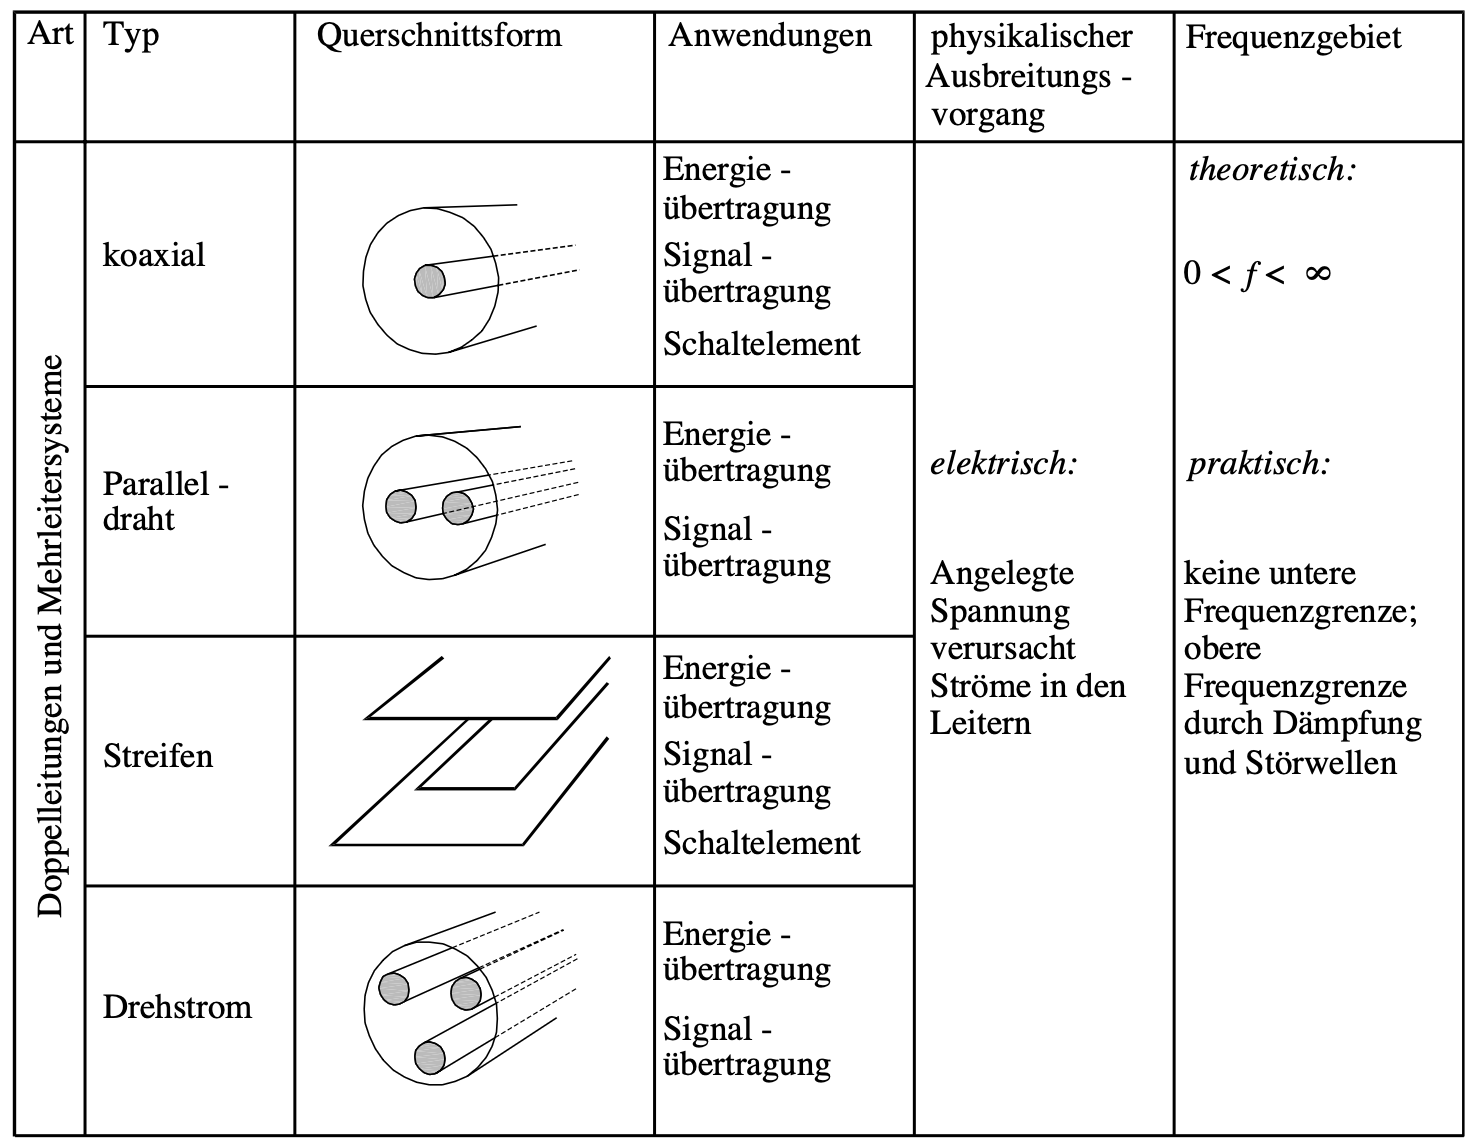
\includegraphics[width=0.5\textwidth]{images/Leiter.png}
        \caption{Elektrische Leiter mit ihren Anwendungen. Entnommen aus~\cite{FernuniSkript}.}
        \label{Leiter}
    \end{center}
\end{figure}

Aus den Gesetzen der Elektro- und Magnetostatik ist bekannt, dass sich beim Durchfließen eines elektrischen Stroms um
einen Leiter ein magnetisches Feld ausbildet (Abbildung~\ref{Felder1}). Variiert dieser Strom zeitlich, dann
verändert sich mit ihm das magnetische Feld und dies wiederum bewirkt die Ausbildung eines elektrischen Feldes, welches
sich als induzierte Gegenspannung bemerkbar macht.
\begin{figure}[!ht]
%    \centering
    \begin{subfigure}[b]{0.49\textwidth}
        \centering
        \documentclass{standalone}

\usepackage{tikz}
\usetikzlibrary{decorations.markings}
\usetikzlibrary{arrows.meta}
\usetikzlibrary{calc}

\usepackage{amsmath}

\begin{document}


\begin{tikzpicture}

% Define styles
\tikzset{
    charge/.style={fill=orange!10, draw=orange, circle, radius=0.4},
    fieldline/.style={thick, postaction={decorate}, decoration={markings}},
    arrow/.style={decoration={mark=at position #1 with {\arrow{Stealth}}}},
    reversearrow/.style={decoration={mark=at position #1 with {\arrowreversed{Stealth}}}}
}

% grind lines
\draw[help lines, dashed] grid (10,10);

%position of bottom wire
\coordinate (A1) at (5,3);

%position of top wire
\coordinate (A2) at (5,7);

% Negative charge node
\draw[charge] (A1) circle node[below=0.2cm] {$-i$};
\node[circle, fill=black, inner sep=2pt] at (A1) {};

% Positive charge node
\draw[charge] (A2) circle node[above=0.2cm] {$+i$};
\node at (A2) {\Large$\boldsymbol{\times}$};

% Magnetic field lines
\draw[fieldline, reversearrow=0.5] (2,8.5) arc (-180:0:3cm and 3cm);

% Magnetic field lines
\draw[fieldline, reversearrow=0.5] (2,8.5) arc (-180:0:3cm and 3cm);
\draw[fieldline, reversearrow=0.75] (5,7) circle[radius=0.9];
\draw[fieldline, arrow=0.5] (8,5) -- (2,5);
\draw[fieldline, reversearrow=0.5] (2,1.5) arc (180:0:3cm and 3cm);
\draw[fieldline, arrow=0.25] (5,3) circle[radius=0.9];

% Magnetic field label
\node at ($(A2)+(45:1.5)$) {\textbf{H}};

\end{tikzpicture}


\end{document}
        \caption{\color{red}Caption for the first picture}
        \label{Felder1}
    \end{subfigure}%
    \hfill
    \begin{subfigure}[b]{0.49\textwidth}
        \centering
        \documentclass[paper=a4, parskip=half-, ngerman, fontsize=11pt]{scrreprt}
\usepackage[T1]{fontenc}

\usepackage[ngerman]{babel}
\babelprovide[hyphenrules=ngerman-x-latest]{ngerman}

\usepackage{csquotes}
\usepackage[backend=biber]{biblatex}
\addbibresource{Proseminar.bib}

\usepackage{graphicx}
\usepackage{url}
\usepackage{amsmath}
\usepackage{booktabs}
\usepackage{xcolor}
\usepackage{standalone}

% for aligned captions
\usepackage{subcaption}

\usepackage{tikz}
\usetikzlibrary{decorations.markings}
\usetikzlibrary{arrows.meta}
\usetikzlibrary{calc}


\begin{document}

% Titelseite
\begin{titlepage}
    \begin{center}
        % Unilogo oben
        
\includegraphics[width=0.5\textwidth]{logo_fernuni_hagen.png}\\[2cm]

        {\LARGE \textbf{Übertragung von Signalen auf elektrischen Leitungen}}\\[2cm]

        \textbf{Proseminar Mathematik in der Technik}\\
        \textbf{Modulnummer:} 61711\\
        Fakultät für Mathematik + Informatik\\[0.5cm]

        \begin{tabbing}
            \hspace{6cm} \= \kill
            \textbf{Name:} \> Sven Schmidt \\
            \textbf{Matrikelnummer:} \> 4125169 \\
            \textbf{Abgabedatum:} \> \today \\
            \textbf{Prüfer:} \> PD Dr.-Ing. Stefan Helfert \\
        \end{tabbing}

        \vfill

        {\large FernUniversität in Hagen}\\
        {\large Sommersemester 2025}
    \end{center}
\end{titlepage}

\chapter{Einführung}

\chapter{Modell des Zweidrahtleiters}

In dieser Ausarbeitung beschränken wir uns auf die Untersuchung der Ausbreitung elektromagnetischer Wellen in
Zweidrahtleitern (Paralleldraht), die schematisch in der folgenden Abbildung gezeigt.
\begin{figure}[!h]
    \begin{center}
        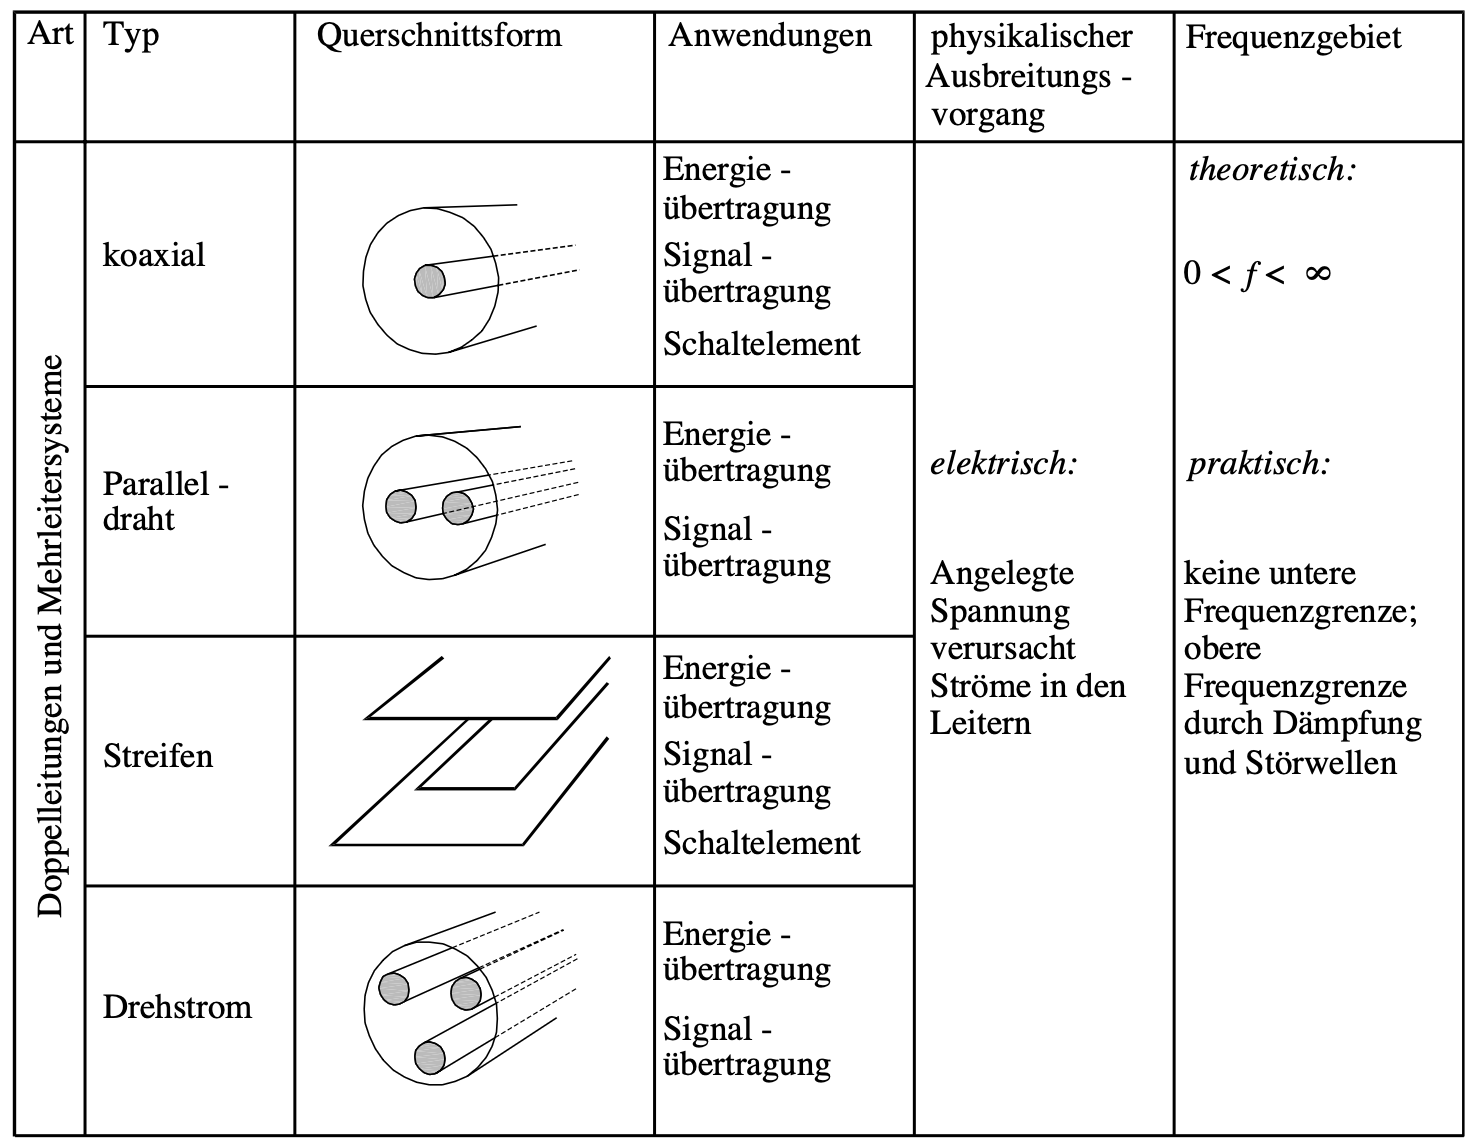
\includegraphics[width=0.5\textwidth]{images/Leiter.png}
        \caption{Elektrische Leiter mit ihren Anwendungen. Entnommen aus~\cite{FernuniSkript}.}
        \label{Leiter}
    \end{center}
\end{figure}

Aus den Gesetzen der Elektro- und Magnetostatik ist bekannt, dass sich beim Durchfließen eines elektrischen Stroms um
einen Leiter ein magnetisches Feld ausbildet (Abbildung~\ref{Felder1}). Variiert dieser Strom zeitlich, dann
verändert sich mit ihm das magnetische Feld und dies wiederum bewirkt die Ausbildung eines elektrischen Feldes, welches
sich als induzierte Gegenspannung bemerkbar macht.
\begin{figure}[!ht]
%    \centering
    \begin{subfigure}[b]{0.5\textwidth}
        \centering
%        \documentclass{standalone}

\usepackage{tikz}
\usetikzlibrary{decorations.markings}
\usetikzlibrary{arrows.meta}
\usetikzlibrary{calc}

\usepackage{amsmath}

\begin{document}


\begin{tikzpicture}

% Define styles
\tikzset{
    charge/.style={fill=orange!10, draw=orange, circle, radius=0.4},
    fieldline/.style={thick, postaction={decorate}, decoration={markings}},
    arrow/.style={decoration={mark=at position #1 with {\arrow{Stealth}}}},
    reversearrow/.style={decoration={mark=at position #1 with {\arrowreversed{Stealth}}}}
}

% grind lines
\draw[help lines, dashed] grid (10,10);

%position of bottom wire
\coordinate (A1) at (5,3);

%position of top wire
\coordinate (A2) at (5,7);

% Negative charge node
\draw[charge] (A1) circle node[below=0.2cm] {$-i$};
\node[circle, fill=black, inner sep=2pt] at (A1) {};

% Positive charge node
\draw[charge] (A2) circle node[above=0.2cm] {$+i$};
\node at (A2) {\Large$\boldsymbol{\times}$};

% Magnetic field lines
\draw[fieldline, reversearrow=0.5] (2,8.5) arc (-180:0:3cm and 3cm);

% Magnetic field lines
\draw[fieldline, reversearrow=0.5] (2,8.5) arc (-180:0:3cm and 3cm);
\draw[fieldline, reversearrow=0.75] (5,7) circle[radius=0.9];
\draw[fieldline, arrow=0.5] (8,5) -- (2,5);
\draw[fieldline, reversearrow=0.5] (2,1.5) arc (180:0:3cm and 3cm);
\draw[fieldline, arrow=0.25] (5,3) circle[radius=0.9];

% Magnetic field label
\node at ($(A2)+(45:1.5)$) {\textbf{H}};

\end{tikzpicture}


\end{document}
        \includegraphics[width=0.6\linewidth]{../graphics/MagnetischeFeldlinien/document}
        \caption{\color{red}Caption for the first picture}
        \label{Felder1}
    \end{subfigure}%
    \hfill
    \begin{subfigure}[b]{0.45\textwidth}
        \centering
%        \documentclass[paper=a4, parskip=half-, ngerman, fontsize=11pt]{scrreprt}
\usepackage[T1]{fontenc}

\usepackage[ngerman]{babel}
\babelprovide[hyphenrules=ngerman-x-latest]{ngerman}

\usepackage{csquotes}
\usepackage[backend=biber]{biblatex}
\addbibresource{Proseminar.bib}

\usepackage{graphicx}
\usepackage{url}
\usepackage{amsmath}
\usepackage{booktabs}
\usepackage{xcolor}
\usepackage{standalone}

% for aligned captions
\usepackage{subcaption}

\usepackage{tikz}
\usetikzlibrary{decorations.markings}
\usetikzlibrary{arrows.meta}
\usetikzlibrary{calc}


\begin{document}

% Titelseite
\begin{titlepage}
    \begin{center}
        % Unilogo oben
        
\includegraphics[width=0.5\textwidth]{logo_fernuni_hagen.png}\\[2cm]

        {\LARGE \textbf{Übertragung von Signalen auf elektrischen Leitungen}}\\[2cm]

        \textbf{Proseminar Mathematik in der Technik}\\
        \textbf{Modulnummer:} 61711\\
        Fakultät für Mathematik + Informatik\\[0.5cm]

        \begin{tabbing}
            \hspace{6cm} \= \kill
            \textbf{Name:} \> Sven Schmidt \\
            \textbf{Matrikelnummer:} \> 4125169 \\
            \textbf{Abgabedatum:} \> \today \\
            \textbf{Prüfer:} \> PD Dr.-Ing. Stefan Helfert \\
        \end{tabbing}

        \vfill

        {\large FernUniversität in Hagen}\\
        {\large Sommersemester 2025}
    \end{center}
\end{titlepage}

\chapter{Einführung}

\chapter{Modell des Zweidrahtleiters}

In dieser Ausarbeitung beschränken wir uns auf die Untersuchung der Ausbreitung elektromagnetischer Wellen in
Zweidrahtleitern (Paralleldraht), die schematisch in der folgenden Abbildung gezeigt.
\begin{figure}[!h]
    \begin{center}
        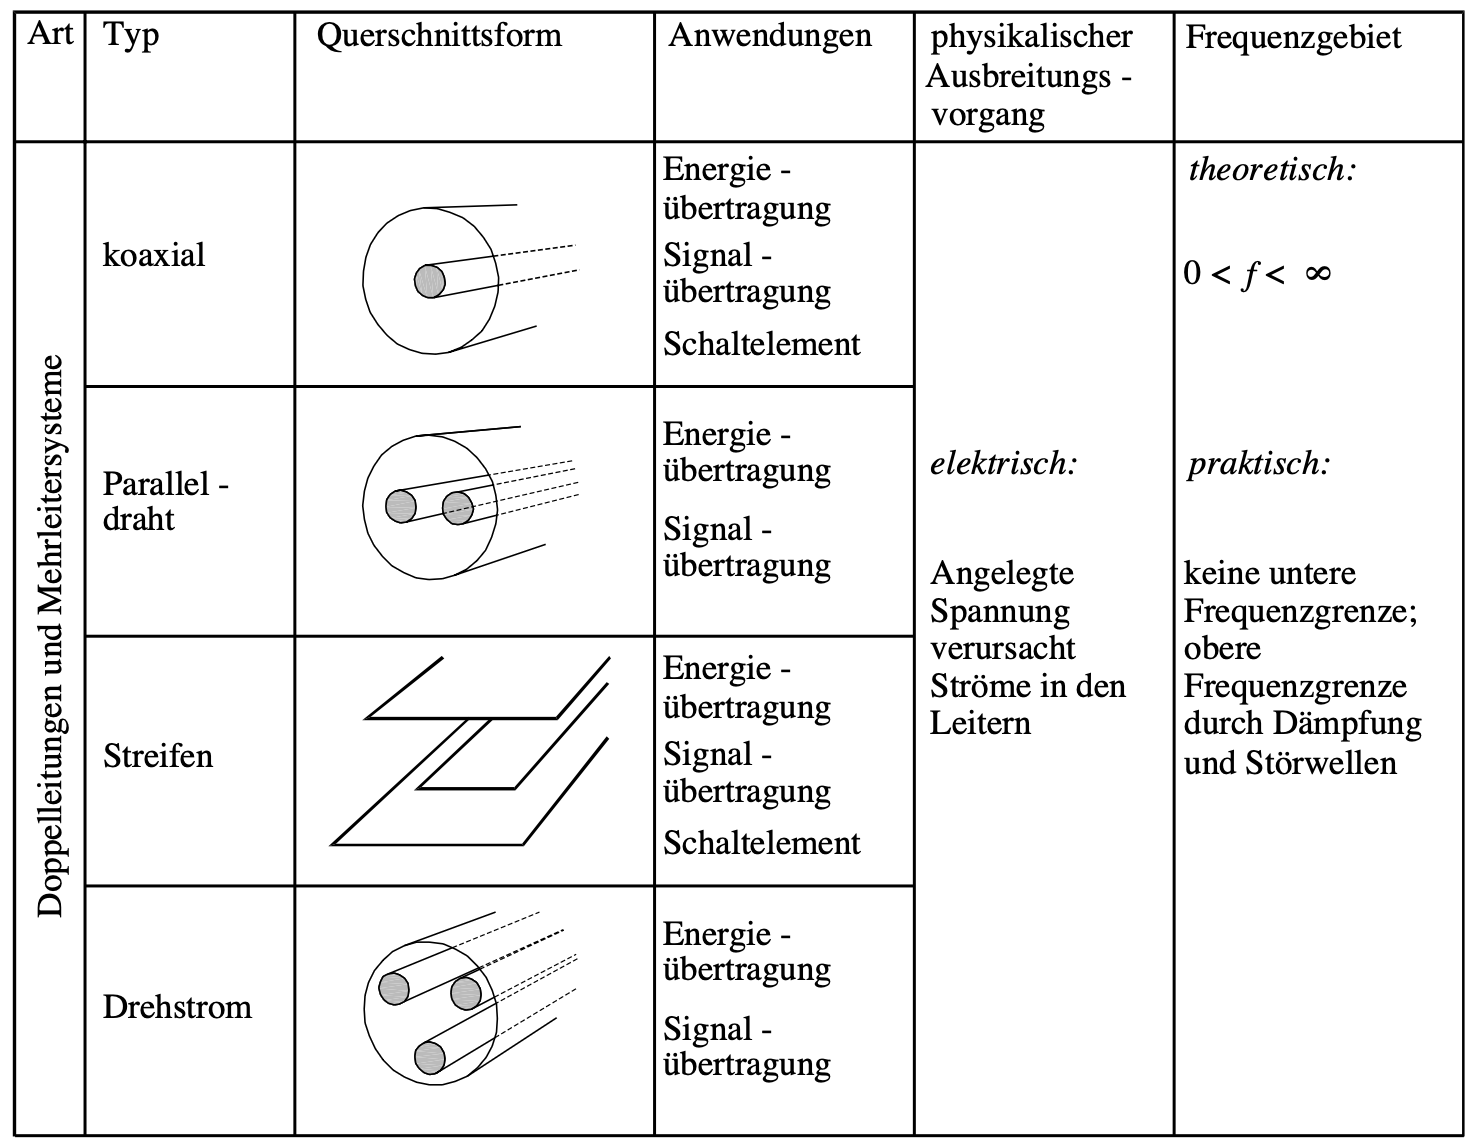
\includegraphics[width=0.5\textwidth]{images/Leiter.png}
        \caption{Elektrische Leiter mit ihren Anwendungen. Entnommen aus~\cite{FernuniSkript}.}
        \label{Leiter}
    \end{center}
\end{figure}

Aus den Gesetzen der Elektro- und Magnetostatik ist bekannt, dass sich beim Durchfließen eines elektrischen Stroms um
einen Leiter ein magnetisches Feld ausbildet (Abbildung~\ref{Felder1}). Variiert dieser Strom zeitlich, dann
verändert sich mit ihm das magnetische Feld und dies wiederum bewirkt die Ausbildung eines elektrischen Feldes, welches
sich als induzierte Gegenspannung bemerkbar macht.
\begin{figure}[!ht]
%    \centering
    \begin{subfigure}[b]{0.5\textwidth}
        \centering
%        \documentclass{standalone}

\usepackage{tikz}
\usetikzlibrary{decorations.markings}
\usetikzlibrary{arrows.meta}
\usetikzlibrary{calc}

\usepackage{amsmath}

\begin{document}


\begin{tikzpicture}

% Define styles
\tikzset{
    charge/.style={fill=orange!10, draw=orange, circle, radius=0.4},
    fieldline/.style={thick, postaction={decorate}, decoration={markings}},
    arrow/.style={decoration={mark=at position #1 with {\arrow{Stealth}}}},
    reversearrow/.style={decoration={mark=at position #1 with {\arrowreversed{Stealth}}}}
}

% grind lines
\draw[help lines, dashed] grid (10,10);

%position of bottom wire
\coordinate (A1) at (5,3);

%position of top wire
\coordinate (A2) at (5,7);

% Negative charge node
\draw[charge] (A1) circle node[below=0.2cm] {$-i$};
\node[circle, fill=black, inner sep=2pt] at (A1) {};

% Positive charge node
\draw[charge] (A2) circle node[above=0.2cm] {$+i$};
\node at (A2) {\Large$\boldsymbol{\times}$};

% Magnetic field lines
\draw[fieldline, reversearrow=0.5] (2,8.5) arc (-180:0:3cm and 3cm);

% Magnetic field lines
\draw[fieldline, reversearrow=0.5] (2,8.5) arc (-180:0:3cm and 3cm);
\draw[fieldline, reversearrow=0.75] (5,7) circle[radius=0.9];
\draw[fieldline, arrow=0.5] (8,5) -- (2,5);
\draw[fieldline, reversearrow=0.5] (2,1.5) arc (180:0:3cm and 3cm);
\draw[fieldline, arrow=0.25] (5,3) circle[radius=0.9];

% Magnetic field label
\node at ($(A2)+(45:1.5)$) {\textbf{H}};

\end{tikzpicture}


\end{document}
        \includegraphics[width=0.6\linewidth]{../graphics/MagnetischeFeldlinien/document}
        \caption{\color{red}Caption for the first picture}
        \label{Felder1}
    \end{subfigure}%
    \hfill
    \begin{subfigure}[b]{0.45\textwidth}
        \centering
%        \documentclass[paper=a4, parskip=half-, ngerman, fontsize=11pt]{scrreprt}
\usepackage[T1]{fontenc}

\usepackage[ngerman]{babel}
\babelprovide[hyphenrules=ngerman-x-latest]{ngerman}

\usepackage{csquotes}
\usepackage[backend=biber]{biblatex}
\addbibresource{Proseminar.bib}

\usepackage{graphicx}
\usepackage{url}
\usepackage{amsmath}
\usepackage{booktabs}
\usepackage{xcolor}
\usepackage{standalone}

% for aligned captions
\usepackage{subcaption}

\usepackage{tikz}
\usetikzlibrary{decorations.markings}
\usetikzlibrary{arrows.meta}
\usetikzlibrary{calc}


\begin{document}

% Titelseite
\begin{titlepage}
    \begin{center}
        % Unilogo oben
        
\includegraphics[width=0.5\textwidth]{logo_fernuni_hagen.png}\\[2cm]

        {\LARGE \textbf{Übertragung von Signalen auf elektrischen Leitungen}}\\[2cm]

        \textbf{Proseminar Mathematik in der Technik}\\
        \textbf{Modulnummer:} 61711\\
        Fakultät für Mathematik + Informatik\\[0.5cm]

        \begin{tabbing}
            \hspace{6cm} \= \kill
            \textbf{Name:} \> Sven Schmidt \\
            \textbf{Matrikelnummer:} \> 4125169 \\
            \textbf{Abgabedatum:} \> \today \\
            \textbf{Prüfer:} \> PD Dr.-Ing. Stefan Helfert \\
        \end{tabbing}

        \vfill

        {\large FernUniversität in Hagen}\\
        {\large Sommersemester 2025}
    \end{center}
\end{titlepage}

\chapter{Einführung}

\chapter{Modell des Zweidrahtleiters}

In dieser Ausarbeitung beschränken wir uns auf die Untersuchung der Ausbreitung elektromagnetischer Wellen in
Zweidrahtleitern (Paralleldraht), die schematisch in der folgenden Abbildung gezeigt.
\begin{figure}[!h]
    \begin{center}
        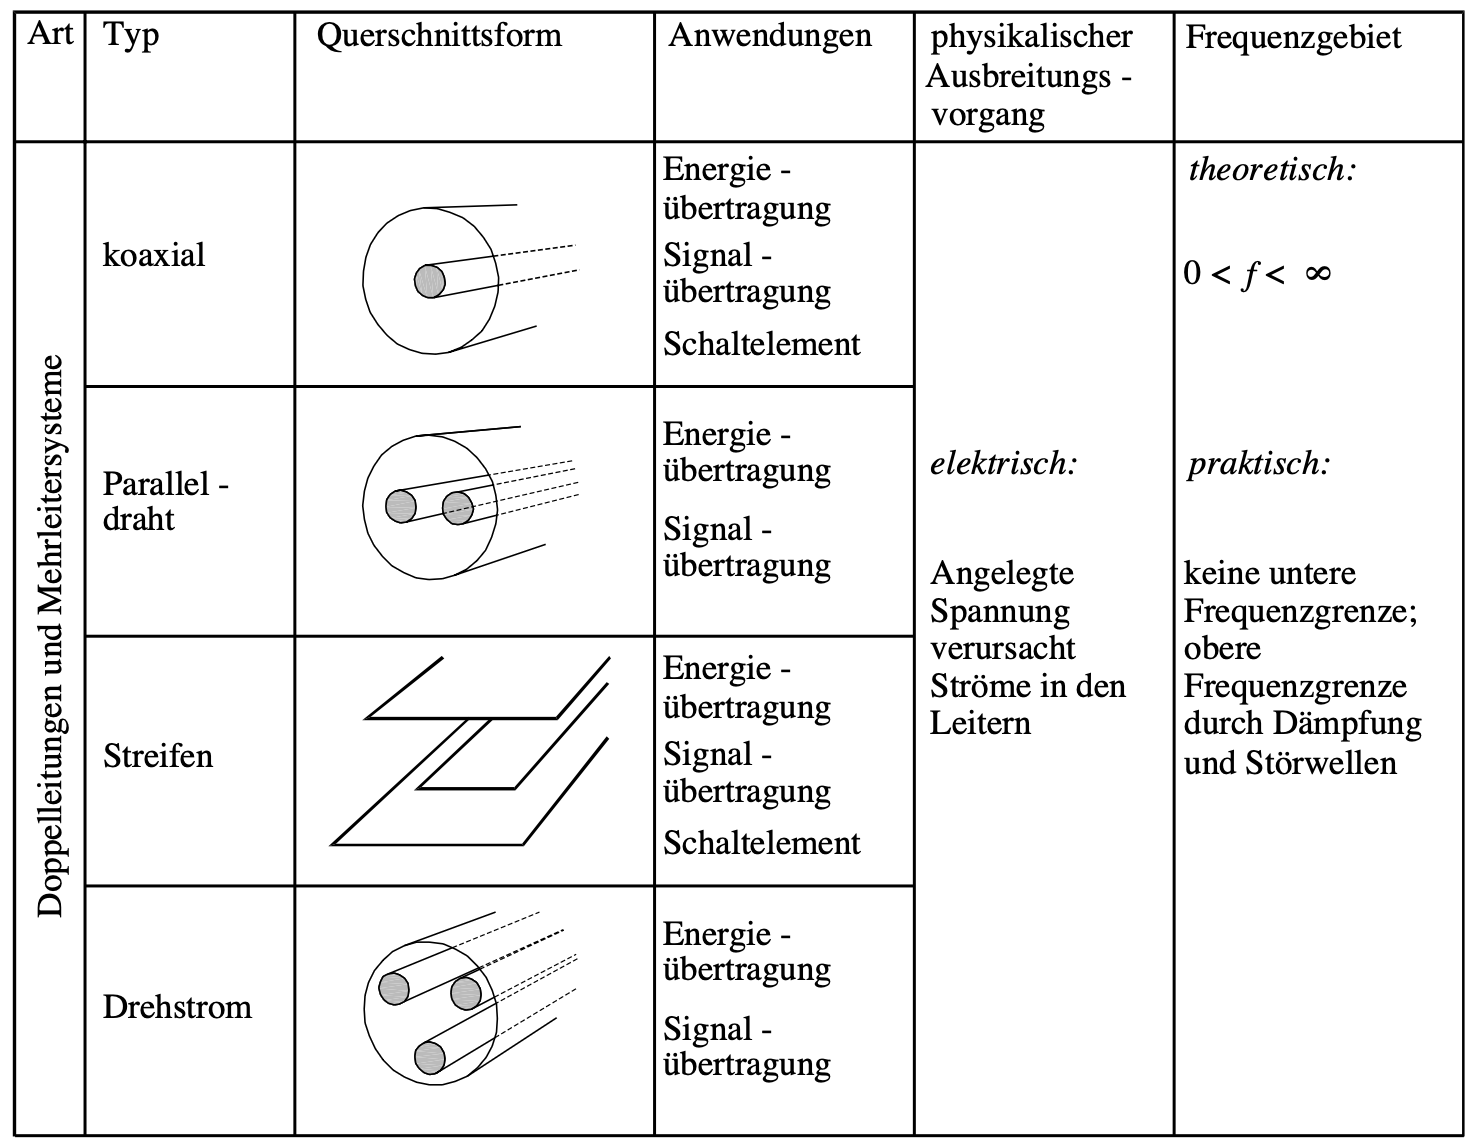
\includegraphics[width=0.5\textwidth]{images/Leiter.png}
        \caption{Elektrische Leiter mit ihren Anwendungen. Entnommen aus~\cite{FernuniSkript}.}
        \label{Leiter}
    \end{center}
\end{figure}

Aus den Gesetzen der Elektro- und Magnetostatik ist bekannt, dass sich beim Durchfließen eines elektrischen Stroms um
einen Leiter ein magnetisches Feld ausbildet (Abbildung~\ref{Felder1}). Variiert dieser Strom zeitlich, dann
verändert sich mit ihm das magnetische Feld und dies wiederum bewirkt die Ausbildung eines elektrischen Feldes, welches
sich als induzierte Gegenspannung bemerkbar macht.
\begin{figure}[!ht]
%    \centering
    \begin{subfigure}[b]{0.5\textwidth}
        \centering
%        \input{../graphics/MagnetischeFeldlinien/document}
        \includegraphics[width=0.6\linewidth]{../graphics/MagnetischeFeldlinien/document}
        \caption{\color{red}Caption for the first picture}
        \label{Felder1}
    \end{subfigure}%
    \hfill
    \begin{subfigure}[b]{0.45\textwidth}
        \centering
%        \input{../graphics/ElektrischeFeldlinien/document}
        \includegraphics[width=0.9\linewidth]{../graphics/ElektrischeFeldlinien/document}
        \caption{\color{red}Caption for the second picture}
        \label{Felder2}
    \end{subfigure}
    \caption{\color{red}Overall caption for the figure}
\end{figure}
Analog geht mit einer an den Leitern anliegende Spannung ein elektrischen Feld einher (Abbildung~\ref{Felder2}).
Ändert sich dieses, so hat dies die Ausbildung eines magnetischen Feldes zur Folge, welches mit dem des Stroms
wechselwirkt.


Im Folgenden nehmen wir an, dass der Leiter parallel verläuft, der Abstand $d$ zwischen den Leitern und der Querschnitt
des Leiters viel kleiner ist, als die Wellenlänge $\lambda$ der auftretenden Signale,
\[ d \ll \lambda = \frac{c_{0}}{f \sqrt{\epsilon_{r}}}. \]
In diesem Fall müssen wir nicht die Maxwellschen Gleichungen
lösen -- statt dessen können wir mit der Methode der Ersatzschaltbilder die Signalübertragung direkt mit den
beteiligten Strömen und Spannungen beschreiben, ohne mit den elektrischen und magnetischen Feldern
argumentieren zu müssen.

Es ist $c_{0}$ die Lichtgeschwindigkeit im Vakuum, $f$ die Frequenz des Signals und $\epsilon_{r}$ die relative
Dielektrizitätskonstante bezeichnet. Wir machen hier die vereinfachende Annahme, dass $\epsilon_{r}$ eine (konstante)
Eigenschaft des Mediums ist, in dem sich das Signal ausbreitet. Im Vakuum gilt $\epsilon_{r} = 1$.




Wir betrachten nun ein kleines, infinitesimales Leitungsstück $\mathrm{d}s$,
\begin{figure}[!h]
    \begin{center}
        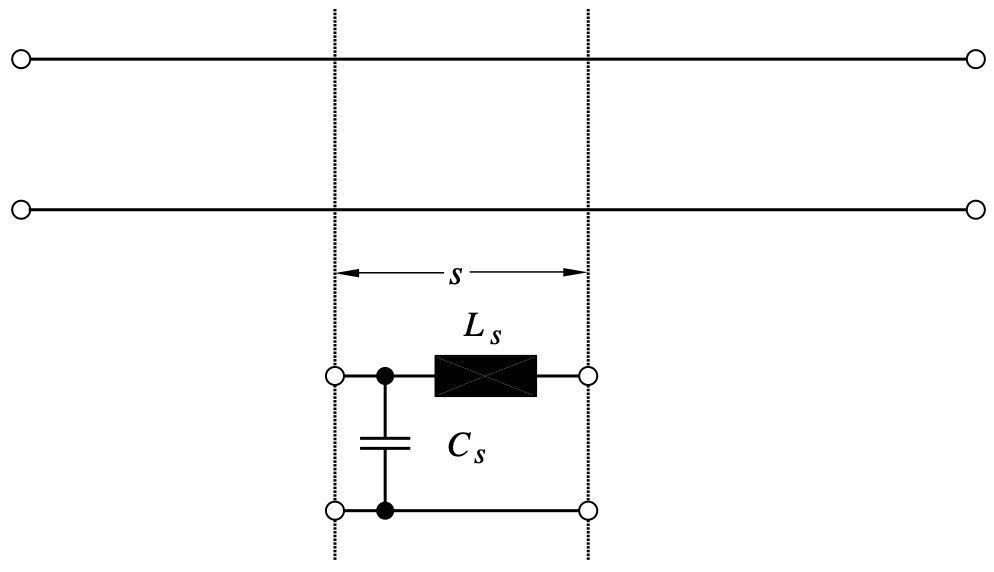
\includegraphics[width=0.5\textwidth]{images/Leitung1.png}
        \caption{Elektrische Leiter mit ihren Anwendungen. Entnommen aus~\cite{LeitungenUndFilter}.}
        \label{Leitung1}
    \end{center}
\end{figure}

Der Fluss $\Phi$ des magnetischen Feldes $\textbf{H}$ bewirkt eine Induktivität $L_{s}$
\[ \Phi_{s} = i \cdot L_{s} \], wobei $i$ der Strom ist.
Das elektrische Feld $\textbf{E}$ induziert Ladungen auf der Oberfläche des Leiters und damit eine Kapazität $C_{s}$,
die über die Spannung $u$ wie folgt zusammenhängt,
\[ Q_{s} = C_{s} \cdot u . \]
Die gesamte Leitung stellen wir uns aus diesen Leitungsstücken zusammengesetzt vor wie auf Abbildung~\ref{Leitung2}
dargestellt.
\begin{figure}[!h]
    \begin{center}
        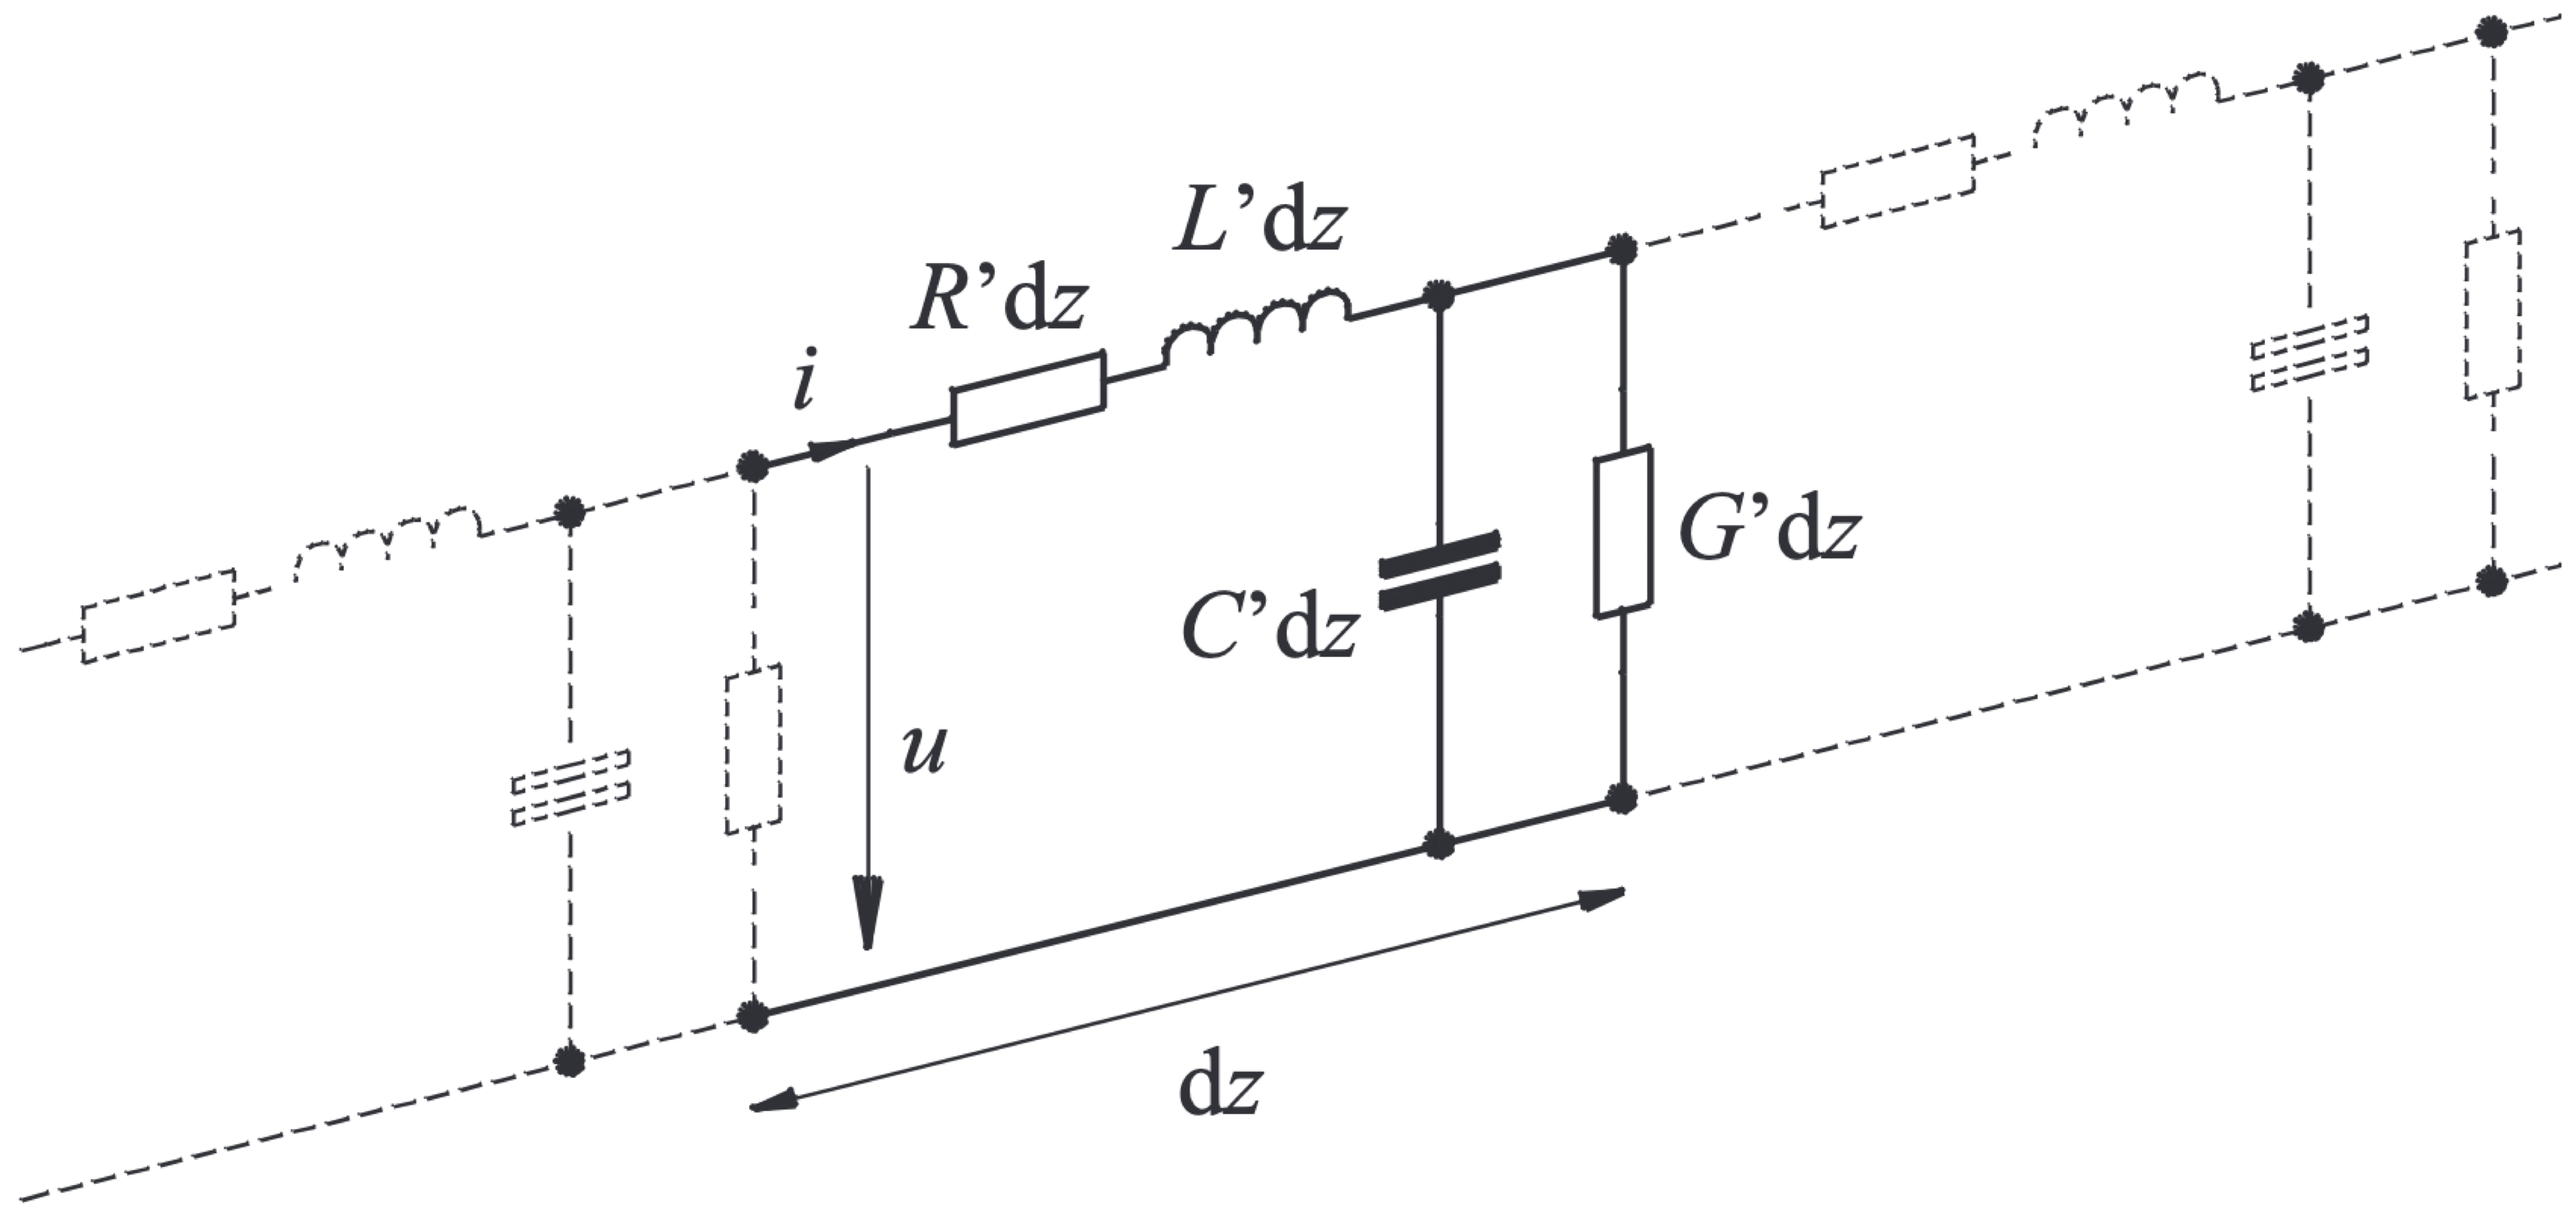
\includegraphics[width=0.5\textwidth]{images/Leitung2.png}
        \caption{Elektrische Leiter mit ihren Anwendungen. Entnommen aus~\cite{LeitungenUndFilter}.}
        \label{Leitung2}
    \end{center}
\end{figure}
Die führt auf die folgenden qualitativen Eigenschaften: Wir eine Spannung am Leitungsanfang angelegt, muss zunächst die
erste Kapazität $Q_{s_{1}}$ aufgeladen werden. Erst dann bildet sich eine Spannung an der Längsinduktivität $L_{s_{1}}$
an. Der aufgebaute Strom wird nun $Q{s_{2}}$ aufladen etc., bis zum Leiterende. Die Ausbreitung des Einschaltvorgangs
findet mit endlicher Geschwindigkeit statt.

Ein elektrischer Strom, der durch einen Leiter fließt, erfährt einen Widerstand $R_{s}$ auf einer Strecke
$\mathrm{d}s$. Wenn wir annehmen, dass das den Leiter umgebende Dielektrikum leitend ist, dann bezeichnen wir dies mit
dem Querleitwert
$G_{s}$ auf der Strecke $\mathrm{d}s$. Die Abbildung~\ref{Leitung3}
\begin{figure}[!h]
    \begin{center}
        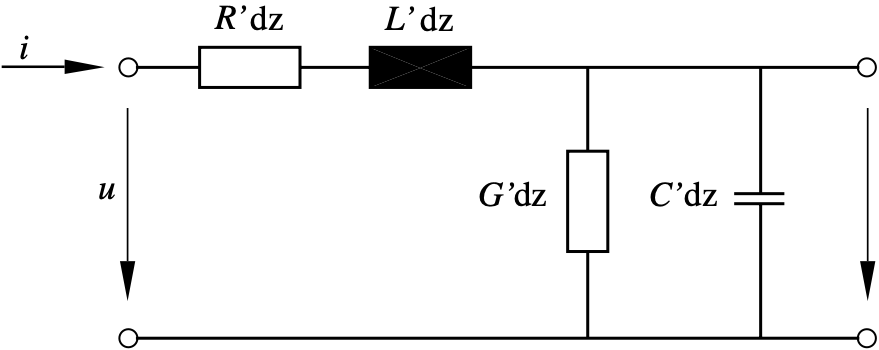
\includegraphics[width=0.5\textwidth]{images/Leitungsstueck.png}
        \caption{Elektrische Leiter mit ihren Anwendungen. Entnommen aus~\cite{LeitungenUndFilter}.}
        \label{Leitung3}
    \end{center}
\end{figure}



\chapter{Die Telegraphenleitungen}
Abbildung~\ref{Leitung4} zeigt nochmals ein infinitesimales Leitungsstück $\mathrm{d}s$ eines verlustbehafteten
Leiters. Am Leitungseingang liegen Strom $i$ und Spannung $u$ an, am Leitungsende $i + \mathrm{d}i$ und $u +
\mathrm{d}u$.
\begin{figure}[!h]
    \begin{center}
        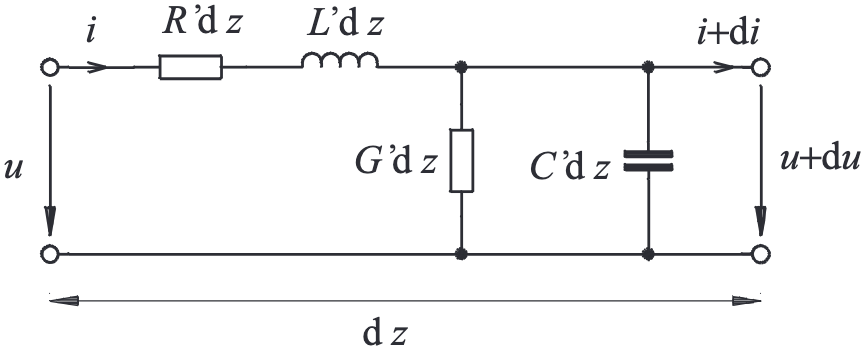
\includegraphics[width=0.5\textwidth]{images/Leitungsstueck2.png}
        \caption{Einschaltbild eines infinitesimalen Leitungsstücks einer verlustbehafteten Leitung. Entnommen
        aus~\cite{LeitungenUndFilter}.}
        \label{Leitung4}
    \end{center}
\end{figure}

Wir definieren auf einem Stück $\mathrm{d}s$

\begin{tabular}{l l}
    den Widerstandsbelag & $R^{\prime} = \frac{R_{s}}{s}$ \\
\addlinespace
    den Induktivitätsbelag & $L^{\prime} = \frac{L_{s}}{s}$ \\
\addlinespace
    den Kapazitätsbelag & $C^{\prime} = \frac{C_{s}}{s}$ \\
\addlinespace
    und den Leitungsbelag & $G^{\prime} = \frac{G_{s}}{s}$. \\
\end{tabular}

Der Widerstand $R^{\prime}$ und die Induktivität $L^{\prime}$ verursachen einen Spannungsabfall von
\[
i \, R^{\prime} \, \mathrm{d}z + \frac{\partial i}{\partial t} \, L^{\prime} \, \mathrm{d} z
\]
entlang von $\mathrm{d}s$. Mit der Kirchhoffschen Maschengleichung {\color{red}REF} folgt für die Spannung
\begin{equation}
u(z, t) = R^{\prime} \, i(z, t) + L^{\prime} \, \frac{\partial i(z, t)}{\partial t} + u(z + \Delta z, t).
\end{equation}
Durch Querleitwert $G_{s}$ und Querkapazität $C_{s}$ fließt der Strom
\[
u \, G^{\prime} \, \mathrm{d}z + \frac{\partial u}{\partial t} \, C^{\prime} \, \mathrm{d} z.
\]
Mit der Kirchhoffschen Knotenregel {\color{red}REF} folgt
\begin{equation}
    i(z, t) = G^{\prime} \, u(z, t) + C^{\prime} \, \frac{\partial u(z + \Delta z, t)}{\partial t} + i(z + \Delta z, t).
\end{equation}
Wir formen nun beide Gleichungen um,
\begin{align}
\frac{u(z + \Delta z, t) - u(z, t)}{\Delta z} &= \frac{R^{\prime}}{\Delta z} \, i(z, t) + \frac{L^{\prime}}{\Delta z}
\,
\frac{\partial i(z, t)}{\partial t} \\
\frac{i(z + \Delta z, t) - i(z, t)}{\Delta z} &= \frac{G^{\prime}}{\Delta z} \, u(z, t) + \frac{C^{\prime}}{\Delta z}
\, \frac{\partial u(z + \Delta z, t)}{\partial t}.
\end{align}
Mit
\[
\lim_{\Delta x \to 0} \frac{u(x+\Delta x, t)-u(x, t)}{\Delta x} = \frac{\partial u(x, t)}{\partial x} \quad \text{und}
\quad \lim_{\Delta x \to 0} \frac{\Delta R}{\Delta x} = R' \quad \text{folgt}
\]
\begin{align}
    \frac{\partial u}{\partial z} &= -\left(R^{\prime} + L^{\prime}\frac{\partial}{\partial t}\right)i \label{eq:Dgl1}
    \\[1ex]
    \frac{\partial i}{\partial z} &= -\left(G^{\prime} + C^{\prime}\frac{\partial}{\partial t}\right)u \label{eq:Dgl2}
\end{align}
Dies ist ein System partieller linearer Differentialgleichungen 1.~Ordnung mit konstanten Koeffizienten. Sie werden
auch Differentialgleichungen der elektrischen Leitung genannt.
Gleichung~\eqref{eq:Dgl1} beschreibt den Spannungsabfall verursacht durch den Leitungswiderstand $R^{\prime}$ und
Induktivität $L^{\prime}$, siehe Abbildung~\ref{Leitung4}.
Die zweite Gleichung~\eqref{eq:Dgl2} beschreibt den Stromfluss zwischen den Leitern, verursacht durch Kapazität
$C^{\prime}$ und Querleitwert $G^{\prime}$.

Oftmals werden diese Gleichungen in die sogenannten Telegraphenleitungen weiter umgeformt. Dazu leiten wir beide
Gleichungen einmal nach $x$ und einmal nach $t$ ab,
\begin{align}
    \frac{\partial^{2} u}{\partial x^2} &= -R^{\prime} \, \frac{\partial i}{\partial x} - L^{\prime} \,
    \frac{\partial^2 i}{\partial t \,
    \partial x} \label{eq:Dgl3} \\[1ex]
    \frac{\partial^{2} i}{\partial x^2} &= -G^{\prime} \, \frac{\partial u}{\partial x} - C^{\prime} \,
    \frac{\partial^2 u}{\partial t \,
    \partial x} \label{eq:Dgl4} \\[1ex]
    \frac{\partial^{2} u}{\partial x \, \partial t} &= -R^{\prime} \, \frac{\partial i}{\partial t} - L^{\prime} \,
    \frac{\partial^2
    i}{\partial t^{2}} \label{eq:Dgl5} \\[1ex]
    \frac{\partial^{2} i}{\partial x \, \partial t} &= -G^{\prime} \, \frac{\partial u}{\partial t} - C^{\prime} \,
    \frac{\partial^2
    u}{\partial t^{2}} \label{eq:Dgl6}
\end{align}
Wir setzen nun \eqref{eq:Dgl2} und \eqref{eq:Dgl6} in \eqref{eq:Dgl3} und \eqref{eq:Dgl1} und \eqref{eq:Dgl5} in
\eqref{eq:Dgl4} ein und erhalten
\begin{align}
    \frac{\partial^{2} u}{\partial x^{2}} &= R^{\prime} G^{\prime} u(x,t) + (R^{\prime} C^{\prime} + L^{\prime}
    G^{\prime}) \frac{\partial u(x, t)}{\partial t} + L^{\prime} C^{\prime} \frac{\partial^{2} u(x,t)}{\partial t^{2}}
    \\[1.5ex]
    \frac{\partial^{2} i}{\partial x^{2}} &= R^{\prime} G^{\prime} i(x,t) + (R^{\prime} C^{\prime} + L^{\prime}
    G^{\prime}) \frac{\partial i(x, t)}{\partial t} + L^{\prime} C^{\prime} \frac{\partial^{2} i(x, t)}{\partial t^{2}}
\end{align}
Im Allgemeinen wird man diese partiellen Differentialgleichungen nur numerisch lösen können. Im Folgenden werden wir
einige Spezialfälle betrachten, die es uns erlauben, das qualitative Verhalten der Signalausbreitung zu beschreiben.


\subsection{Die Gleichungen der verlustlosen Leitung}
Da die Telegraphenleitungen i.A. nur nummerisch gelöst werden können, wollen wir hier eine vereinfachende Annahme
machen: wir nehmen an, dass die Leitung verlustlos ist, d.h. wir setzen $R^{\prime} = G^{\prime} = 0$. Dies erlaubt es
uns, die Gleichungen exakt zu lösen und somit das qualitative Verhalten der Signalausbreitung zu beschreiben. Die
Gleichungen \eqref{eq:Dgl1} und \eqref{eq:Dgl2} vereinfachen sich zu
\begin{align}
    \frac{\partial u}{\partial z} &= - L^{\prime} \, \frac{\partial i}{\partial t} \label{eq:Dgl7} \\[1ex]
    \frac{\partial i}{\partial z} &= - C^{\prime} \, \frac{\partial u}{\partial t} \label{eq:Dgl8} .
\end{align}
Jede dieser Gleichungen hat die Form der Wellengleichung. Sie sind homogene partielle Differentialgleichungen, deren
Lösung aus zwei Partiallösungen \[ u(x, t) = u_{v}(v t - x) + u_{r}(v t + x) \] und \[ i(x, t) = i_{v}(v t - x) +
i_{r}(v t + x) \]. Wir nehmen hier stets $v > 0$ an. In diesem Fall handelt es sich bei $u_{v}$ bzw. $i_{v}$ um
vorwärts laufende Wellen, bei $u_{r}$ und $i_{r}$ um rücklaufende Wellen. Wir betrachten dazu
Abbildung~\ref{VorwaertsWelle}.
\begin{figure}[!h]
    \begin{center}
        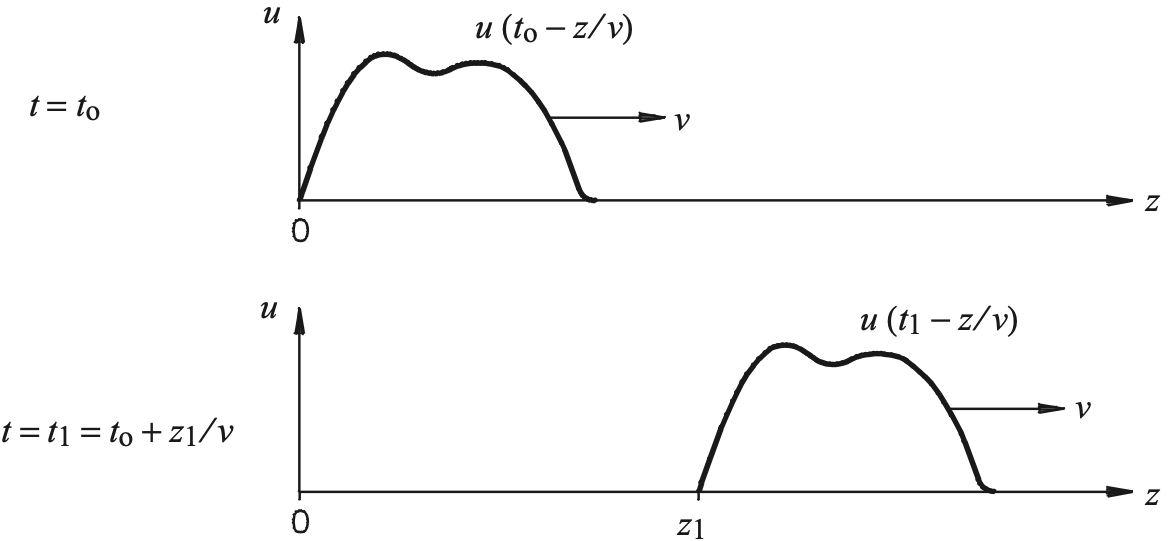
\includegraphics[width=0.75\textwidth]{images/VorwaertsWelle.png}
        \caption{Einschaltbild eines infinitesimalen Leitungsstücks einer verlustbehafteten Leitung. Entnommen
            aus~\cite{LeitungenUndFilter}.}
        \label{VorwaertsWelle}
    \end{center}
\end{figure}
Sei dazu $t_{0} = 0$, $t_{1} > 0$ und $x_{0} > 0$. Dann ist die Welle zum Zeitpunkt $t_{1} > 0$ die Strecke $x = x_{1}
= v t_{1} + x_{0}$ vorangeschritten. Es gilt $u(x_{0}, t_{0}) = u_{v}(-x_{0})$ und
\begin{align*}
    u(x_{1}, t_{1}) &= u_{v}(v t_{1} - x_{1}) \\
                    &= u_{v}(v t_{1} - (v t_{1} + x_{0})) \\
                    &= u_{v}(- x_{0}) \\
                    &= u(x_{0}, t_{0}).
\end{align*}
Wegen $x_{1} > x_{0}$ ist dies also die vorwärts laufende Welle. Analog beschreiben $u_{r}$ bzw. $i_{r}$ jeweils eine
rücklaufende Welle.






\chapter{Telegraphenleitungen}

\section{Verlustloses Model}

\section{Verlustbehaftetes Model}

\section{Abschlüsse}


%\bibliographystyle{plain} % oder ein anderer Stil, z.B. alpha, abbrv, unsrt
%\bibliography{Proseminar} % Name Ihrer .bib-Datei OHNE Endung .bib
\printbibliography

\end{document}
        \includegraphics[width=0.9\linewidth]{../graphics/ElektrischeFeldlinien/document}
        \caption{\color{red}Caption for the second picture}
        \label{Felder2}
    \end{subfigure}
    \caption{\color{red}Overall caption for the figure}
\end{figure}
Analog geht mit einer an den Leitern anliegende Spannung ein elektrischen Feld einher (Abbildung~\ref{Felder2}).
Ändert sich dieses, so hat dies die Ausbildung eines magnetischen Feldes zur Folge, welches mit dem des Stroms
wechselwirkt.


Im Folgenden nehmen wir an, dass der Leiter parallel verläuft, der Abstand $d$ zwischen den Leitern und der Querschnitt
des Leiters viel kleiner ist, als die Wellenlänge $\lambda$ der auftretenden Signale,
\[ d \ll \lambda = \frac{c_{0}}{f \sqrt{\epsilon_{r}}}. \]
In diesem Fall müssen wir nicht die Maxwellschen Gleichungen
lösen -- statt dessen können wir mit der Methode der Ersatzschaltbilder die Signalübertragung direkt mit den
beteiligten Strömen und Spannungen beschreiben, ohne mit den elektrischen und magnetischen Feldern
argumentieren zu müssen.

Es ist $c_{0}$ die Lichtgeschwindigkeit im Vakuum, $f$ die Frequenz des Signals und $\epsilon_{r}$ die relative
Dielektrizitätskonstante bezeichnet. Wir machen hier die vereinfachende Annahme, dass $\epsilon_{r}$ eine (konstante)
Eigenschaft des Mediums ist, in dem sich das Signal ausbreitet. Im Vakuum gilt $\epsilon_{r} = 1$.




Wir betrachten nun ein kleines, infinitesimales Leitungsstück $\mathrm{d}s$,
\begin{figure}[!h]
    \begin{center}
        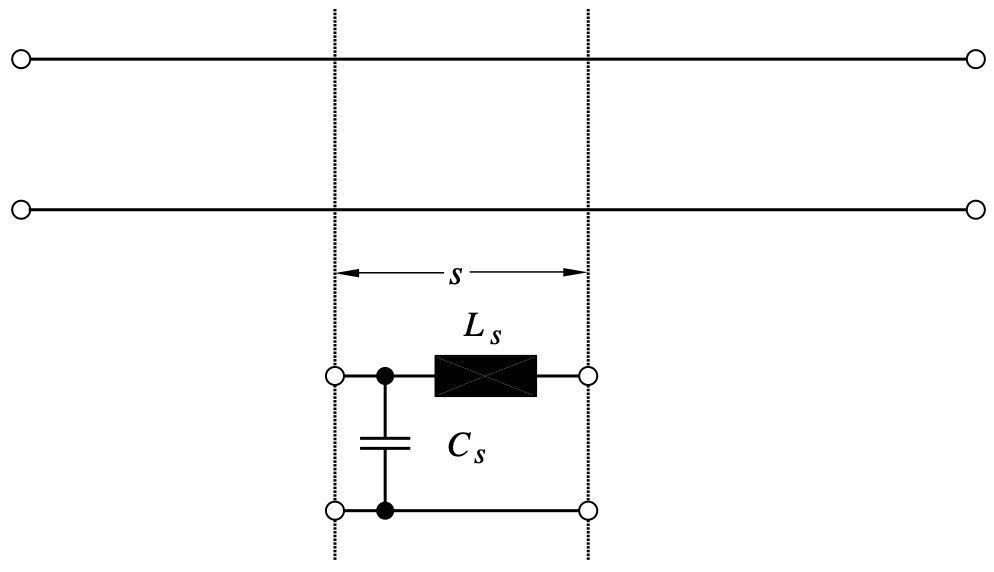
\includegraphics[width=0.5\textwidth]{images/Leitung1.png}
        \caption{Elektrische Leiter mit ihren Anwendungen. Entnommen aus~\cite{LeitungenUndFilter}.}
        \label{Leitung1}
    \end{center}
\end{figure}

Der Fluss $\Phi$ des magnetischen Feldes $\textbf{H}$ bewirkt eine Induktivität $L_{s}$
\[ \Phi_{s} = i \cdot L_{s} \], wobei $i$ der Strom ist.
Das elektrische Feld $\textbf{E}$ induziert Ladungen auf der Oberfläche des Leiters und damit eine Kapazität $C_{s}$,
die über die Spannung $u$ wie folgt zusammenhängt,
\[ Q_{s} = C_{s} \cdot u . \]
Die gesamte Leitung stellen wir uns aus diesen Leitungsstücken zusammengesetzt vor wie auf Abbildung~\ref{Leitung2}
dargestellt.
\begin{figure}[!h]
    \begin{center}
        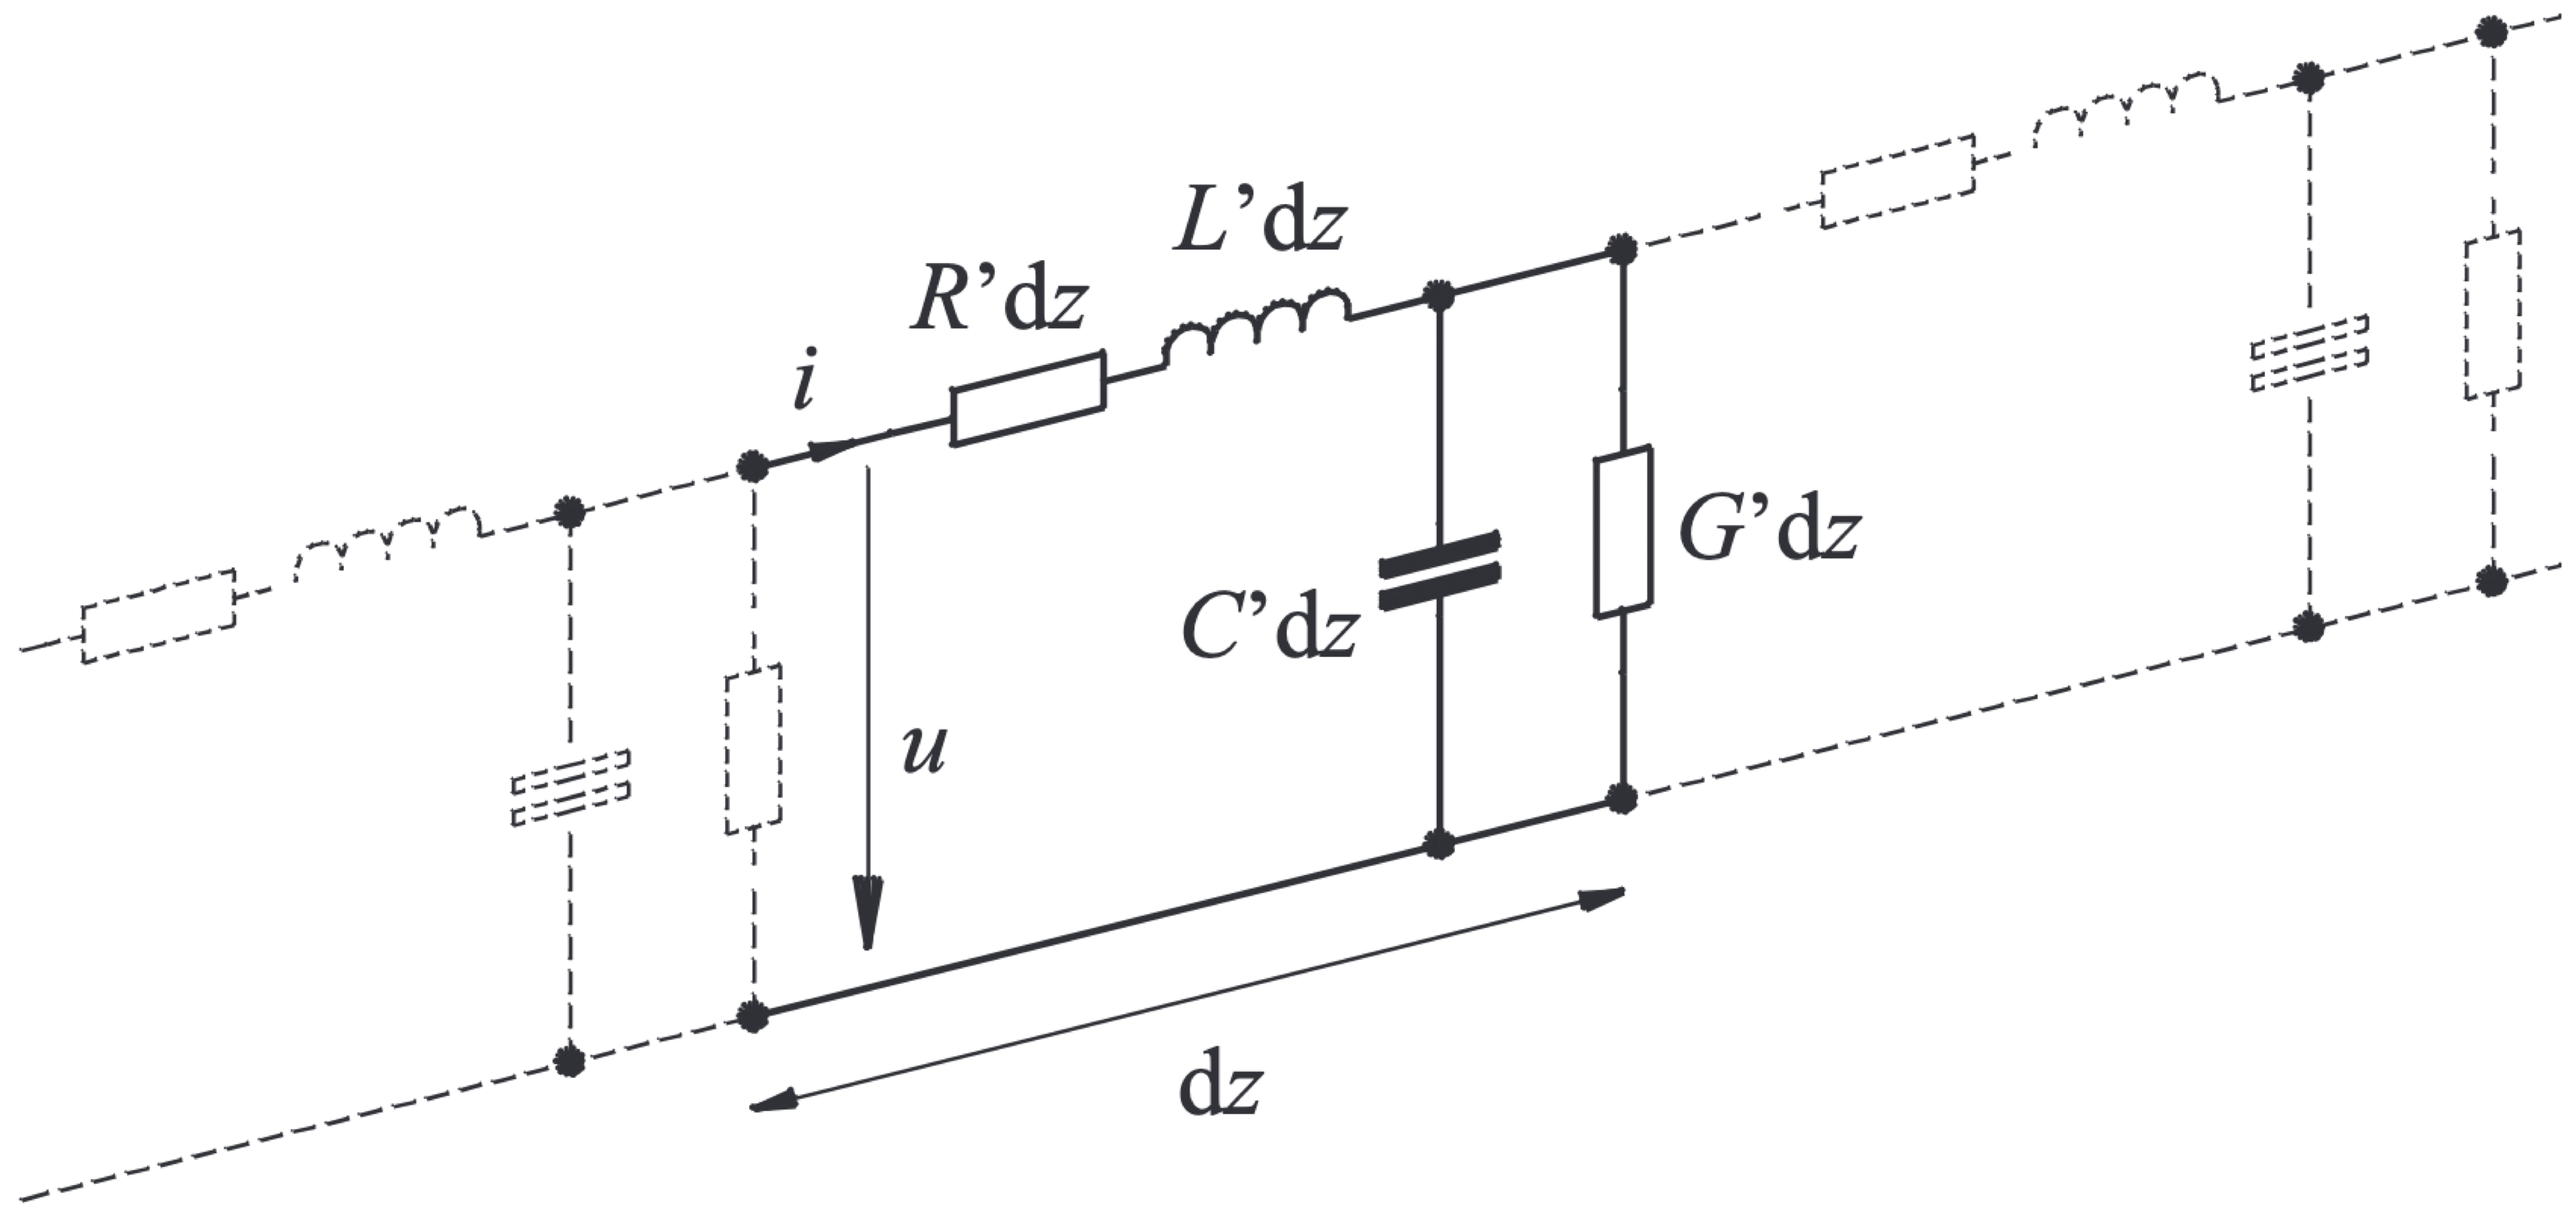
\includegraphics[width=0.5\textwidth]{images/Leitung2.png}
        \caption{Elektrische Leiter mit ihren Anwendungen. Entnommen aus~\cite{LeitungenUndFilter}.}
        \label{Leitung2}
    \end{center}
\end{figure}
Die führt auf die folgenden qualitativen Eigenschaften: Wir eine Spannung am Leitungsanfang angelegt, muss zunächst die
erste Kapazität $Q_{s_{1}}$ aufgeladen werden. Erst dann bildet sich eine Spannung an der Längsinduktivität $L_{s_{1}}$
an. Der aufgebaute Strom wird nun $Q{s_{2}}$ aufladen etc., bis zum Leiterende. Die Ausbreitung des Einschaltvorgangs
findet mit endlicher Geschwindigkeit statt.

Ein elektrischer Strom, der durch einen Leiter fließt, erfährt einen Widerstand $R_{s}$ auf einer Strecke
$\mathrm{d}s$. Wenn wir annehmen, dass das den Leiter umgebende Dielektrikum leitend ist, dann bezeichnen wir dies mit
dem Querleitwert
$G_{s}$ auf der Strecke $\mathrm{d}s$. Die Abbildung~\ref{Leitung3}
\begin{figure}[!h]
    \begin{center}
        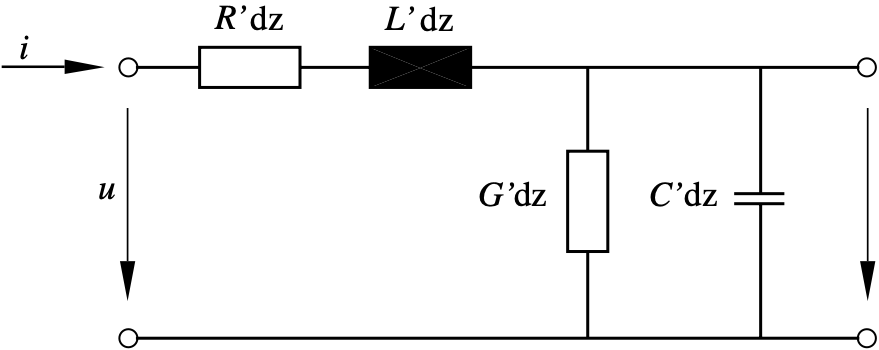
\includegraphics[width=0.5\textwidth]{images/Leitungsstueck.png}
        \caption{Elektrische Leiter mit ihren Anwendungen. Entnommen aus~\cite{LeitungenUndFilter}.}
        \label{Leitung3}
    \end{center}
\end{figure}



\chapter{Die Telegraphenleitungen}
Abbildung~\ref{Leitung4} zeigt nochmals ein infinitesimales Leitungsstück $\mathrm{d}s$ eines verlustbehafteten
Leiters. Am Leitungseingang liegen Strom $i$ und Spannung $u$ an, am Leitungsende $i + \mathrm{d}i$ und $u +
\mathrm{d}u$.
\begin{figure}[!h]
    \begin{center}
        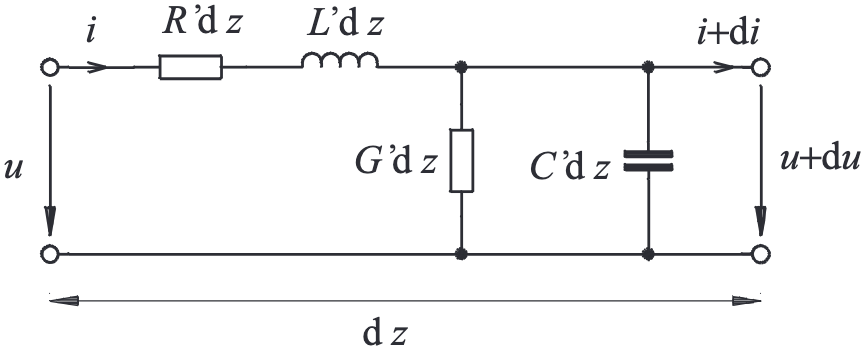
\includegraphics[width=0.5\textwidth]{images/Leitungsstueck2.png}
        \caption{Einschaltbild eines infinitesimalen Leitungsstücks einer verlustbehafteten Leitung. Entnommen
        aus~\cite{LeitungenUndFilter}.}
        \label{Leitung4}
    \end{center}
\end{figure}

Wir definieren auf einem Stück $\mathrm{d}s$

\begin{tabular}{l l}
    den Widerstandsbelag & $R^{\prime} = \frac{R_{s}}{s}$ \\
\addlinespace
    den Induktivitätsbelag & $L^{\prime} = \frac{L_{s}}{s}$ \\
\addlinespace
    den Kapazitätsbelag & $C^{\prime} = \frac{C_{s}}{s}$ \\
\addlinespace
    und den Leitungsbelag & $G^{\prime} = \frac{G_{s}}{s}$. \\
\end{tabular}

Der Widerstand $R^{\prime}$ und die Induktivität $L^{\prime}$ verursachen einen Spannungsabfall von
\[
i \, R^{\prime} \, \mathrm{d}z + \frac{\partial i}{\partial t} \, L^{\prime} \, \mathrm{d} z
\]
entlang von $\mathrm{d}s$. Mit der Kirchhoffschen Maschengleichung {\color{red}REF} folgt für die Spannung
\begin{equation}
u(z, t) = R^{\prime} \, i(z, t) + L^{\prime} \, \frac{\partial i(z, t)}{\partial t} + u(z + \Delta z, t).
\end{equation}
Durch Querleitwert $G_{s}$ und Querkapazität $C_{s}$ fließt der Strom
\[
u \, G^{\prime} \, \mathrm{d}z + \frac{\partial u}{\partial t} \, C^{\prime} \, \mathrm{d} z.
\]
Mit der Kirchhoffschen Knotenregel {\color{red}REF} folgt
\begin{equation}
    i(z, t) = G^{\prime} \, u(z, t) + C^{\prime} \, \frac{\partial u(z + \Delta z, t)}{\partial t} + i(z + \Delta z, t).
\end{equation}
Wir formen nun beide Gleichungen um,
\begin{align}
\frac{u(z + \Delta z, t) - u(z, t)}{\Delta z} &= \frac{R^{\prime}}{\Delta z} \, i(z, t) + \frac{L^{\prime}}{\Delta z}
\,
\frac{\partial i(z, t)}{\partial t} \\
\frac{i(z + \Delta z, t) - i(z, t)}{\Delta z} &= \frac{G^{\prime}}{\Delta z} \, u(z, t) + \frac{C^{\prime}}{\Delta z}
\, \frac{\partial u(z + \Delta z, t)}{\partial t}.
\end{align}
Mit
\[
\lim_{\Delta x \to 0} \frac{u(x+\Delta x, t)-u(x, t)}{\Delta x} = \frac{\partial u(x, t)}{\partial x} \quad \text{und}
\quad \lim_{\Delta x \to 0} \frac{\Delta R}{\Delta x} = R' \quad \text{folgt}
\]
\begin{align}
    \frac{\partial u}{\partial z} &= -\left(R^{\prime} + L^{\prime}\frac{\partial}{\partial t}\right)i \label{eq:Dgl1}
    \\[1ex]
    \frac{\partial i}{\partial z} &= -\left(G^{\prime} + C^{\prime}\frac{\partial}{\partial t}\right)u \label{eq:Dgl2}
\end{align}
Dies ist ein System partieller linearer Differentialgleichungen 1.~Ordnung mit konstanten Koeffizienten. Sie werden
auch Differentialgleichungen der elektrischen Leitung genannt.
Gleichung~\eqref{eq:Dgl1} beschreibt den Spannungsabfall verursacht durch den Leitungswiderstand $R^{\prime}$ und
Induktivität $L^{\prime}$, siehe Abbildung~\ref{Leitung4}.
Die zweite Gleichung~\eqref{eq:Dgl2} beschreibt den Stromfluss zwischen den Leitern, verursacht durch Kapazität
$C^{\prime}$ und Querleitwert $G^{\prime}$.

Oftmals werden diese Gleichungen in die sogenannten Telegraphenleitungen weiter umgeformt. Dazu leiten wir beide
Gleichungen einmal nach $x$ und einmal nach $t$ ab,
\begin{align}
    \frac{\partial^{2} u}{\partial x^2} &= -R^{\prime} \, \frac{\partial i}{\partial x} - L^{\prime} \,
    \frac{\partial^2 i}{\partial t \,
    \partial x} \label{eq:Dgl3} \\[1ex]
    \frac{\partial^{2} i}{\partial x^2} &= -G^{\prime} \, \frac{\partial u}{\partial x} - C^{\prime} \,
    \frac{\partial^2 u}{\partial t \,
    \partial x} \label{eq:Dgl4} \\[1ex]
    \frac{\partial^{2} u}{\partial x \, \partial t} &= -R^{\prime} \, \frac{\partial i}{\partial t} - L^{\prime} \,
    \frac{\partial^2
    i}{\partial t^{2}} \label{eq:Dgl5} \\[1ex]
    \frac{\partial^{2} i}{\partial x \, \partial t} &= -G^{\prime} \, \frac{\partial u}{\partial t} - C^{\prime} \,
    \frac{\partial^2
    u}{\partial t^{2}} \label{eq:Dgl6}
\end{align}
Wir setzen nun \eqref{eq:Dgl2} und \eqref{eq:Dgl6} in \eqref{eq:Dgl3} und \eqref{eq:Dgl1} und \eqref{eq:Dgl5} in
\eqref{eq:Dgl4} ein und erhalten
\begin{align}
    \frac{\partial^{2} u}{\partial x^{2}} &= R^{\prime} G^{\prime} u(x,t) + (R^{\prime} C^{\prime} + L^{\prime}
    G^{\prime}) \frac{\partial u(x, t)}{\partial t} + L^{\prime} C^{\prime} \frac{\partial^{2} u(x,t)}{\partial t^{2}}
    \\[1.5ex]
    \frac{\partial^{2} i}{\partial x^{2}} &= R^{\prime} G^{\prime} i(x,t) + (R^{\prime} C^{\prime} + L^{\prime}
    G^{\prime}) \frac{\partial i(x, t)}{\partial t} + L^{\prime} C^{\prime} \frac{\partial^{2} i(x, t)}{\partial t^{2}}
\end{align}
Im Allgemeinen wird man diese partiellen Differentialgleichungen nur numerisch lösen können. Im Folgenden werden wir
einige Spezialfälle betrachten, die es uns erlauben, das qualitative Verhalten der Signalausbreitung zu beschreiben.


\subsection{Die Gleichungen der verlustlosen Leitung}
Da die Telegraphenleitungen i.A. nur nummerisch gelöst werden können, wollen wir hier eine vereinfachende Annahme
machen: wir nehmen an, dass die Leitung verlustlos ist, d.h. wir setzen $R^{\prime} = G^{\prime} = 0$. Dies erlaubt es
uns, die Gleichungen exakt zu lösen und somit das qualitative Verhalten der Signalausbreitung zu beschreiben. Die
Gleichungen \eqref{eq:Dgl1} und \eqref{eq:Dgl2} vereinfachen sich zu
\begin{align}
    \frac{\partial u}{\partial z} &= - L^{\prime} \, \frac{\partial i}{\partial t} \label{eq:Dgl7} \\[1ex]
    \frac{\partial i}{\partial z} &= - C^{\prime} \, \frac{\partial u}{\partial t} \label{eq:Dgl8} .
\end{align}
Jede dieser Gleichungen hat die Form der Wellengleichung. Sie sind homogene partielle Differentialgleichungen, deren
Lösung aus zwei Partiallösungen \[ u(x, t) = u_{v}(v t - x) + u_{r}(v t + x) \] und \[ i(x, t) = i_{v}(v t - x) +
i_{r}(v t + x) \]. Wir nehmen hier stets $v > 0$ an. In diesem Fall handelt es sich bei $u_{v}$ bzw. $i_{v}$ um
vorwärts laufende Wellen, bei $u_{r}$ und $i_{r}$ um rücklaufende Wellen. Wir betrachten dazu
Abbildung~\ref{VorwaertsWelle}.
\begin{figure}[!h]
    \begin{center}
        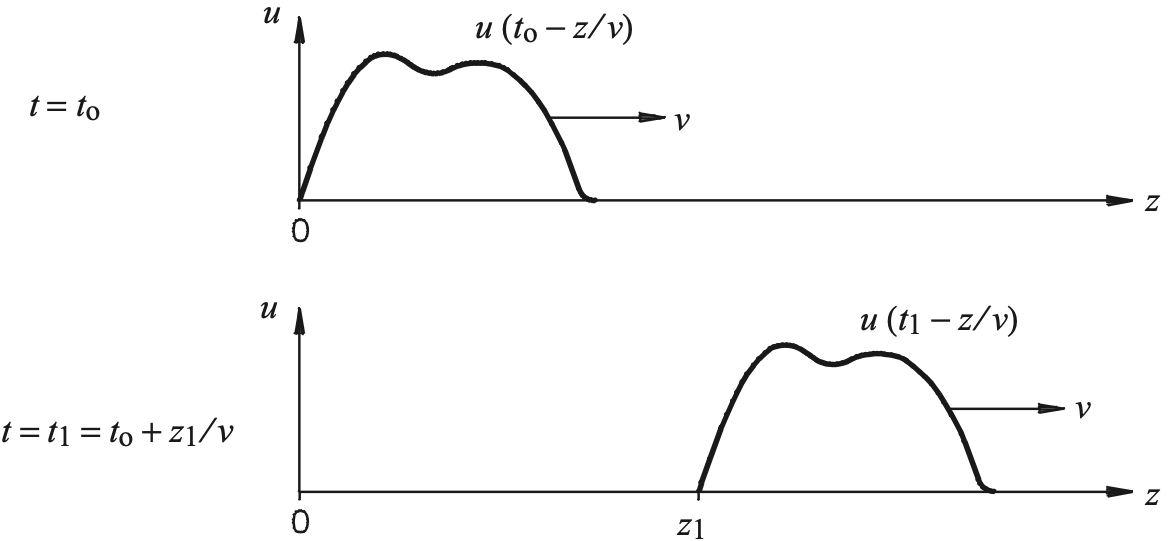
\includegraphics[width=0.75\textwidth]{images/VorwaertsWelle.png}
        \caption{Einschaltbild eines infinitesimalen Leitungsstücks einer verlustbehafteten Leitung. Entnommen
            aus~\cite{LeitungenUndFilter}.}
        \label{VorwaertsWelle}
    \end{center}
\end{figure}
Sei dazu $t_{0} = 0$, $t_{1} > 0$ und $x_{0} > 0$. Dann ist die Welle zum Zeitpunkt $t_{1} > 0$ die Strecke $x = x_{1}
= v t_{1} + x_{0}$ vorangeschritten. Es gilt $u(x_{0}, t_{0}) = u_{v}(-x_{0})$ und
\begin{align*}
    u(x_{1}, t_{1}) &= u_{v}(v t_{1} - x_{1}) \\
                    &= u_{v}(v t_{1} - (v t_{1} + x_{0})) \\
                    &= u_{v}(- x_{0}) \\
                    &= u(x_{0}, t_{0}).
\end{align*}
Wegen $x_{1} > x_{0}$ ist dies also die vorwärts laufende Welle. Analog beschreiben $u_{r}$ bzw. $i_{r}$ jeweils eine
rücklaufende Welle.






\chapter{Telegraphenleitungen}

\section{Verlustloses Model}

\section{Verlustbehaftetes Model}

\section{Abschlüsse}


%\bibliographystyle{plain} % oder ein anderer Stil, z.B. alpha, abbrv, unsrt
%\bibliography{Proseminar} % Name Ihrer .bib-Datei OHNE Endung .bib
\printbibliography

\end{document}
        \includegraphics[width=0.9\linewidth]{../graphics/ElektrischeFeldlinien/document}
        \caption{\color{red}Caption for the second picture}
        \label{Felder2}
    \end{subfigure}
    \caption{\color{red}Overall caption for the figure}
\end{figure}
Analog geht mit einer an den Leitern anliegende Spannung ein elektrischen Feld einher (Abbildung~\ref{Felder2}).
Ändert sich dieses, so hat dies die Ausbildung eines magnetischen Feldes zur Folge, welches mit dem des Stroms
wechselwirkt.


Im Folgenden nehmen wir an, dass der Leiter parallel verläuft, der Abstand $d$ zwischen den Leitern und der Querschnitt
des Leiters viel kleiner ist, als die Wellenlänge $\lambda$ der auftretenden Signale,
\[ d \ll \lambda = \frac{c_{0}}{f \sqrt{\epsilon_{r}}}. \]
In diesem Fall müssen wir nicht die Maxwellschen Gleichungen
lösen -- statt dessen können wir mit der Methode der Ersatzschaltbilder die Signalübertragung direkt mit den
beteiligten Strömen und Spannungen beschreiben, ohne mit den elektrischen und magnetischen Feldern
argumentieren zu müssen.

Es ist $c_{0}$ die Lichtgeschwindigkeit im Vakuum, $f$ die Frequenz des Signals und $\epsilon_{r}$ die relative
Dielektrizitätskonstante bezeichnet. Wir machen hier die vereinfachende Annahme, dass $\epsilon_{r}$ eine (konstante)
Eigenschaft des Mediums ist, in dem sich das Signal ausbreitet. Im Vakuum gilt $\epsilon_{r} = 1$.




Wir betrachten nun ein kleines, infinitesimales Leitungsstück $\mathrm{d}s$,
\begin{figure}[!h]
    \begin{center}
        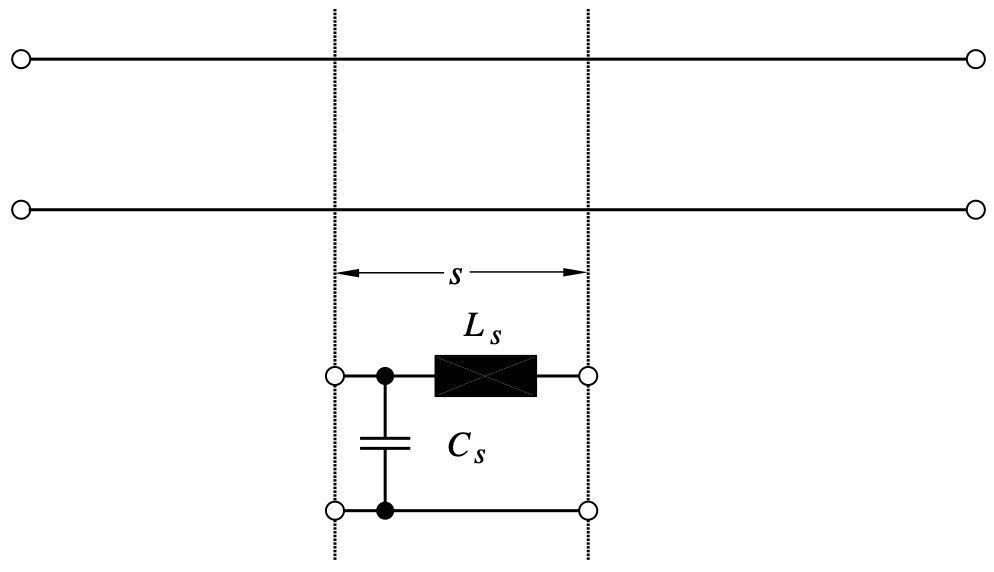
\includegraphics[width=0.5\textwidth]{images/Leitung1.png}
        \caption{Elektrische Leiter mit ihren Anwendungen. Entnommen aus~\cite{LeitungenUndFilter}.}
        \label{Leitung1}
    \end{center}
\end{figure}

Der Fluss $\Phi$ des magnetischen Feldes $\textbf{H}$ bewirkt eine Induktivität $L_{s}$
\[ \Phi_{s} = i \cdot L_{s} \], wobei $i$ der Strom ist.
Das elektrische Feld $\textbf{E}$ induziert Ladungen auf der Oberfläche des Leiters und damit eine Kapazität $C_{s}$,
die über die Spannung $u$ wie folgt zusammenhängt,
\[ Q_{s} = C_{s} \cdot u . \]
Die gesamte Leitung stellen wir uns aus diesen Leitungsstücken zusammengesetzt vor wie auf Abbildung~\ref{Leitung2}
dargestellt.
\begin{figure}[!h]
    \begin{center}
        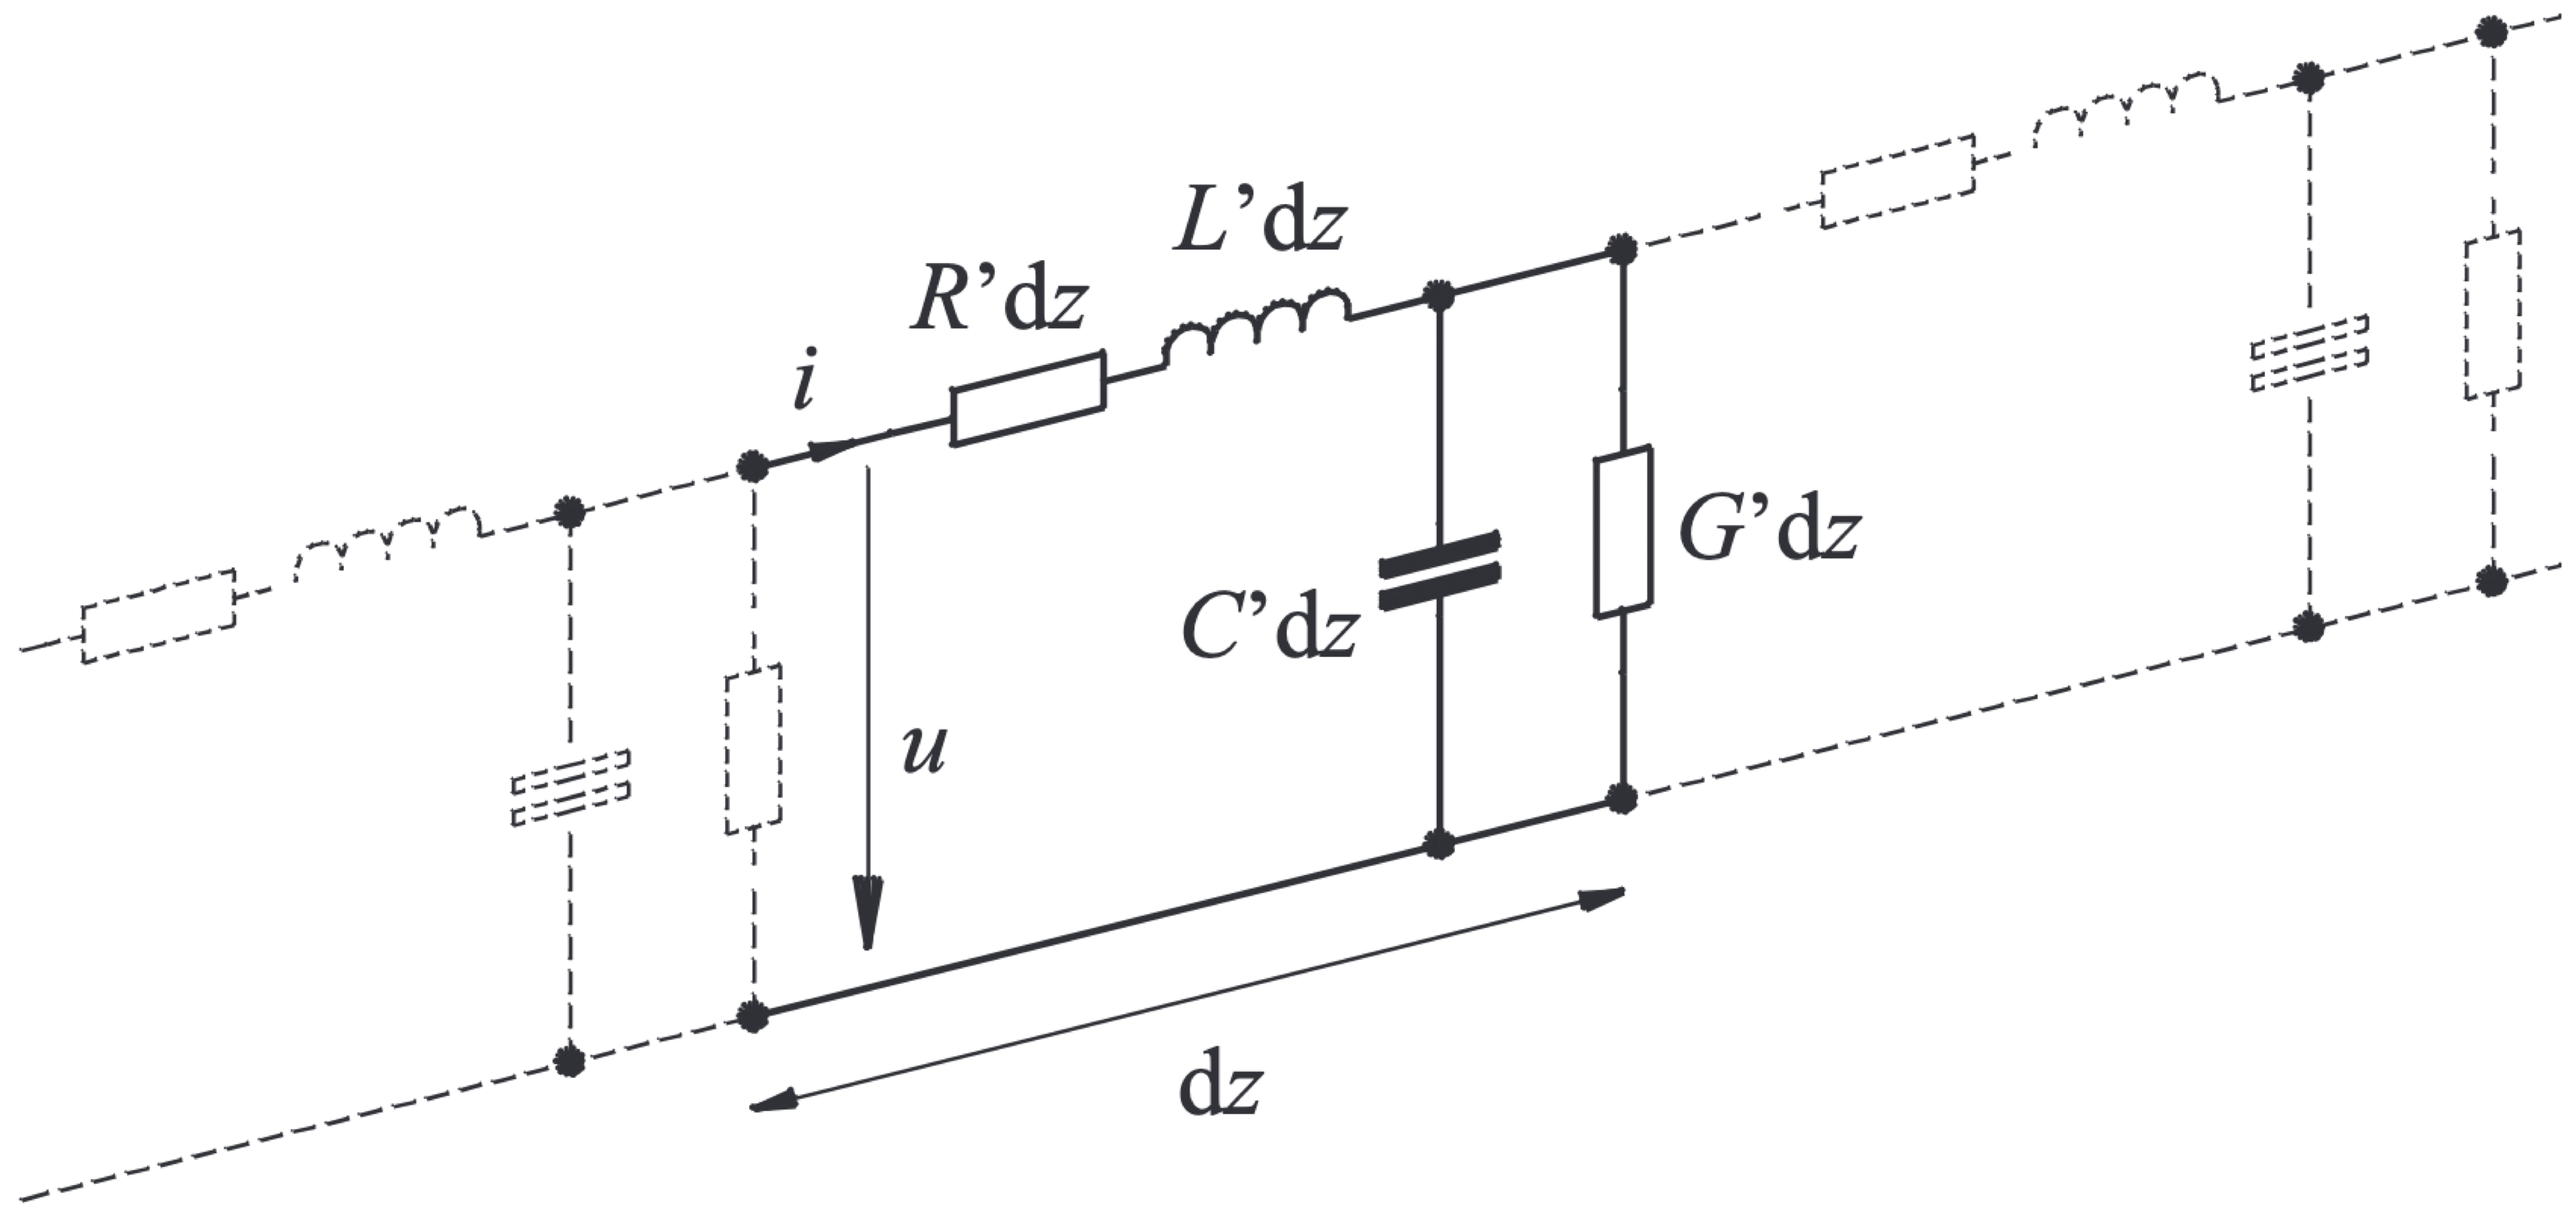
\includegraphics[width=0.5\textwidth]{images/Leitung2.png}
        \caption{Elektrische Leiter mit ihren Anwendungen. Entnommen aus~\cite{LeitungenUndFilter}.}
        \label{Leitung2}
    \end{center}
\end{figure}
Die führt auf die folgenden qualitativen Eigenschaften: Wir eine Spannung am Leitungsanfang angelegt, muss zunächst die
erste Kapazität $Q_{s_{1}}$ aufgeladen werden. Erst dann bildet sich eine Spannung an der Längsinduktivität $L_{s_{1}}$
an. Der aufgebaute Strom wird nun $Q{s_{2}}$ aufladen etc., bis zum Leiterende. Die Ausbreitung des Einschaltvorgangs
findet mit endlicher Geschwindigkeit statt.

Ein elektrischer Strom, der durch einen Leiter fließt, erfährt einen Widerstand $R_{s}$ auf einer Strecke
$\mathrm{d}s$. Wenn wir annehmen, dass das den Leiter umgebende Dielektrikum leitend ist, dann bezeichnen wir dies mit
dem Querleitwert
$G_{s}$ auf der Strecke $\mathrm{d}s$. Die Abbildung~\ref{Leitung3}
\begin{figure}[!h]
    \begin{center}
        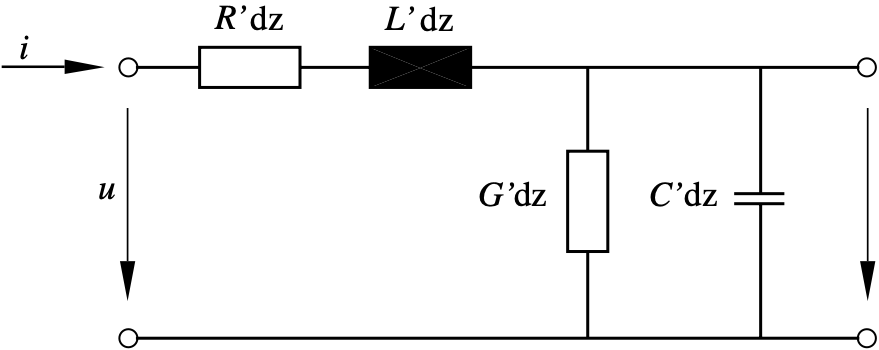
\includegraphics[width=0.5\textwidth]{images/Leitungsstueck.png}
        \caption{Elektrische Leiter mit ihren Anwendungen. Entnommen aus~\cite{LeitungenUndFilter}.}
        \label{Leitung3}
    \end{center}
\end{figure}



\chapter{Die Telegraphenleitungen}
Abbildung~\ref{Leitung4} zeigt nochmals ein infinitesimales Leitungsstück $\mathrm{d}s$ eines verlustbehafteten
Leiters. Am Leitungseingang liegen Strom $i$ und Spannung $u$ an, am Leitungsende $i + \mathrm{d}i$ und $u +
\mathrm{d}u$.
\begin{figure}[!h]
    \begin{center}
        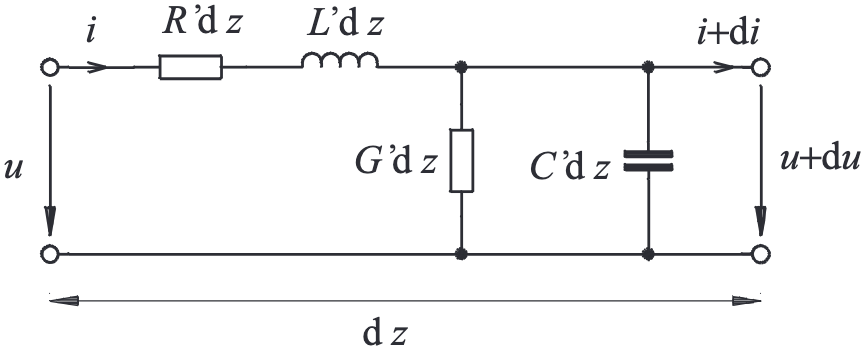
\includegraphics[width=0.5\textwidth]{images/Leitungsstueck2.png}
        \caption{Einschaltbild eines infinitesimalen Leitungsstücks einer verlustbehafteten Leitung. Entnommen
        aus~\cite{LeitungenUndFilter}.}
        \label{Leitung4}
    \end{center}
\end{figure}

Wir definieren auf einem Stück $\mathrm{d}s$

\begin{tabular}{l l}
    den Widerstandsbelag & $R^{\prime} = \frac{R_{s}}{s}$ \\
\addlinespace
    den Induktivitätsbelag & $L^{\prime} = \frac{L_{s}}{s}$ \\
\addlinespace
    den Kapazitätsbelag & $C^{\prime} = \frac{C_{s}}{s}$ \\
\addlinespace
    und den Leitungsbelag & $G^{\prime} = \frac{G_{s}}{s}$. \\
\end{tabular}

Der Widerstand $R^{\prime}$ und die Induktivität $L^{\prime}$ verursachen einen Spannungsabfall von
\[
i \, R^{\prime} \, \mathrm{d}z + \frac{\partial i}{\partial t} \, L^{\prime} \, \mathrm{d} z
\]
entlang von $\mathrm{d}s$. Mit der Kirchhoffschen Maschengleichung {\color{red}REF} folgt für die Spannung
\begin{equation}
u(z, t) = R^{\prime} \, i(z, t) + L^{\prime} \, \frac{\partial i(z, t)}{\partial t} + u(z + \Delta z, t).
\end{equation}
Durch Querleitwert $G_{s}$ und Querkapazität $C_{s}$ fließt der Strom
\[
u \, G^{\prime} \, \mathrm{d}z + \frac{\partial u}{\partial t} \, C^{\prime} \, \mathrm{d} z.
\]
Mit der Kirchhoffschen Knotenregel {\color{red}REF} folgt
\begin{equation}
    i(z, t) = G^{\prime} \, u(z, t) + C^{\prime} \, \frac{\partial u(z + \Delta z, t)}{\partial t} + i(z + \Delta z, t).
\end{equation}
Wir formen nun beide Gleichungen um,
\begin{align}
\frac{u(z + \Delta z, t) - u(z, t)}{\Delta z} &= \frac{R^{\prime}}{\Delta z} \, i(z, t) + \frac{L^{\prime}}{\Delta z}
\,
\frac{\partial i(z, t)}{\partial t} \\
\frac{i(z + \Delta z, t) - i(z, t)}{\Delta z} &= \frac{G^{\prime}}{\Delta z} \, u(z, t) + \frac{C^{\prime}}{\Delta z}
\, \frac{\partial u(z + \Delta z, t)}{\partial t}.
\end{align}
Mit
\[
\lim_{\Delta x \to 0} \frac{u(x+\Delta x, t)-u(x, t)}{\Delta x} = \frac{\partial u(x, t)}{\partial x} \quad \text{und}
\quad \lim_{\Delta x \to 0} \frac{\Delta R}{\Delta x} = R' \quad \text{folgt}
\]
\begin{align}
    \frac{\partial u}{\partial z} &= -\left(R^{\prime} + L^{\prime}\frac{\partial}{\partial t}\right)i \label{eq:Dgl1}
    \\[1ex]
    \frac{\partial i}{\partial z} &= -\left(G^{\prime} + C^{\prime}\frac{\partial}{\partial t}\right)u \label{eq:Dgl2}
\end{align}
Dies ist ein System partieller linearer Differentialgleichungen 1.~Ordnung mit konstanten Koeffizienten. Sie werden
auch Differentialgleichungen der elektrischen Leitung genannt.
Gleichung~\eqref{eq:Dgl1} beschreibt den Spannungsabfall verursacht durch den Leitungswiderstand $R^{\prime}$ und
Induktivität $L^{\prime}$, siehe Abbildung~\ref{Leitung4}.
Die zweite Gleichung~\eqref{eq:Dgl2} beschreibt den Stromfluss zwischen den Leitern, verursacht durch Kapazität
$C^{\prime}$ und Querleitwert $G^{\prime}$.

Oftmals werden diese Gleichungen in die sogenannten Telegraphenleitungen weiter umgeformt. Dazu leiten wir beide
Gleichungen einmal nach $x$ und einmal nach $t$ ab,
\begin{align}
    \frac{\partial^{2} u}{\partial x^2} &= -R^{\prime} \, \frac{\partial i}{\partial x} - L^{\prime} \,
    \frac{\partial^2 i}{\partial t \,
    \partial x} \label{eq:Dgl3} \\[1ex]
    \frac{\partial^{2} i}{\partial x^2} &= -G^{\prime} \, \frac{\partial u}{\partial x} - C^{\prime} \,
    \frac{\partial^2 u}{\partial t \,
    \partial x} \label{eq:Dgl4} \\[1ex]
    \frac{\partial^{2} u}{\partial x \, \partial t} &= -R^{\prime} \, \frac{\partial i}{\partial t} - L^{\prime} \,
    \frac{\partial^2
    i}{\partial t^{2}} \label{eq:Dgl5} \\[1ex]
    \frac{\partial^{2} i}{\partial x \, \partial t} &= -G^{\prime} \, \frac{\partial u}{\partial t} - C^{\prime} \,
    \frac{\partial^2
    u}{\partial t^{2}} \label{eq:Dgl6}
\end{align}
Wir setzen nun \eqref{eq:Dgl2} und \eqref{eq:Dgl6} in \eqref{eq:Dgl3} und \eqref{eq:Dgl1} und \eqref{eq:Dgl5} in
\eqref{eq:Dgl4} ein und erhalten
\begin{align}
    \frac{\partial^{2} u}{\partial x^{2}} &= R^{\prime} G^{\prime} u(x,t) + (R^{\prime} C^{\prime} + L^{\prime}
    G^{\prime}) \frac{\partial u(x, t)}{\partial t} + L^{\prime} C^{\prime} \frac{\partial^{2} u(x,t)}{\partial t^{2}}
    \\[1.5ex]
    \frac{\partial^{2} i}{\partial x^{2}} &= R^{\prime} G^{\prime} i(x,t) + (R^{\prime} C^{\prime} + L^{\prime}
    G^{\prime}) \frac{\partial i(x, t)}{\partial t} + L^{\prime} C^{\prime} \frac{\partial^{2} i(x, t)}{\partial t^{2}}
\end{align}
Im Allgemeinen wird man diese partiellen Differentialgleichungen nur numerisch lösen können. Im Folgenden werden wir
einige Spezialfälle betrachten, die es uns erlauben, das qualitative Verhalten der Signalausbreitung zu beschreiben.


\subsection{Die Gleichungen der verlustlosen Leitung}
Da die Telegraphenleitungen i.A. nur nummerisch gelöst werden können, wollen wir hier eine vereinfachende Annahme
machen: wir nehmen an, dass die Leitung verlustlos ist, d.h. wir setzen $R^{\prime} = G^{\prime} = 0$. Dies erlaubt es
uns, die Gleichungen exakt zu lösen und somit das qualitative Verhalten der Signalausbreitung zu beschreiben. Die
Gleichungen \eqref{eq:Dgl1} und \eqref{eq:Dgl2} vereinfachen sich zu
\begin{align}
    \frac{\partial u}{\partial z} &= - L^{\prime} \, \frac{\partial i}{\partial t} \label{eq:Dgl7} \\[1ex]
    \frac{\partial i}{\partial z} &= - C^{\prime} \, \frac{\partial u}{\partial t} \label{eq:Dgl8} .
\end{align}
Jede dieser Gleichungen hat die Form der Wellengleichung. Sie sind homogene partielle Differentialgleichungen, deren
Lösung aus zwei Partiallösungen \[ u(x, t) = u_{v}(v t - x) + u_{r}(v t + x) \] und \[ i(x, t) = i_{v}(v t - x) +
i_{r}(v t + x) \]. Wir nehmen hier stets $v > 0$ an. In diesem Fall handelt es sich bei $u_{v}$ bzw. $i_{v}$ um
vorwärts laufende Wellen, bei $u_{r}$ und $i_{r}$ um rücklaufende Wellen. Wir betrachten dazu
Abbildung~\ref{VorwaertsWelle}.
\begin{figure}[!h]
    \begin{center}
        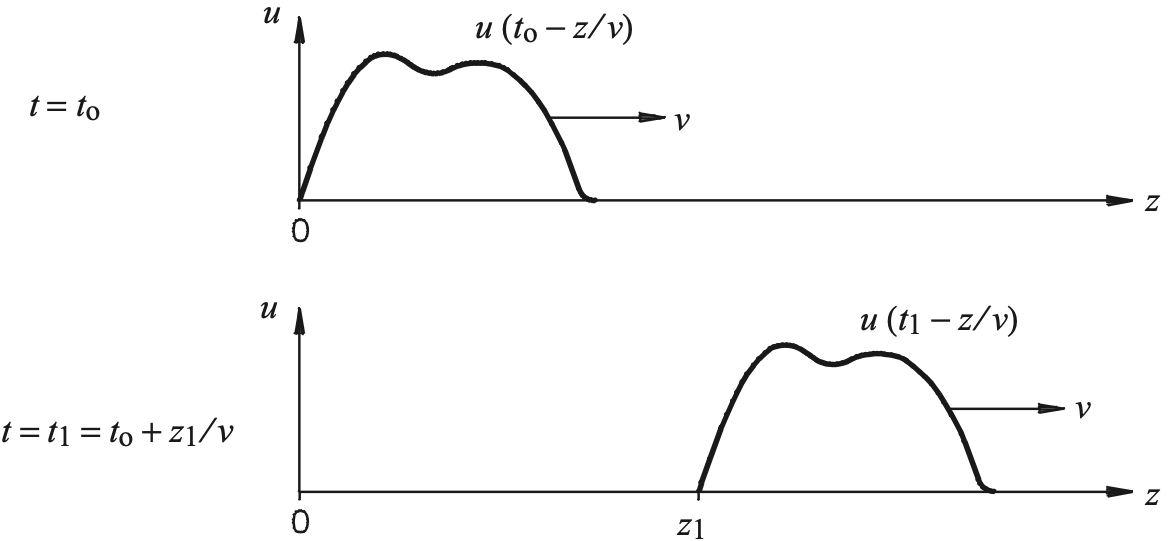
\includegraphics[width=0.75\textwidth]{images/VorwaertsWelle.png}
        \caption{Einschaltbild eines infinitesimalen Leitungsstücks einer verlustbehafteten Leitung. Entnommen
            aus~\cite{LeitungenUndFilter}.}
        \label{VorwaertsWelle}
    \end{center}
\end{figure}
Sei dazu $t_{0} = 0$, $t_{1} > 0$ und $x_{0} > 0$. Dann ist die Welle zum Zeitpunkt $t_{1} > 0$ die Strecke $x = x_{1}
= v t_{1} + x_{0}$ vorangeschritten. Es gilt $u(x_{0}, t_{0}) = u_{v}(-x_{0})$ und
\begin{align*}
    u(x_{1}, t_{1}) &= u_{v}(v t_{1} - x_{1}) \\
                    &= u_{v}(v t_{1} - (v t_{1} + x_{0})) \\
                    &= u_{v}(- x_{0}) \\
                    &= u(x_{0}, t_{0}).
\end{align*}
Wegen $x_{1} > x_{0}$ ist dies also die vorwärts laufende Welle. Analog beschreiben $u_{r}$ bzw. $i_{r}$ jeweils eine
rücklaufende Welle.






\chapter{Telegraphenleitungen}

\section{Verlustloses Model}

\section{Verlustbehaftetes Model}

\section{Abschlüsse}


%\bibliographystyle{plain} % oder ein anderer Stil, z.B. alpha, abbrv, unsrt
%\bibliography{Proseminar} % Name Ihrer .bib-Datei OHNE Endung .bib
\printbibliography

\end{document}
        \caption{\color{red}Caption for the second picture}
        \label{Felder2}
    \end{subfigure}
    \caption{\color{red}Overall caption for the figure}
\end{figure}
Analog geht mit einer an den Leitern anliegende Spannung ein elektrischen Feld einher (Abbildung~\ref{Felder2}).
Ändert sich dieses, so hat dies die Ausbildung eines magnetischen Feldes zur Folge, welches mit dem des Stroms
wechselwirkt.


Im Folgenden nehmen wir an, dass der Leiter parallel verläuft, der Abstand $d$ zwischen den Leitern und der Querschnitt
des Leiters viel kleiner ist, als die Wellenlänge $\lambda$ der auftretenden Signale,
\[ d \ll \lambda = \frac{c_{0}}{f \sqrt{\epsilon_{r}}}. \]
In diesem Fall müssen wir nicht die Maxwellschen Gleichungen
lösen -- statt dessen können wir mit der Methode der Ersatzschaltbilder die Signalübertragung direkt mit den
beteiligten Strömen und Spannungen beschreiben, ohne mit den elektrischen und magnetischen Feldern
argumentieren zu müssen.

Es ist $c_{0}$ die Lichtgeschwindigkeit im Vakuum, $f$ die Frequenz des Signals und $\epsilon_{r}$ die relative
Dielektrizitätskonstante bezeichnet. Wir machen hier die vereinfachende Annahme, dass $\epsilon_{r}$ eine (konstante)
Eigenschaft des Mediums ist, in dem sich das Signal ausbreitet. Im Vakuum gilt $\epsilon_{r} = 1$.


Wir betrachten nun ein kleines, infinitesimales Leitungsstück $\mathrm{d}x$,
\begin{figure}[!h]
    \begin{center}
        \documentclass{standalone}

\usepackage{tikz}
\usepackage[europeanresistors]{circuitikz}
\usetikzlibrary{arrows.meta}
\usetikzlibrary{calc}

\begin{document}

\begin{circuitikz}[scale=0.7, transform shape]
% top wire
\draw[{Circle[open]}-{Circle[open]}] (0,7) -- (8,7);

%bottom wire
\draw[{Circle[open]}-{Circle[open]}] (0,5) -- (8,5);

%left verical line
\draw[dashed] (2,-1) -- (2,8);

%right verical line
\draw[dashed] (6,-1) -- (6,8);

\draw[Stealth-Stealth] (2, 4.25) -- (6, 4.25) node[pos=0.5, circle, fill=white] {d$x$};

% resistor
\draw[{Circle[open, fill=white]}-] ($(2,3) - (2pt,0)$) -- (3,3);
\draw[-{Circle[open, fill=white]}] (5,3) -- ($(6,3) + (2pt,0)$);
% Resistor (no arrow)
\draw (3,3) to[R, l=$R_{x}$, fill=black] (5,3);


% capacitor
\draw[{Circle[open, fill=white]}-{Circle[open, fill=white]}] ($(2,0) - (2pt,0)$) -- ($(6,0) + (2pt,0)$);
\draw[{Circle[open, fill=black]}-] ($(3,3) + (0, 2pt)$) -- (3,2);
\draw[-{Circle[open, fill=black]}] (3,1) -- ($(3,0) - (0, 2pt)$);
\draw (3,2) to[C, l=$C_{x}$] (3,1);

\end{circuitikz}

\end{document}

        \caption{Elektrische Leiter mit ihren Anwendungen. Entnommen aus~\cite{LeitungenUndFilter}.}
        \label{Leitung1}
    \end{center}
\end{figure}

Der Fluss $\Phi$ des magnetischen Feldes $\textbf{H}$ bewirkt eine Induktivität $L_{x}$
\[ \Phi_{x} = i \cdot L_{x} \], wobei $i$ der Strom ist.
Das elektrische Feld $\textbf{E}$ induziert Ladungen auf der Oberfläche des Leiters und damit eine Kapazität $C_{x}$,
die über die Spannung $u$ wie folgt zusammenhängt,
\[ Q_{x} = C_{x} \cdot u . \]
Die gesamte Leitung stellen wir uns aus diesen Leitungsstücken zusammengesetzt vor wie auf Abbildung~\ref{Leitung2}
dargestellt.
\begin{figure}[!h]
    \begin{center}
        \documentclass{standalone}

\usepackage{tikz}
\usepackage[europeanresistors]{circuitikz}
\usetikzlibrary{decorations.markings}
\usetikzlibrary{arrows.meta}
\usetikzlibrary{calc}
\usetikzlibrary{3d}

\begin{document}

\begin{circuitikz}[x={(15:10mm)}, y={(90:10mm)}, scale=0.5]

\tikzset{
charge/.style={fill=orange!10, draw=orange, circle, radius=0.4},
fieldline/.style={postaction={decorate}, decoration={markings}},
arrow/.style={decoration={mark=at position #1 with {\arrow{Stealth}}}},
reversearrow/.style={decoration={mark=at position #1 with {\arrowreversed{Stealth}}}}
}

\newcommand{\diagram}[1]{

\def\componentWidth{10}

% Index of the active component
\def\activeIndex{2}

\ifnum#1=\activeIndex
    \tikzset{line style/.style={solid, black}}
\tikzset{resistor label/.style={l=$R_{z}$}}
\else
\tikzset{line style/.style={densely dashed, black!30}}
\tikzset{resistor label/.style={}}
\fi

\coordinate (A1) at (#1 * \componentWidth + 1, 3);
\coordinate (A2) at (#1 * \componentWidth + 3, 3);
\coordinate (B1) at (#1 * \componentWidth + 1, 0);
\coordinate (B2) at (#1 * \componentWidth + 3, 0);
\coordinate (C1) at (#1 * \componentWidth + 5, 3);
\coordinate (C2) at (#1 * \componentWidth + 8, 3);
\coordinate (D2) at (#1 * \componentWidth + 8, 0);
\coordinate (E1) at (#1 * \componentWidth + 10, 3);
\coordinate (E2) at (#1 * \componentWidth + 10, 0);
\coordinate (E3) at (#1 * \componentWidth + 11, 3);
\coordinate (E4) at (#1 * \componentWidth + 11, 0);
\coordinate (F1) at ($(B1) - (0, 2ex)$);
\coordinate (F2) at ($(E2) - (0, 2ex)$);

\ifnum#1=\activeIndex
    \draw[fieldline, arrow=0.5, line style] (A1) -- (A2) node[pos=0.5, above] {$i$} node[pos=0.2] (A3) {};
\else
    \draw[line style] (A1) -- (A2) node[pos=0.2] (A3) {};
\fi

\draw[line style] (B1) -- (B2) node[pos=0.2] (B3) {};
\draw[-{Circle[open, fill=white]}, line style] (B2) -- ($(D2) + (2pt, 0)$);

\ifnum#1=\activeIndex
    \draw[-Stealth, shorten <= 1ex, shorten >= 1ex, line style] (A3) -- (B3) node[pos=0.5, right] {$u$};
\fi

% resistor
\ifnum#1=\activeIndex
    \draw[line style] (A2) to[R, l=$\Delta R$, fill=black] (C1);
\else
    \draw[line style] (A2) to[R] (C1);
\fi

% inductor
\ctikzset{inductor=american}
    \ifnum#1=\activeIndex
\draw[line style] (C1) to[L, l=$\Delta L$] (C2);
\else
    \draw[line style] (C1) to[L] (C2);
\fi

% capacitor
\ifnum#1=\activeIndex
    \draw[line style] (C2) to[C, l=$\Delta C$] (D2);
\else
    \draw[line style] (C2) to[C] (D2);
\fi

\draw[{Circle[open, fill=white]}-{Circle[open, fill=white]}, line style]  ($(C2) - (2pt, 0)$) --  ($(E1) + (2pt, 0)$);
\draw[-{Circle[open, fill=white]}, line style] (D2) --  ($(E2) + (2pt, 0)$);

% G
\ifnum#1=\activeIndex
    \draw[line style] (E1) to[R, l=$\Delta G$] (E2);
\else
    \draw[line style] (E1) to[R] (E2);
\fi

\draw[line style] (E1) -- (E3);
\draw[line style] (E2) -- (E4);

\ifnum#1=\activeIndex
    \draw[Stealth-Stealth] (F1) -- (F2) node[pos=0.5, circle, fill=white, below] {$\Delta z$};
\fi
}

\begin{scope}[canvas is yx plane at z=0, xscale=-1, rotate=90, transform shape]

    \foreach \i in {1, 2, 3} {
        \diagram{\i}
    }

\end{scope}

\end{circuitikz}

\end{document}

        \caption{Elektrische Leiter mit ihren Anwendungen. Entnommen aus~\cite{LeitungenUndFilter}.}
        \label{Leitung2}
    \end{center}
\end{figure}
Die führt auf die folgenden qualitativen Eigenschaften: Wir eine Spannung am Leitungsanfang angelegt, muss zunächst die
erste Kapazität $Q_{s_{1}}$ aufgeladen werden. Erst dann bildet sich eine Spannung an der Längsinduktivität $L_{s_{1}}$
an. Der aufgebaute Strom wird nun $Q{s_{2}}$ aufladen etc., bis zum Leiterende. Die Ausbreitung des Einschaltvorgangs
findet mit endlicher Geschwindigkeit statt.

Ein elektrischer Strom, der durch einen Leiter fließt, erfährt einen Widerstand $R_{s}$ auf einer Strecke
$\mathrm{d}s$. Wenn wir annehmen, dass das den Leiter umgebende Dielektrikum leitend ist, dann bezeichnen wir dies mit
dem Querleitwert
$G_{s}$ auf der Strecke $\mathrm{d}s$. Die Abbildung~\ref{Leitung3}
\begin{figure}[!h]
    \begin{center}
        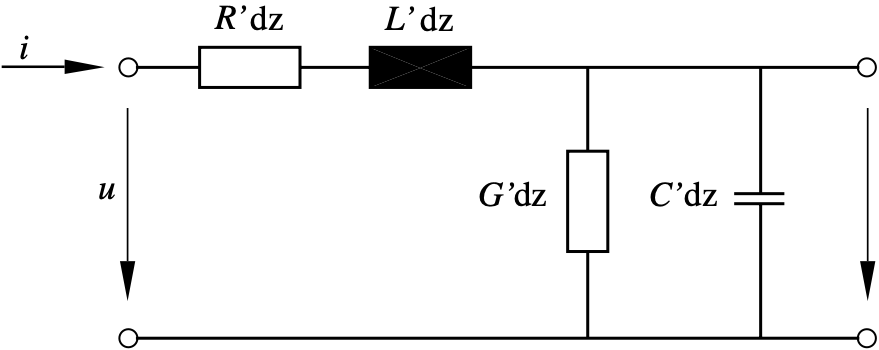
\includegraphics[width=0.5\textwidth]{images/Leitungsstueck.png}
        \caption{Elektrische Leiter mit ihren Anwendungen. Entnommen aus~\cite{LeitungenUndFilter}.}
        \label{Leitung3}
    \end{center}
\end{figure}



\chapter{Die Telegraphenleitungen}
Abbildung~\ref{Leitung4} zeigt nochmals ein infinitesimales Leitungsstück $\mathrm{d}s$ eines verlustbehafteten
Leiters. Am Leitungseingang liegen Strom $i$ und Spannung $u$ an, am Leitungsende $i + \mathrm{d}i$ und $u +
\mathrm{d}u$.
\begin{figure}[!h]
    \begin{center}
        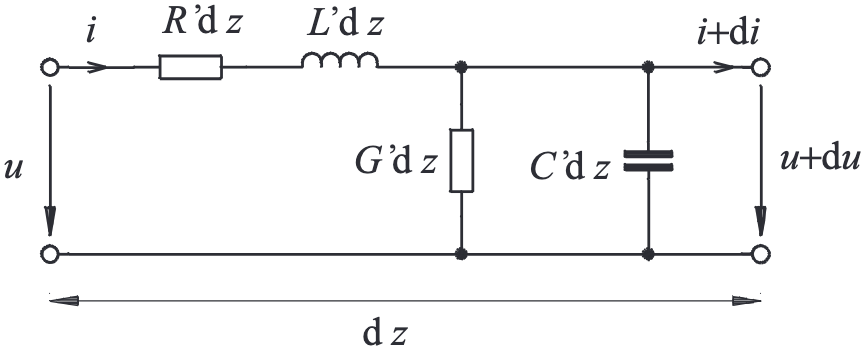
\includegraphics[width=0.5\textwidth]{images/Leitungsstueck2.png}
        \caption{Einschaltbild eines infinitesimalen Leitungsstücks einer verlustbehafteten Leitung. Entnommen
        aus~\cite{LeitungenUndFilter}.}
        \label{Leitung4}
    \end{center}
\end{figure}

Wir definieren auf einem Stück $\mathrm{d}s$

\begin{tabular}{l l}
    den Widerstandsbelag & $R^{\prime} = \frac{R_{s}}{s}$ \\
\addlinespace
    den Induktivitätsbelag & $L^{\prime} = \frac{L_{s}}{s}$ \\
\addlinespace
    den Kapazitätsbelag & $C^{\prime} = \frac{C_{s}}{s}$ \\
\addlinespace
    und den Leitungsbelag & $G^{\prime} = \frac{G_{s}}{s}$. \\
\end{tabular}

Der Widerstand $R^{\prime}$ und die Induktivität $L^{\prime}$ verursachen einen Spannungsabfall von
\[
i \, R^{\prime} \, \mathrm{d}z + \frac{\partial i}{\partial t} \, L^{\prime} \, \mathrm{d} z
\]
entlang von $\mathrm{d}s$. Mit der Kirchhoffschen Maschengleichung {\color{red}REF} folgt für die Spannung
\begin{equation}
u(z, t) = R^{\prime} \, i(z, t) + L^{\prime} \, \frac{\partial i(z, t)}{\partial t} + u(z + \Delta z, t).
\end{equation}
Durch Querleitwert $G_{s}$ und Querkapazität $C_{s}$ fließt der Strom
\[
u \, G^{\prime} \, \mathrm{d}z + \frac{\partial u}{\partial t} \, C^{\prime} \, \mathrm{d} z.
\]
Mit der Kirchhoffschen Knotenregel {\color{red}REF} folgt
\begin{equation}
    i(z, t) = G^{\prime} \, u(z, t) + C^{\prime} \, \frac{\partial u(z + \Delta z, t)}{\partial t} + i(z + \Delta z, t).
\end{equation}
Wir formen nun beide Gleichungen um,
\begin{align}
\frac{u(z + \Delta z, t) - u(z, t)}{\Delta z} &= \frac{R^{\prime}}{\Delta z} \, i(z, t) + \frac{L^{\prime}}{\Delta z}
\,
\frac{\partial i(z, t)}{\partial t} \\
\frac{i(z + \Delta z, t) - i(z, t)}{\Delta z} &= \frac{G^{\prime}}{\Delta z} \, u(z, t) + \frac{C^{\prime}}{\Delta z}
\, \frac{\partial u(z + \Delta z, t)}{\partial t}.
\end{align}
Mit
\[
\lim_{\Delta x \to 0} \frac{u(x+\Delta x, t)-u(x, t)}{\Delta x} = \frac{\partial u(x, t)}{\partial x} \quad \text{und}
\quad \lim_{\Delta x \to 0} \frac{\Delta R}{\Delta x} = R' \quad \text{folgt}
\]
\begin{align}
    \frac{\partial u}{\partial z} &= -\left(R^{\prime} + L^{\prime}\frac{\partial}{\partial t}\right)i \label{eq:Dgl1}
    \\[1ex]
    \frac{\partial i}{\partial z} &= -\left(G^{\prime} + C^{\prime}\frac{\partial}{\partial t}\right)u \label{eq:Dgl2}
\end{align}
Dies ist ein System partieller linearer Differentialgleichungen 1.~Ordnung mit konstanten Koeffizienten. Sie werden
auch Differentialgleichungen der elektrischen Leitung genannt.
Gleichung~\eqref{eq:Dgl1} beschreibt den Spannungsabfall verursacht durch den Leitungswiderstand $R^{\prime}$ und
Induktivität $L^{\prime}$, siehe Abbildung~\ref{Leitung4}.
Die zweite Gleichung~\eqref{eq:Dgl2} beschreibt den Stromfluss zwischen den Leitern, verursacht durch Kapazität
$C^{\prime}$ und Querleitwert $G^{\prime}$.

Oftmals werden diese Gleichungen in die sogenannten Telegraphenleitungen weiter umgeformt. Dazu leiten wir beide
Gleichungen einmal nach $x$ und einmal nach $t$ ab,
\begin{align}
    \frac{\partial^{2} u}{\partial x^2} &= -R^{\prime} \, \frac{\partial i}{\partial x} - L^{\prime} \,
    \frac{\partial^2 i}{\partial t \,
    \partial x} \label{eq:Dgl3} \\[1ex]
    \frac{\partial^{2} i}{\partial x^2} &= -G^{\prime} \, \frac{\partial u}{\partial x} - C^{\prime} \,
    \frac{\partial^2 u}{\partial t \,
    \partial x} \label{eq:Dgl4} \\[1ex]
    \frac{\partial^{2} u}{\partial x \, \partial t} &= -R^{\prime} \, \frac{\partial i}{\partial t} - L^{\prime} \,
    \frac{\partial^2
    i}{\partial t^{2}} \label{eq:Dgl5} \\[1ex]
    \frac{\partial^{2} i}{\partial x \, \partial t} &= -G^{\prime} \, \frac{\partial u}{\partial t} - C^{\prime} \,
    \frac{\partial^2
    u}{\partial t^{2}} \label{eq:Dgl6}
\end{align}
Wir setzen nun \eqref{eq:Dgl2} und \eqref{eq:Dgl6} in \eqref{eq:Dgl3} und \eqref{eq:Dgl1} und \eqref{eq:Dgl5} in
\eqref{eq:Dgl4} ein und erhalten
\begin{align}
    \frac{\partial^{2} u}{\partial x^{2}} &= R^{\prime} G^{\prime} u(x,t) + (R^{\prime} C^{\prime} + L^{\prime}
    G^{\prime}) \frac{\partial u(x, t)}{\partial t} + L^{\prime} C^{\prime} \frac{\partial^{2} u(x,t)}{\partial t^{2}}
     \label{eq:Tele1} \\[1.5ex]
    \frac{\partial^{2} i}{\partial x^{2}} &= R^{\prime} G^{\prime} i(x,t) + (R^{\prime} C^{\prime} + L^{\prime}
    G^{\prime}) \frac{\partial i(x, t)}{\partial t} + L^{\prime} C^{\prime} \frac{\partial^{2} i(x, t)}{\partial t^{2}}
\end{align}
Im Allgemeinen wird man diese partiellen Differentialgleichungen nur numerisch lösen können. Im Folgenden werden wir
einige Spezialfälle betrachten, die es uns erlauben, das qualitative Verhalten der Signalausbreitung zu beschreiben.


\section{Die Gleichungen der verlustlosen Leitung}
\label{VerlustlosesModel}
Da die Telegraphenleitungen i.A. nur nummerisch gelöst werden können, wollen wir hier eine vereinfachende Annahme
machen: wir nehmen an, dass die Leitung verlustlos ist, d.h. wir setzen $R^{\prime} = G^{\prime} = 0$. Dies erlaubt es
uns, die Gleichungen exakt zu lösen und somit das qualitative Verhalten der Signalausbreitung zu beschreiben. Die
Gleichungen \eqref{eq:Dgl1} und \eqref{eq:Dgl2} vereinfachen sich zu
\begin{align}
    \frac{\partial u}{\partial z} &= - L^{\prime} \, \frac{\partial i}{\partial t} \label{eq:Dgl7} \\[1ex]
    \frac{\partial i}{\partial z} &= - C^{\prime} \, \frac{\partial u}{\partial t} \label{eq:Dgl8} .
\end{align}
Jede dieser Gleichungen hat die Form der Wellengleichung. Sie sind homogene partielle Differentialgleichungen, deren
Lösung aus zwei Partiallösungen
\begin{align}
u(x, t) &= u_{v}(v t - x) + u_{r}(v t + x) \label{eq:AllgEq1} \\[1ex]
i(x, t) &= i_{v}(v t - x) + i_{r}(v t + x) \label{eq:AllgEq2}.
\end{align}
Wir nehmen hier stets $v > 0$ an. In diesem Fall handelt es sich bei $u_{v}$ bzw. $i_{v}$ um
vorwärts laufende Wellen, bei $u_{r}$ und $i_{r}$ um rücklaufende Wellen. Wir betrachten dazu
Abbildung~\ref{VorwaertsWelle}.
\begin{figure}[!h]
    \begin{center}
%        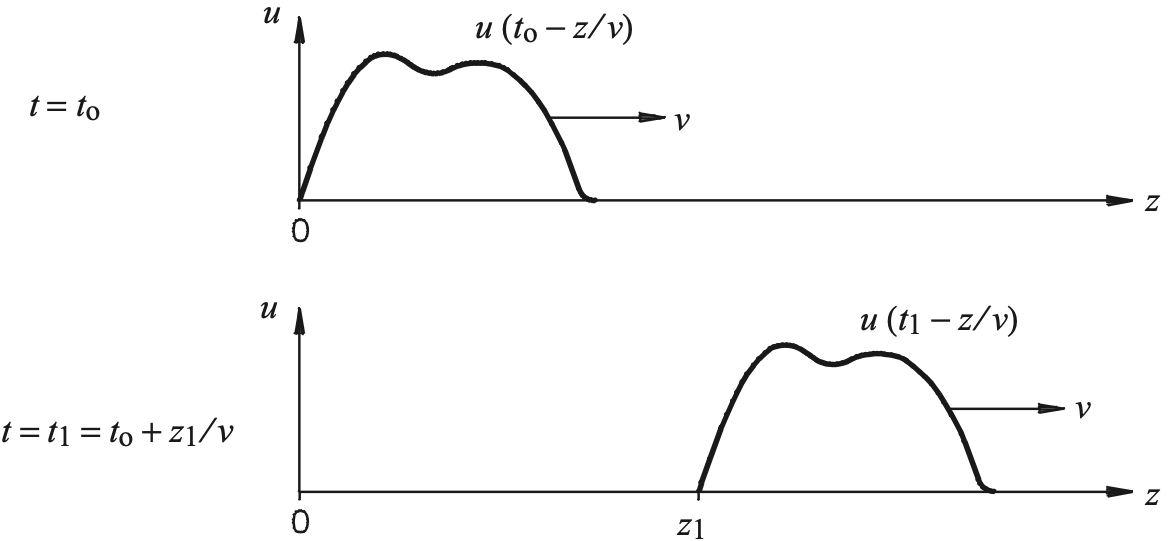
\includegraphics[width=0.75\textwidth]{images/VorwaertsWelle.png}
        \documentclass[tikz]{standalone}
\usepackage{pgfplots}
\pgfplotsset{compat=1.8,
    scale only axis,
    xlabel near ticks,
    ylabel near ticks,
    every axis title shift=3pt}

\usetikzlibrary{arrows.meta}
\usepgfplotslibrary{groupplots}

\begin{document}

\begin{tikzpicture}

\pgfplotsset{xmin=0, xmax=15, ymin=0, ymax=2.5,
    axis lines=left,
    xlabel=$x$,
    ylabel=$\textbf{u}$,
    ylabel style={rotate=-90, at={(current axis.above origin)}, anchor=east},
    xlabel style={at={(axis description cs:1,-0.1)},anchor=north},
    xtick={0},
    yticklabels={},
    % scale y
    y=0.75cm
}

% place outside of plots so negative x shift works
\node[anchor=east] at (-0.1cm, 0.5cm) {$t = t_{0}$};
\node[anchor=east] at (-0.1cm, -2.6cm) {$t = t_{1} = t_{0} + \frac{x_{1}}{v}$};


\begin{groupplot}[group style={group size=1 by 2,
horizontal sep=0pt,
vertical sep=1cm}]

\nextgroupplot[]

\addplot[smooth, samples=100, thick, blue, domain=0:15] coordinates {(0,0) (1,2.3) (2,1.75) (3,2) (4,0) (5,0)}
node[pos=0.6, anchor=south west] {\color{black}$u(v t_{0} - x)$} node[pos=0.75] (A1) {};

\draw[-Stealth] (A1) -- +(1cm,0) node[anchor=west] {$v$};


\nextgroupplot[xtick={0, 7}, xticklabels={0, $x_{1}$},]

\addplot[smooth, samples=100, thick, blue] coordinates {(7,0) (8,2.3) (9,1.75) (10,2) (11,0) (12,0)}
node[pos=0.6, anchor=south west] {\color{black}$u(v t_{1} - x)$} node[pos=0.75] (A1) {};

\draw[-Stealth] (A1) -- +(1cm,0) node[anchor=west] {$v$};

\end{groupplot}

\end{tikzpicture}


\end{document}
        \caption{Einschaltbild eines infinitesimalen Leitungsstücks einer verlustbehafteten Leitung. Entnommen
            aus~\cite{LeitungenUndFilter}.}
        \label{VorwaertsWelle}
    \end{center}
\end{figure}
Sei dazu $t_{0} = 0$, $t_{1} > 0$ und $x_{0} > 0$. Dann ist die Welle zum Zeitpunkt $t_{1} > 0$ die Strecke $x = x_{1}
= v t_{1} + x_{0}$ vorangeschritten. Es gilt $u(x_{0}, t_{0}) = u_{v}(-x_{0})$ und
\begin{align*}
    u(x_{1}, t_{1}) &= u_{v}(v t_{1} - x_{1}) \\
                    &= u_{v}(v t_{1} - (v t_{1} + x_{0})) \\
                    &= u_{v}(- x_{0}) \\
                    &= u(x_{0}, t_{0}).
\end{align*}
Wegen $x_{1} > x_{0}$ ist dies also die vorwärts laufende Welle. Analog beschreiben $u_{r}$ bzw. $i_{r}$ jeweils eine
rücklaufende Welle.


\subsubsection{Wellengeschwindigkeit}

Setzen wir die allgemeine Lösung $u_{v}(v t - x)$ in die Gleichungen \eqref{eq:Dgl7} und \eqref{eq:Dgl8} ein, so
erhalten wir mit
\begin{equation*}
    \frac{\partial u_{v}}{\partial x} = \frac{\partial u_{v}}{\partial w} \frac{\partial w}{\partial x} = -1
    \quad \text{und} \quad
    \frac{\partial u_{v}}{\partial t} = \frac{\partial u_{v}}{\partial w} \frac{\partial w}{\partial t} = v
\end{equation*}
\begin{equation*}
    \frac{\partial^{2} u_{v}}{\partial x^{2}} = -1 \frac{\partial}{\partial x} \left( \frac{\partial u_{v}}{\partial w}
    \right) = -1 \frac{\partial^{2} u_{v}}{\partial w^{2}} \frac{\partial w}{\partial x} = \frac{\partial^{2}
    u_{v}}{\partial w^{2}}
\end{equation*}
und
\begin{equation*}
    \frac{\partial^{2} u_{v}}{\partial t^{2}} = v \frac{\partial}{\partial t} \left( \frac{\partial u_{v}}{\partial w}
    \right) = v \frac{\partial^{2} u_{v}}{\partial w^{2}} \frac{\partial w}{\partial t} =v^{2} \frac{\partial^{2}
        u_{v}}{\partial w^{2}}.
\end{equation*}
Es folgt somit
\begin{equation*}
    \frac{\partial^{2} u_{v}}{\partial x^{2}} = L^{\prime} \, C^{\prime} \, \frac{\partial^{2} u_{v}}{\partial t^{2}}
    \Leftrightarrow
    \frac{\partial^{2} u_{v}}{\partial w^{2}} = L^{\prime} \, C^{\prime} \, v^{2} \frac{\partial^{2} u_{v}}{\partial
    w^{2}}.
\end{equation*}
Nachdem wir die partielle Ableitung herauskürzen, erhalten wir also
\begin{equation}
    v = \frac{1}{\sqrt{L^{\prime} \, C^{\prime}}} \label{eq:WellenGeschw1}.
\end{equation}
überraschend ist nun, dass die Ausbreitungsgeschwindigkeit des Signals im verlustlosen Leiter durch die Parameter
$L^{\prime}$ und $C^{\prime}$ abhängt (und damit vom Isolatormaterial zwischen den Leitern), jedoch nicht vom
Leitermaterial selbst!


\subsubsection{Wellenwiderstand}

Wir kommen nun zu einer weiteren wichtigen Größe, dem Wellenwiderstand.
Setzen wir Gleichungen \eqref{eq:AllgEq1}, \eqref{eq:AllgEq2} und \eqref{eq:WellenGeschw1} in \eqref{eq:Dgl7} und
\eqref{eq:Dgl8} ein, so folgt
\begin{align*}
    \frac{\partial u}{\partial x} &= \frac{\partial u_{v}}{\partial w_{-}} \frac{\partial w_{-}}{\partial x}
    + \frac{\partial u_{r}}{\partial w_{+}} \frac{\partial w_{+}}{\partial x}
    =
    \frac{\partial u_{v}}{\partial w_{-}} \left(- \frac{1}{v} \right) + \frac{\partial u_{r}}{\partial w_{+}}
    \frac{1}{v} \\[1ex]
    \frac{\partial i}{\partial t} &= \frac{\partial i_{v}}{\partial w_{-}} - \frac{\partial i_{r}}{\partial w_{+}}
\end{align*}
und
\begin{align*}
    \frac{\partial i}{\partial x} &= \frac{\partial i_{v}}{\partial w_{-}} \frac{\partial w_{-}}{\partial x}
    + \frac{\partial i_{r}}{\partial w_{+}} \frac{\partial w_{+}}{\partial x}
    =
    \frac{\partial i_{v}}{\partial w_{-}} \left(- \frac{1}{v} \right) - \frac{\partial i_{r}}{\partial w_{+}}
    \frac{1}{v} \\[1ex]
    \frac{\partial u}{\partial t} &= \frac{\partial u_{v}}{\partial w_{-}}
    \underbrace{\frac{\partial w_{-}}{\partial t} }_{=1}
    -
    \frac{\partial u_{r}}{\partial w_{+}} \underbrace{\frac{\partial w_{+}}{\partial t} }_{=1}
\end{align*}
und somit
\begin{alignat*}{3}
    \frac{\partial u}{\partial x} &= \frac{1}{v} \left( \frac{\partial u_{r}}{\partial w_{+}} -
    \frac{\partial u_{v}}{\partial w_{-}} \right) &= - L^{\prime} \left( \frac{\partial i_{v}}{\partial w_{-}} -
    \frac{\partial i_{r}}{\partial w_{+}} \right) &= L^{\prime} \, \frac{\partial i}{\partial t} \\[1ex]
    \frac{\partial i}{\partial x} &= - \frac{1}{v} \left( \frac{\partial i_{r}}{\partial w_{+}} +
    \frac{\partial i_{v}}{\partial w_{-}} \right) &= - C^{\prime} \left( \frac{\partial u_{v}}{\partial w_{+}} +
    \frac{\partial u_{r}}{\partial w_{-}} \right) &= C^{\prime} \, \frac{\partial u}{\partial t}.
\end{alignat*}
Da die Funktionen $u_{v}$ und $u_{r}$ bzw. $i_{v}$ und $i_{r}$ unabhängig sind, folgt
\begin{equation}
    - \frac{1}{v} \, \frac{\text{d} u_{v}}{\text{d} w_{-}} = - L^{\prime} \, \frac{\text{d} i_{v}}{\text{d} w_{-}}.
\end{equation}
Integrieren beider Seiten liefert
\begin{equation}
    u_{v}(w_{-}) = v \, L^{\prime} \, i_{v}(w_{-}) + c_{v} = \sqrt{\frac{L^{\prime}}{C^{\prime}}} \, i_{v}(w_{-}) +
    c_{v},
\end{equation}
und
\begin{equation}
    u_{r}(w_{+}) = v \, L^{\prime} \, i_{r}(w_{+}) + c_{r} = \sqrt{\frac{L^{\prime}}{C^{\prime}}} \, i_{r}(w_{+}) +
    c_{r},
\end{equation}
wobei $c_{v}$ und $c_{r}$ Konstanten sind. Setzen wir $c_{v} = c_{r} = 0$, dann erhalten wir
\begin{equation}
    \frac{u_{v}(x, t)}{i_{v}(x, t)} = \frac{u_{r}(x, t)}{i_{r}(x, t)} = \sqrt{\frac{L^{\prime}}{C^{\prime}}} = Z_{w}.
\end{equation}
Diese Konstante hat die Maßeinheit eines Widerstandes, wir nennen $Z_{w}$ folglich den Wellenwiderstand der Leitung.
Kommen wir nun zur verlustbehafteten Leitung.

\section{Verlustbehaftetes Model}
Wir wollen jetzt für einen weiteren Spezialfall die Telegraphenleitungen lösen. Wir nehmen an, dass das System im
eingeschwungenen Zustand ist. Wir nehmen weiter an, dass die auftretenden Signale aus einer einzigen sin-förmigen
Schwingung fester Frequenz bestehen. I.A. Fall zerlegt man die auftretenden Signale in ihre einzelnen
Frequenzkomponenten und betrachtet diese zunächst getrennt.

Wir stellen Strom und Spannung mittels sogenannter Phasoren $\underline{I}$ und $\underline{U}$ dar, um hervorzuheben,
dass es sich um komplexe Größen handelt:
\begin{align}
    u(x, t) &= \mathrm{Re} \left( \underline{U}(x) \exp(\mathrm{j} \omega t) \right) \label{eq:Spannung} \\
    i(x, t) &= \mathrm{Re} \left( \underline{I}(x) \exp(\mathrm{j} \omega t) \right)
\end{align}
mit $\omega = 2 \pi f$. Es handelt sich hierbei um stationäre sin-förmige Signale, bei denen Ort- und Zeitabhängigkeit
entkoppelt sind.

Das Einsetzen der Phasoren in die Gleichungen \eqref{eq:Dgl1} und \eqref{eq:Dgl2} liefert
\begin{align}
    \frac{\text{d} \underline{U}}{\text{d} x} &= - \left( R^{\prime} + \mathrm{j} \omega L^{\prime} \right)
    \underline{I} \label{eq:ResDgl1} \\[1ex]
    \frac{\text{d} \underline{I}}{\text{d} x} &= - \left( G^{\prime} + \mathrm{j} \omega C^{\prime} \right)
    \underline{U}
\end{align}
Wir eliminieren $\underline{I}$ aus \eqref{eq:ResDgl1} durch nochmaliges Ableiten der Gleichung nach $x$:
\begin{align}
    \frac{\text{d}^{2} \underline{U}}{\text{d} x^{2}} &= \left( R^{\prime} + \mathrm{j} \omega L^{\prime} \right)
    \left( G^{\prime} + \mathrm{j} \omega C^{\prime} \right) \underline{U} \label{eq:ResDgl3}.
\end{align}
Verglichen mit \eqref{eq:Tele1} entfällt in \eqref{eq:ResDgl3} die Zeitabhängigkeit. Damit haben wir eine gewöhnliche
Differentialgleichung 2.~Ordnung mit konstanten Koeffizienten, wir wir sie in Abschnitt~\ref{VerlustlosesModel} bereits
begegnet sind.

Für den Phasor $\underline{I}$ erhalten wir mit ähnlichen Argumenten
\begin{align}
    \frac{\text{d}^{2} \underline{I}}{\text{d} x^{2}} &= \left( R^{\prime} + \mathrm{j} \omega L^{\prime} \right)
    \left( G^{\prime} + \mathrm{j} \omega C^{\prime} \right) \underline{I}.
\end{align}
Dies sind die Wellengleichungen der verlustbehafteten Leitung. Sie werden in der Regel wie folgt geschrieben:
\begin{align}
    \frac{\text{d}^{2} \underline{U}}{\text{d} x^{2}} &= \gamma^{2} \underline{U} \label{eq:VerlustDgl1} \\[1ex]
    \frac{\text{d}^{2} \underline{I}}{\text{d} x^{2}} &= \gamma^{2} \underline{I} \label{eq:VerlustDgl2} \\[1ex]
    \gamma^{2} &= \left( R^{\prime} + \mathrm{j} \omega L^{\prime} \right) \left( G^{\prime} + \mathrm{j} \omega
    C^{\prime} \right).
\end{align}
Man nennt $\gamma$ die Wellenausbreitungsgeschwindigkeit. Verglichen zum verlustlosen Model ist dies eine komplexe
Größe, was dazu führt, dass im verlustbehafteten Fall ein Dämpfungsterm in der Lösung auftritt.

Die allgemeine Lösungen haben die Form
\[ \underline{U}_{1} \exp(- \gamma x) \quad \text{und} \quad \underline{U}_{2} \exp(\gamma x), \] wobei
$\underline{U}_{1}$ und $\underline{U}_{2}$ Integrationskonstanten sind, die durch die Anfangsbedingungen festgelegt
werden.
Es gilt somit für die Spannung
\begin{equation}
    \underline{U}(x) = \underline{U}_{1} \exp(- \gamma x) + \underline{U}_{2} \exp(\gamma x) \label{eq:VerlustU}.
\end{equation}
Die Gleichung für den Strom erhalten wir, wenn wir \eqref{eq:VerlustU} in \eqref{eq:ResDgl1} einsetzen,
\begin{equation}
    \underline{I}(x) = \frac{-1}{R^{\prime} + \mathrm{j} \omega L^{\prime}} \frac{\text{d} \underline{U}}{\text{d} x}
    = \frac{1}{Z}
    \left(
    \vphantom{\sqrt{1}{Z}}
    \underline{U}_{1} \exp(- \gamma x) + \underline{U}_{2} \exp(\gamma x) \right),
\end{equation}
wobei wir
\begin{equation}
    Z_{w} = \sqrt{\frac{G^{\prime} + \mathrm{j} \omega C^{\prime}}{R^{\prime} + \mathrm{j} \omega L^{\prime}}}
    \label{eq:Zw}
\end{equation}
eingeführt haben. $Z$ hat die Dimension eines Widerstandes und wird daher Wellenwiderstand oder Wellenimpedanz
genannt.

\subsubsection{Anfangsbedingungen am Leiteranfang}

Fixieren wir Spannung und Strom am Leiteranfang durch $\underline{U}_{a}$ und $\underline{I}_{a}$, so gilt
\begin{align*}
    \underline{U}(0) &= \underline{U}_{a} = \underline{U}_{1} + \underline{U}_{2} \\[1ex]
    \underline{I}(0) &= \underline{I}_{a} = \frac{1}{Z_{w}}
    \left(
    \vphantom{\sqrt{1}{Z_{w}}}
    \underline{U}_{1} - \underline{U}_{2} \right).
\end{align*}
Für die Integrationskonstanten $\underline{U}_{1}$ und $\underline{U}_{2}$ folgt
\[ \underline{U}_{1} = \frac{\underline{U}_{a} + Z_{w} \underline{I}_{a}}{2} \quad \text{und} \quad \underline{U}_{2} =
\frac{\underline{U}_{a} - Z_{w} \underline{I}_{a}}{2}. \]
Damit lauten die Gleichungen für Spannung und Strom entlang der Leitung
\begin{align}
    \underline{U}(x) &=
    \frac{1}{2} \left( \underline{U}_{a} + Z_{w} \underline{I}_{a} \right) \mathrm{e}^{- \gamma x}
    +
    \frac{1}{2} \left( \underline{U}_{a} - Z_{w} \underline{I}_{a} \right) \mathrm{e}^{\gamma x} \label{eq:UxA} \\[1ex]
    \underline{I}(x) &=
    \frac{1}{2} \left( \frac{\underline{U}_{a}}{Z_{w}} + \underline{I}_{a} \right) \mathrm{e}^{- \gamma x}
    -
    \frac{1}{2} \left( \frac{\underline{U}_{a}}{Z_{w}} - \underline{I}_{a} \right) \mathrm{e}^{\gamma x} \label{eq:IxA}
    .
\end{align}

\subsubsection{Anfangsbedingungen am Leiterende}

Für die spätere Betrachtung ist es hilfreich, die Gleichungen mit Anfangsbedingungen anzugeben, die durch Spannung und
Strom am Leiterende $x=l$, $\underline{U}_{e}$ und $\underline{I}_{e}$, festgelegt sind.
\begin{align*}
    \underline{U}(l) &= \underline{U}_{e} = \underline{U}_{1} \mathrm{e}^{- \gamma l}
    +
    \underline{U}_{2} \mathrm{e}^{ \gamma l} \\[1ex]
    \underline{I}(l) &= \underline{I}_{e} = \frac{1}{Z_{w}}
    \left(
    \underline{U}_{1} \mathrm{e}^{- \gamma l}
    -
    \underline{U}_{2} \mathrm{e}^{ \gamma l}
    \right).
\end{align*}
In diesem Fall gilt für die Integrationskonstanten
\[ \underline{U}_{1} = \frac{\underline{U}_{e} + Z_{w} \underline{I}_{e}}{2} \mathrm{e}^{\gamma x} \quad \text{und}
\quad \underline{U}_{2} = \frac{\underline{U}_{e} - Z_{w} \underline{I}_{e}}{2} \mathrm{e}^{- \gamma x}. \]
Die Gleichungen für Spannung und Strom lauten damit
\begin{align}
    \underline{U}(x) &=
    \frac{1}{2} \left( \underline{U}_{e} + Z_{w} \underline{I}_{e} \right) \mathrm{e}^{\gamma (l - x)}
    +
    \frac{1}{2} \left( \underline{U}_{e} - Z_{w} \underline{I}_{e} \right) \mathrm{e}^{- \gamma (l - x)} \label{eq:UxE}
    \\[1ex]
    \underline{I}(x) &=
    \frac{1}{2} \left( \frac{\underline{U}_{e}}{Z_{w}} + \underline{I}_{e} \right) \mathrm{e}^{\gamma (l - x)}
    -
    \frac{1}{2} \left( \frac{\underline{U}_{e}}{Z_{w}} - \underline{I}_{e} \right) \mathrm{e}^{- \gamma (l - x)}
    \label{eq:IxE} .
\end{align}

Um die Wellenausbreitung entlang des Leiters besser verstehen zu können, spalten wir zunächst die
Wellenausbreitungsgeschwindigkeit $\gamma$ auf in Real- und Imaginärteil:
\[ \gamma = \alpha + \mathrm{j} \beta. \] Wir nennen $\alpha$ die Dämpfungskonstante (oder -belag) und $\beta$ die
Phasenkonstante (oder-belag). Für die Spannung gilt mit \eqref{eq:Spannung}
\begin{equation}
u(x, t) = \mathrm{Re} \left[
\frac{1}{2} \left( \underline{U}_{a} + Z_{w} \underline{I}_{a} \right) \mathrm{e}^{- \alpha x}
\mathrm{e}^{- \mathrm{j} \beta x} \mathrm{e}^{\mathrm{j} \omega t}
+
\frac{1}{2} \left( \underline{U}_{a} - Z_{w} \underline{I}_{a} \right) \mathrm{e}^{\alpha x}
\mathrm{e}^{\mathrm{j} \beta x} \mathrm{e}^{\mathrm{j} \omega t}
\right].
\end{equation}
Wir führen die Abkürzungen
\begin{align*}
\frac{1}{2} \left( \underline{U}_{a} + Z_{w} \underline{I}_{a} \right) &= \hat{U}_{1} \mathrm{e}^{\mathrm{j} \psi_{1}}
\\[1ex]
\frac{1}{2} \left( \underline{U}_{a} - Z_{w} \underline{I}_{a} \right) &= \hat{U}_{2} \mathrm{e}^{\mathrm{j} \psi_{2}}
\end{align*}
ein, mit denen für die Spannung folgt
\begin{equation}
u(x,t) =
\hat{U}_{1} \mathrm{e}^{- \alpha x} \cos \left( \omega t - \beta x + \psi_{1} \right)
+
\hat{U}_{2} \mathrm{e}^{\alpha x} \cos \left( \omega t + \beta x + \psi_{2} \right).
\end{equation}
Die Spannung setzt sich also aus zwei Einzelspannungen zusammen. Der Faktor $\exp(-\alpha x)$ bewirkt ein
exponentiellen Abfall der Teilspannung entlang der positiven $x$-Achse. Für die zweite Teilspannung bewirkt
$\exp(\alpha x)$ einen exponentiellen Abfall in die negative $x$-Richtung der Amplitude.

\subsubsection{Wellenlänge}

Für einen festen Zeitpunkt $t$ oszilliert jede der Teilspannungen entlang der $x$-Richtung, da das Argument des Kosinus
von $x$ abhängt. Für die Periode der Welle gilt gilt \[ \beta z = 2 \pi, \] und somit
\[ x = \lambda = \frac{2 \pi}{\beta}, \] die Wellenlänge der Schwingung. Die ist exemplarisch auf
Abbildung\ref{ExpWelle} gezeigt.
\begin{figure}[!htpb]
    \begin{center}
        \documentclass[tikz]{standalone}
\usepackage{pgfplots}
\pgfplotsset{compat=1.8,
    scale only axis,
    xlabel near ticks,
    ylabel near ticks,
    every axis title shift=3pt}

\usetikzlibrary{arrows.meta}
\usepgfplotslibrary{groupplots}

\begin{document}

\begin{tikzpicture}

\pgfplotsset{xmin=0, xmax=25, ymin=-1.25, ymax=1.25,
    axis x line=center,
    axis y line=left,
    xlabel=$x$,
    ylabel=$\textbf{u}$,
    ylabel style={rotate=-90, at={(current axis.above origin)}, anchor=east},
    xlabel style={at={(axis description cs:1,0.45)},anchor=north},
    xtick={0},
    yticklabels={},
    % scale y
%    y=1cm
}


\begin{groupplot}[group style={group size=1 by 2,
horizontal sep=1cm,
vertical sep=1cm}]

\nextgroupplot[]

%envelope
\addplot[thick, dotted, domain=0:25] {exp(-0.1*x)} node[pos=0.6, left] (A1) {};
\addplot[thick, dotted, domain=0:25] {-exp(-0.1*x)};

\draw (A1) -- +(45:20) node[right, yshift=3pt] {$\mathrm{e}^{- \alpha x}$};

% cos
\addplot[thick, blue, domain=0:25, samples=200] {exp(-0.105*x) * cos(deg(x))} node[pos=0.04, left] (V1) {}
node[pos=0.21] (N1) {} node[pos=0.465] (N2) {};

\draw[thick, orange] (N1) -- +(-90:4cm) node[pos=0.7] (N121) {};
\draw[thick, orange] (N2) -- +(-90:4cm) node[pos=0.7] (N122) {};
\draw[Stealth-Stealth] (N121) -- (N122) node[pos=0.5, fill=white] {$\lambda = \frac{2 \pi}{\beta}$};

\draw[-Stealth] (V1) -- +(0:0.7cm) node[right, inner sep=2pt] {$\textbf{v}$};



\nextgroupplot[]

%envelope
\addplot[thick, dotted, domain=0:25] {exp(-0.1*(25-x))} node[pos=0.6, left] (A1) {};
\addplot[thick, dotted, domain=0:25] {-exp(-0.1*(25-x))};

\draw (A1) -- +(135:20) node[left, inner sep=0] {$\mathrm{e}^{\alpha x}$};

% cos
\addplot[thick, blue, domain=0:25, samples=200] {exp(-0.105*(25-x)) * cos(deg(25-x))} node[pos=0.96, right] (V1) {};

\draw[-Stealth] (V1) -- +(180:0.7cm) node[left, inner sep=2pt] {$-\textbf{v}$};


\end{groupplot}

\end{tikzpicture}


\end{document}
        \caption{Einschaltbild eines infinitesimalen Leitungsstücks einer verlustbehafteten Leitung. Entnommen
            aus~\cite{LeitungenUndFilter}.}
        \label{ExpWelle}
    \end{center}
\end{figure}


\subsubsection{Wellengeschwindigkeit}

Um die Wellengeschwindigkeit zu bestimmen, betrachten wir einen Nulldurchgang einer Teilspannung zum Zeitpunkt
$t=t_{0}$, bei dem das Argument des Kosinus $\frac{\pi}{2}$ sei. Es gilt
\[ x_{0} = \frac{\omega t_{0} + \psi_{1} -\frac{\pi}{2}}{\beta} \]. Nach der Zeit $t_{1} = t_{0} + \Delta t$ sei der
folgende Nulldurchgang erreicht, für den gilt
\[ x_{1} = \frac{\omega t_{1} + \psi_{1} -\frac{\pi}{2}}{\beta} \]. Für die Phasengeschwindigkeit der Welle gilt somit
\[ v = \frac{x_{1} - x_{0}}{t_{1} - t_{0}} = \frac{\omega}{\beta}. \]

Zwar haben wir hier nur Spannungen untersucht, aber aufgrund der Symmetrie der Gleichungen~\eqref{eq:VerlustDgl1} und
\eqref{eq:VerlustDgl2} unterscheidet sich die Gleichung für den Teilstrom nur um den Faktor von der der Teilspannung.
Die Leitungsgleichungen für Strom und Spannung setzen sich aus jeweils zwei Exponentialtermen zusammen, die sich
entlang des Leiters als gedämpfte Wellen in entgegengesetzter Richtung ausbreiten,
\begin{alignat}{2}
\underline{U}_(x) &= \underline{U}_{1} \mathrm{e}^{- \gamma x} + \underline{U}_{2} \mathrm{e}^{\gamma x}
&= \underline{U}_{v} + \underline{U}_{r} \\[1ex]
\underline{I}_(x) &= \underline{I}_{1} \mathrm{e}^{- \gamma x} + \underline{I}_{2} \mathrm{e}^{\gamma x}
&= \underline{I}_{v} + \underline{I}_{r}.
\end{alignat}

Wenn wir das Verhältnis der Teilspannung und Teilstrom bilden, so ergibt sich mit \eqref{eq:UxA} und \eqref{eq:IxA}
\[ \frac{\underline{U}_{1}}{\underline{I}_{1}} = \frac{\underline{U}_{a} + Z_{w}
\underline{I}_{a}}{\frac{\underline{U}_{a}}{Z_{w}} + \underline{I}_{a}} = Z_{w}, \]
der Wellenwiderstand \eqref{eq:Zw}. Für die rücklaufende Welle gilt entsprechend
\[ \frac{\underline{U}_{2}}{-\underline{I}_{2}} = \frac{\underline{U}_{a} - Z_{w}
\underline{I}_{a}}{\frac{\underline{U}_{a}}{Z_{w}} - \underline{I}_{a}} = Z_{w}. \]
Per Konvention sei die positive Stromrichtung die der positiven $x$-Richtung entlang des Leiters.


\section{Reflexionen}

Strom und Spannung entlang des Leiters sind vollständig bestimmt durch die Anfangsbedingungen und $\gamma$, siehe
Gleichungen \eqref{eq:VerlustDgl1} und \eqref{eq:VerlustDgl2}. Es bilden sich zwei Teilwellen aus, die in
entgegengesetzte Richtungen verlaufen. Wir betrachten nun verschiedene Spezialfälle des Leitungsabschlusses um die
Wechselwirkung beider Teilwellen zu verstehen. Wir betrachten explizit das Leiterende, da dort mittels eines
eingefügten Widerstands Diskontinuitäten entstehen, die zu reflektierten Wellen führen.

\subsubsection{Unendlich langer Leiter}

Abbildung~\ref{OhneAbschluss} zeigt eine unendlich lange Leitung. In diesem Fall findet die Signalausbreitung nur in
der positiven $x$-Richtung statt.
\begin{figure}[!htpb]
    \begin{center}
        \documentclass{standalone}

\usepackage{tikz}
\usepackage[europeanresistors]{circuitikz}
\usetikzlibrary{decorations.markings}
\usetikzlibrary{arrows.meta}
\usetikzlibrary{calc}

\begin{document}

\begin{circuitikz}

\tikzset{
    fieldline/.style={postaction={decorate}, decoration={markings}},
    arrow/.style={decoration={mark=at position #1 with {\arrow{Stealth}}}},
    reversearrow/.style={decoration={mark=at position #1 with {\arrowreversed{Stealth}}}},
    line style/.style={solid, black}
    resistor label/.style={l=$R_{x}$}, y=0.75cm}

\coordinate (A1) at (1, 10);
\coordinate (A2) at (3, 10);
\coordinate (A3) at (7, 10);
\coordinate (A4) at (1, 9);
\coordinate (A5) at (1, 7);
\coordinate (A6) at (1, 5);
\coordinate (A7) at (3, 5);
\coordinate (A8) at (7, 5);
\coordinate (A9) at (10, 5);
\coordinate (A10) at (10, 10);

\draw[-{Circle[open, fill=white]}] (A1) -- ($(A2) + (2pt, 0)$) node[above] {$\underline{U}_{a} = Z_{w}
\underline{I}_{a}$};
\draw (A1) -- (A4);

% Lastwiderstand
\draw (A4) to[european resistor, l=$Z_{0}$] (A5);

% voltage source
\draw (A5) to[sinusoidal voltage source, l=$U_{0}$] (A6);

\draw[-{Circle[open, fill=white]}] (A6) -- ($(A7) + (2pt, 0)$);

\draw[-Stealth, shorten >=5pt, shorten <=5pt] (A2) -- (A7) node[pos=0.5, right] {$\underline{U}_{a}$};

\draw[fieldline, arrow=0.5] ($(A2) + (2pt, 0)$) -- (A3);
\draw ($(A7) + (2pt, 0)$) -- (A8);

\draw[dashed] (A3) -- (A10);
\draw[-Stealth, dashed] (A8) -- (A9) node[below] {$x$};

\end{circuitikz}

\end{document}
        \caption{Einschaltbild eines infinitesimalen Leitungsstücks einer verlustbehafteten Leitung. Entnommen
            aus~\cite{LeitungenUndFilter}.}
        \label{OhneAbschluss}
    \end{center}
\end{figure}
Aus den Leitungsgleichungen \eqref{eq:UxE} und \eqref{eq:IxE} folgt, dass die rücklaufende Welle durch den
Dämpfungsterm gegenüber der hinlaufenden Welle vernachlässigt werden kann. Die Leitungsgleichungen vereinfachen sich
mit $\underline{U}_{a} = Z_{w} \underline{I}_{a}$ zu
\[ \underline{U}(x) = \underline{U}_{a} \mathrm{e}^{- \gamma z} \quad \text{und} \quad
 \underline{I}(x) = \frac{\underline{U}_{a}}{Z_{w}} \mathrm{e}^{- \gamma z}. \]

\subsubsection{Anpassung}
Wir betrachten nun den Fall, dass wir die Leitung mit einem Widerstand $Z_{e} = Z_{w}$ schliessen, siehe
Abbildung\ref{AbschlussMitWiderstand}.
\begin{figure}[!htpb]
    \begin{center}
        \documentclass{standalone}

\usepackage{tikz}
\usepackage[europeanresistors]{circuitikz}
\usetikzlibrary{decorations.markings}
\usetikzlibrary{arrows.meta}
\usetikzlibrary{calc}

\begin{document}

\begin{circuitikz}

\tikzset{
    fieldline/.style={postaction={decorate}, decoration={markings}},
    arrow/.style={decoration={mark=at position #1 with {\arrow{Stealth}}}},
    reversearrow/.style={decoration={mark=at position #1 with {\arrowreversed{Stealth}}}},
    line style/.style={solid, black}
    resistor label/.style={l=$R_{x}$}}

\coordinate (A1) at (1, 10);
\coordinate (A2) at (3, 10);
\coordinate (A3) at (7, 10);
\coordinate (A4) at (1, 9);
\coordinate (A5) at (1, 7);
\coordinate (A6) at (1, 5);
\coordinate (A7) at (3, 5);
\coordinate (A8) at (7, 5);
\coordinate (A9) at (9, 10);
\coordinate (A10) at (9, 9);
\coordinate (A11) at (9, 6);
\coordinate (A12) at (9, 5);

\draw (A1) -- ($(A2) + (2pt, 0)$) node[above] {$\underline{U}_{a} = Z_{w} \underline{I}_{a}$};
\draw (A1) -- (A4);

% Lastwiderstand
\draw (A4) to[european resistor, l=$Z_{0}$] (A5);

% voltage source
\draw (A5) to[sinusoidal voltage source, l=$U_{0}$] (A6);

\draw (A6) -- ($(A7) + (2pt, 0)$);

\draw[-Stealth, shorten >=5pt, shorten <=5pt] (A2) -- (A7) node[pos=0.5, right] {$\underline{U}_{a}$};

\draw[{Circle[open, fill=white]}-] ($(A2) + (-2pt, 0)$) -- ($(A2)!0.3!(A3)$);
\draw[dotted] ($(A2)!0.3!(A3)$) -- ($(A2)!0.7!(A3)$);
\draw[-{Circle[open, fill=white]}] ($(A2)!0.7!(A3)$) -- (A3);

\draw[{Circle[open, fill=white]}-] ($(A7) + (-2pt, 0)$) -- ($(A7)!0.3!(A8)$);
\draw[dotted] ($(A7)!0.3!(A8)$) -- ($(A7)!0.7!(A8)$);
\draw[-{Circle[open, fill=white]}] ($(A7)!0.7!(A8)$) -- (A8);

\draw[-Stealth, shorten >=5pt, shorten <=5pt] ($(A3) + (-2pt, 0)$) -- ($(A8) + (-2pt, 0)$) node[pos=0.5, left]
{$\underline{U}_{e}$};

\draw (A3) -- (A9) -- (A10);

% Wellenwiderstand
\draw (A10) to[european resistor, l=$Z_{w}$] (A11);

\draw (A11) -- (A12) -- (A8);

\end{circuitikz}

\end{document}
        \caption{Einschaltbild eines infinitesimalen Leitungsstücks einer verlustbehafteten Leitung. Entnommen
            aus~\cite{LeitungenUndFilter}.}
        \label{AbschlussMitWiderstand}
    \end{center}
\end{figure}
In diesem Fall gilt
\[ \frac{\underline{U}_{e}}{\underline{I}_{e}} = Z_{e} = Z_{w}. \]
Eingesetzt in die Wellengleichungen \eqref{eq:UxE} und \eqref{eq:IxE} ergibt sich, dass die rücklaufende Welle
verschwindet,
\[ \underline{U}(x) = \underline{U}_{e} \mathrm{e}^{\gamma (l - z)} \quad \text{und} \quad
\underline{I}(x) = \frac{\underline{U}_{e}}{Z_{w}} \mathrm{e}^{\gamma (l - z)}. \]
Am Leiteranfang $x = 0$ gilt $\underline{U}_{a} = \underline{U}_{e} \mathrm{e}^{\gamma l}$, und somit
folgt für die Gleichungen
\[ \underline{U}(x) = \underline{U}_{a} \mathrm{e}^{- \gamma z} \quad \text{und} \quad
\underline{I}(x) = \frac{\underline{U}_{a}}{Z_{w}} \mathrm{e}^{- \gamma z}. \]
Es existiert somit nur die vorwärts laufende Teilwelle, wie im Fall des unendlich langen Leiters. Die Welle wird also
vom Abschlusswiderstand $Z_{e}$ vollständig absorbiert.

Dieser in der Praxis wichtige Fall wird Anpassung genannt. Es treten keine unerwünschten Interferenzen des Signals mit
rücklaufenden Wellen auf; die eingespeiste Energie wird vollständig übertragen.

\subsubsection{Allgemeiner Abschluss}
Für einen beliebigen Widerstand $Z_{e}$ am Leiterende kommt es zu einer Reflexion der einfallenden Welle, siehe
Abbildung~\ref{ReflektierteWelle}.
\begin{figure}[!htpb]
    \begin{center}
        \documentclass{standalone}
\usepackage{tikz}
\usepackage{pgfplots}
\pgfplotsset{compat=1.18}
\usetikzlibrary{calc}
\usetikzlibrary{arrows.meta}

\begin{document}
\begin{tikzpicture}
\begin{axis}[
scale only axis,
xmin=0, xmax=25, ymin=-1, ymax=1,
axis x line=center,
axis y line=left,
axis lines=middle, % Place axes in the middle
xlabel={$z$}, % Label for x-axis
%      xlabel style={at={(axis description cs:1,0.45)}},
ylabel={}, % Label for y-axis
samples=150, % Number of samples for smooth curve
yticklabels={},
ytick=\empty,
xtick={25},
xticklabels={$l$},
enlargelimits=0.11, % Ensure axes extend slightly beyond data
y axis line style={-}, % No arrows on y axis
x axis line style={->}, % Arrow on axes
separate axis lines,
]

% manually place 0 tickmark
\node[below=3pt, xshift=5pt] at (axis cs:0,0) {0};

% hinlaufende Welle
\addplot[dashed, thick, domain=0:25] {exp(-0.03*x)} node [pos=0.5, above, inner sep=5pt] {$\mathrm{e}^{- \alpha z}$}
node[inner sep=2pt, right] (P1) {};
\addplot[dashed, thick, domain=0:25] {-exp(-0.03*x)} node[inner sep=2pt, right] (P2) {};
\addplot[blue, thick, domain=0:25] {exp(-0.03*x)*cos(deg(x))} node[pos=0.03, inner sep=0] (H1) {} node[pos=0.04, inner
sep=0] (H2) {};
\draw (H1) -- +(35:0.5cm) node[right, inner sep=2pt] {$u_{h}$};
\draw[-Stealth] (H2) -- +(0:0.5cm);

% ruecklaufende Welle
\addplot[dashed, thick, domain=6:25] {0.25*exp(-0.05*(25-x))} node [pos=0.5, above, inner sep=4pt, xshift=-1pt]
{$\mathrm{e}^{-
\alpha (l-z)}$};
\addplot[dashed, thick, domain=6:25] {-0.25*exp(-0.05*(25-x))};
\addplot[blue, thick, densely dotted, domain=6:25] {0.25*exp(-0.05*(25-x))*cos(deg(x))} node[pos=0.97, inner sep=0]
(R1) {} node[pos=0.62, inner sep=0] (R2) {};
\draw (R1) -- +(25:0.5cm) node[right, inner sep=2pt] {$u_{r}$};
\draw[-Stealth] (R2) -- +(0:-0.5cm);

\draw (P1) -- (P2);

\end{axis}

\end{tikzpicture}

\end{document}
        \caption{Einschaltbild eines infinitesimalen Leitungsstücks einer verlustbehafteten Leitung. Entnommen
            aus~\cite{LeitungenUndFilter}.}
        \label{ReflektierteWelle}
    \end{center}
\end{figure}

Setzen wir $\underline{U}_{e} = Z_{w} \underline{I}_{e}$ in \eqref{eq:UxE} und \eqref{eq:IxE} ein, so folgt
\[
\underline{U}(x) = \frac{1}{2} (Z_{e} + Z_{w}) \underline{I}_{e} \mathrm{e}^{\gamma (l - z)}
+
\frac{1}{2} (Z_{e} - Z_{w}) \underline{I}_{e} \mathrm{e}^{- \gamma (l - z)} .
\]
Das Verhältnis beider Teilspannungen ist gleich
\[
\frac{\underline{U}_{r}(z)}{\underline{U}_{h}(z)} = \frac{Z_{e}-Z_{w}}{Z_{e}+Z_{w}} \mathrm{e}^{-2 \gamma (l-z)}.
\]
Dieses Verhältnis, ausgewertet am Leiterende $z = l$, nennt man Reflexionsfaktor,
\begin{equation}
r = \frac{\underline{U}_{r}(l)}{\underline{U}_{h}(l)} = \frac{Z_{e}-Z_{w}}{Z_{e}+Z_{w}} \label{eq:RFactor}.
\end{equation}
Dieser lässt sich auch mittels der Teilströme ausdrücken:
\begin{equation}
    r = \frac{\underline{I}_{r}(l)}{- \underline{I}_{h}(l)}.
\end{equation}
Er gibt also den Anteil an, der von der hinlaufenden Welle am Leiterende reflektiert wird.

Für den Fall der Anpassung, $Z_{e} = Z_{w}$, ergibt sich $r = 0$, es tritt also keine Reflexion auf.

Bisher haben wir nur einzelne Teilwellen betrachtet, für die $r = 0$ gilt. Wir kommen nun zu Fällen, in denen ein Teil
der einfallenden Welle reflektiert wird. Wir werden sehen, dass es aufgrund des Superpositionsprinzips von Wellen zu
Überlagerungen kommt.


\subsubsection{Kurzschluss}
Wir die Leitung kurzgeschlossen, d.h. gilt $Z_{e} = 0$, dann folgt aus \eqref{eq:RFactor} $r=-1$. Die hinlaufende Welle
wird somit am Leiterende vollkommen reflektiert. Für die Spannungsverteilung entlang des Leiters gilt
\begin{equation}
\underline{U}(z) =
\frac{1}{2} Z_{w} \underline{I}_{e}
\mathrm{e}^{\alpha (l - z)}
\mathrm{e}^{\mathrm{j} \beta (l - z)}
-
\frac{1}{2} Z_{w} \underline{I}_{e}
\mathrm{e}^{- \alpha (l - z)}
\mathrm{e}^{- \mathrm{j} \beta (l - z)} \label{eq:UKurzschluss}.
\end{equation}
Wir teilen $\underline{U}(z)$ in Teilwellen $\underline{U}_{h}$ und $\underline{U}_{r}$ auf und zeichnen jeweils Real-
und Imaginärteil, was schematisch in
Abbildung~\ref{ImaginaerWelle} zu sehen ist.
\begin{figure}[!htpb]
    \begin{center}
        \documentclass{standalone}
\usepackage{pgfplots}
\pgfplotsset{compat=1.18}

\usetikzlibrary{decorations.markings}
\usetikzlibrary{arrows.meta}


\begin{document}

% Electromagnetic wave - circular polarization - color
\begin{tikzpicture}[x=(35:0.9), y=(90:0.9), z=(-45:1.1),
axis/.style={black, thick,->},
vector/.style={>=Stealth,->},
scale=0.8, transform shape]

\large
\def\A{1.5}
\def\om{1.3}
\def\maxDomain{2.03}
\def\nNodes{6} % use even number
\def\nVectorsPerNode{2}
\def\N{\nNodes*40}
\def\xmax{\nNodes*pi/2*1.01}
\pgfmathsetmacro\nVectors{\nVectorsPerNode*\nNodes*2}

% MAIN AXES
\draw[axis] (0,0,0) -- ++(\xmax*2.05,0,0) node[right] {$z$};
\draw[axis] (0,-\A*2.0,0) -- (0,\A*2.0,0) node[above] {$\mathrm{Im}({\color{blue}U_{v}})$,
$\mathrm{Im}({\color{red}U_{r}})$};
\draw[axis] (0,0,-\A*2.0) -- (0,0,\A*2.0) node[below] {$\mathrm{Re}({\color{blue}U_{v}})$,
$\mathrm{Re}({\color{red}U_{r}})$};

% waves
\draw[very thick,variable=\t,domain=0:\nNodes*pi/2*\maxDomain,samples=\N,blue, postaction={decorate},
decoration={markings, mark=between positions 0 and 1 step 0.1 with {\arrow{Stealth}}}]
plot (\t,{\A*exp(-\t*0.1)*cos(\om*2.0*deg(\t))},{\A*exp(-\t*0.1)*sin(\om*2.0*deg(\t))});

% draw vectors
\foreach \k [evaluate={\t=\k*pi/2/\nVectorsPerNode;
    \angle=\k*90/\nVectorsPerNode;}]
in {1,...,\nVectors}{
    \draw[vector,blue] (\t,0,0) -- ++(0,{\A*exp(-\t*0.1)*cos(\om*2*\angle)},{\A*exp(-\t*0.1)*sin(\om*2*\angle)});
}

\draw[very thick,variable=\t,domain=0:\nNodes*pi/2*\maxDomain,samples=\N,red, postaction={decorate},
decoration={markings, mark=between positions 0 and 1 step 0.1 with {\arrowreversed{Stealth}}}]
plot (\t,{\A*exp(-(pi*5-\t)*0.1)*cos(\om*2.0*deg(\t)+180/4)},{\A*exp(-(pi*5-\t)*0.1)*sin(\om*2.0*deg(\t)+180/4)});


% draw vectors
\foreach \k [evaluate={\t=\k*pi/2/\nVectorsPerNode;
    \angle=\k*90/\nVectorsPerNode;}]
in {1,...,\nVectors}{
    \draw[vector,red] (\t,0,0) --
    ++(0,{\A*exp(-(pi*5-\t)*0.1)*cos(\om*2.0*deg(\t)+180/4)},{\A*exp(-(pi*5-\t)*0.1)*sin(\om*2.0*deg(\t)+180/4)});
}

\end{tikzpicture}


\end{document}

        \caption{Einschaltbild eines infinitesimalen Leitungsstücks einer verlustbehafteten Leitung. Entnommen
            aus~\cite{LeitungenUndFilter}.}
        \label{ImaginaerWelle}
    \end{center}
\end{figure}
Wir sehen deutlich, wie die Amplitude der hinlaufenden, blau gezeichnete Welle abnimmt entlang der positiven
$z$-Richtung, wohingegen die der rücklaufenden roten Welle abnimmt in entgegengesetzter Richtung. Beide Wellen
beschreiben also exponentiell abfallende Spiralen im Raum.

Per Definition des Reflexionsfaktors \eqref{eq:RFactor} gilt $\underline{U}_{r}(l) = - \underline{U}_{h}(l)$. Die
rücklaufende Welle ist also um $\pi$ phasenverschoben gegenüber der hinlaufenden Teilwelle. Dies führt dazu, dass sich
beide Wellen aufgrund der erwähnten Superposition aufheben und daher kommt es zur Ausbildung einer stehenden Welle.

Die Projektion der räumlichen Spiralen auf die $x/y$-Achse erlaubt eine Vereinfachung der Untersuchung der
Wellenausbreitung, da diese Darstellung alle wesentlichen Informationen erhält. Diese Projektionen beschreiben
logarithmische Spiralen in Polarkoordinaten, siehe Abbildung~\ref{} (log. Spiralen).
Wir können deren Gleichungen direkt an Gleichung~\eqref{eq:UKurzschluss} ablesen. Es gilt für die hinlaufende Welle
\begin{align}
    phi_{h}(z) &= \beta (l - z) \\[1ex]
    rho_{h}(z) &= \left| \underline{U}_{h}(z) \right| \mathrm{e}^{\alpha (l - z)}.
\end{align}
Für die rücklaufende gilt entsprechend
\begin{align}
    phi_{r}(z) &= \pi - \beta (l - z) \\[1ex]
    rho_{r}(z) &= \left| \underline{U}_{r}(z) \right| \mathrm{e}^{- \alpha (l - z)}.
\end{align}

{\color{red} stimmt das so? $U_v$(l) muss minimal sein, $U_v$(0) maximal...}


\appendix

\chapter{Wellenausbreitungen für den verlustloses Fall}
Die folgende Abbildung zeigt die zeitliche Wellenausbreitung für verschiedene Zeiten $t$ und Reflexionskoeffizienten
$r$ entlang eines verlustlosen zylindrischen Leiters ($R^{\prime} = G^{\prime} = 0$). Die schwarzen Hüllkurven sind
jeweils durch \[
\mathrm{Re} ( \left| U_{h}(z) + U_{r}(z) \right| )
\] bzw. \[
- \mathrm{Re} ( \left| U_{h}(z) + U_{r}(z) \right| )
\] gegeben. Die Maxima der Amplituden laufen auf der oberen, die Minima auf der unteren Hüllkurve für alle $t$.
\begin{figure}[!htpb]
    \begin{minipage}{0.45\textwidth}
        \centering
        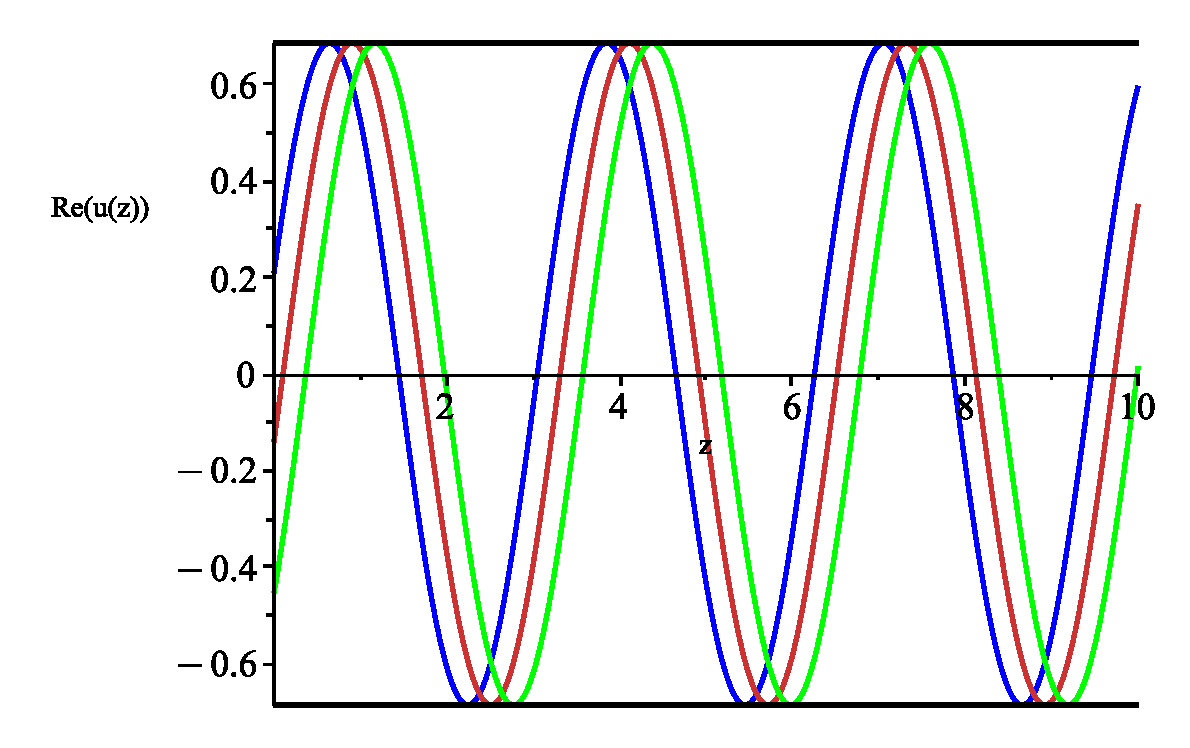
\includegraphics[width=\linewidth]{../graphics/Enveloppe/verlustlos/R0}
        \caption*{$r=0$, $t=0.1$ (blau), $t=0.2$ (orange) und $t=0.3$ (grün)}
    \end{minipage}\hfill
    \begin{minipage}{0.45\textwidth}
        \centering
        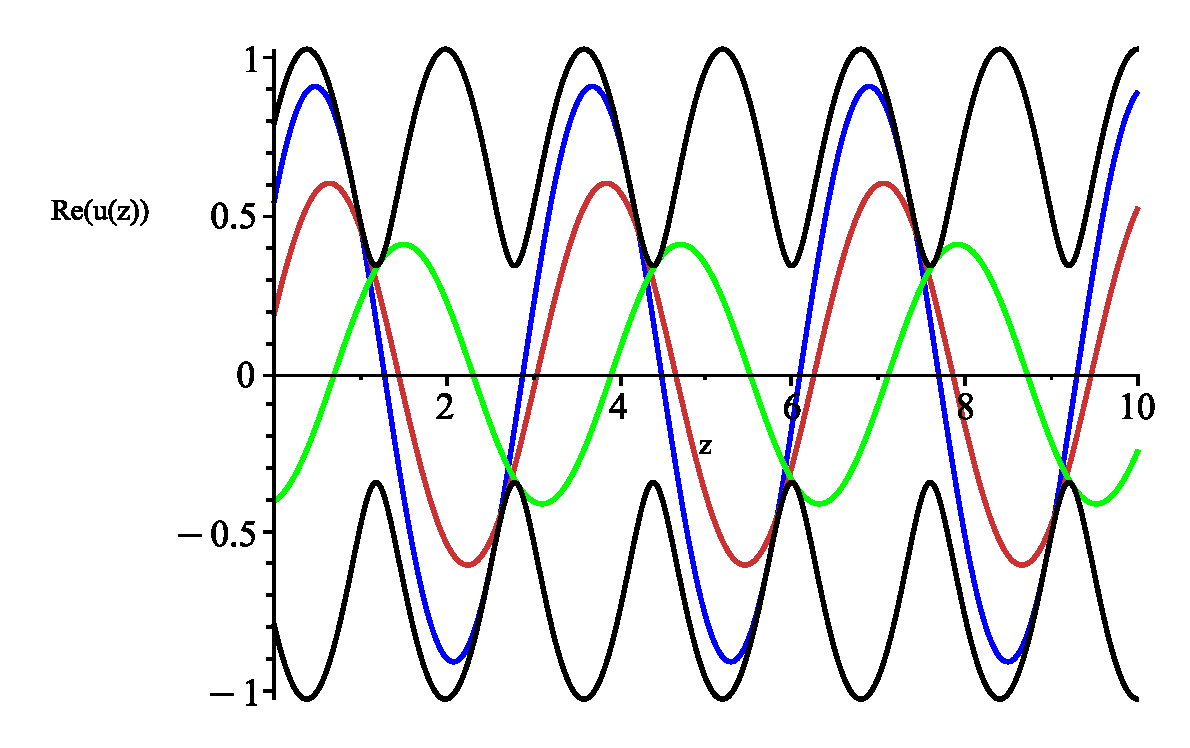
\includegraphics[width=\linewidth]{../graphics/Enveloppe/verlustlos/R0.5}
        \caption*{$r=0.5$, $t=0.1$ (blau), $t=0.2$ (orange) und $t=0.35$ (grün)}
    \end{minipage}

    \vspace{1ex}

    \begin{minipage}{0.45\textwidth}
        \centering
        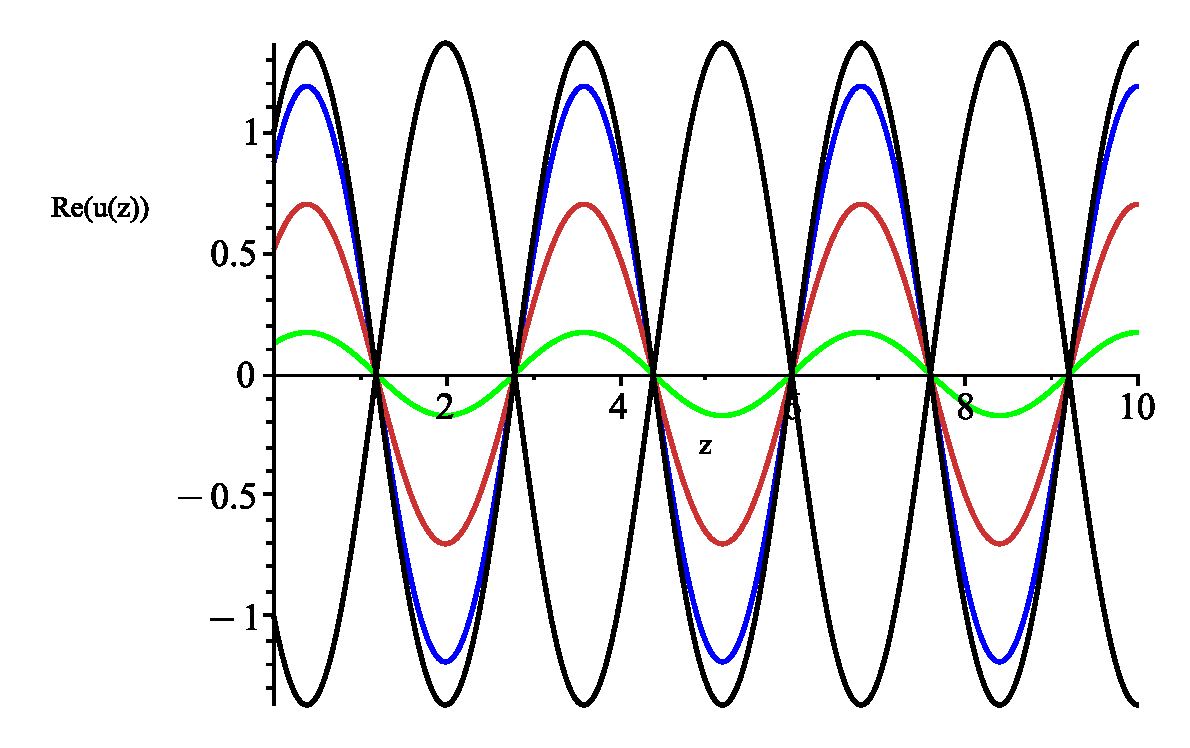
\includegraphics[width=\linewidth]{../graphics/Enveloppe/verlustlos/R1}
        \caption*{$r=1$, $t=0.1$ (blau), $t=0.2$ (orange) und $t=0.28$ (grün)}
    \end{minipage}\hfill
    \begin{minipage}{0.45\textwidth}
        \centering
        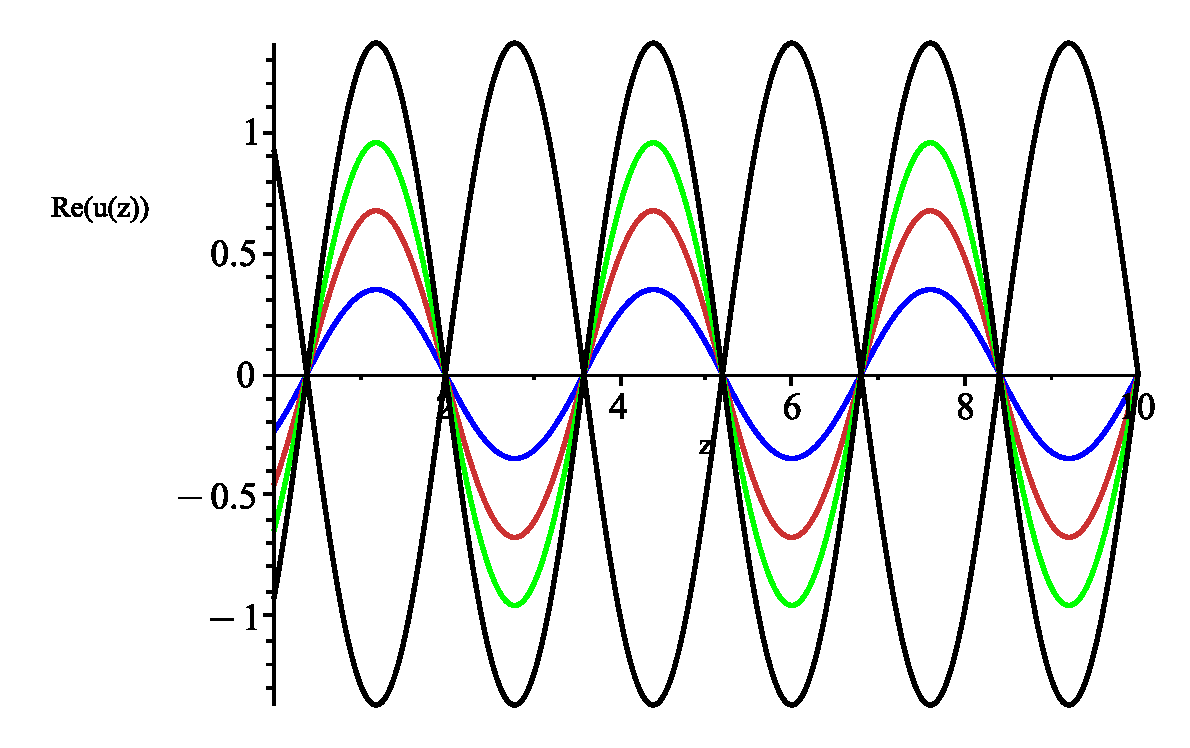
\includegraphics[width=\linewidth]{../graphics/Enveloppe/verlustlos/R-1}
        \caption*{$r=-1$, $t=0.05$ (blau), $t=0.1$ (orange) und $t=0.15$ (grün)}
    \end{minipage}

\end{figure}


\chapter{Wellenausbreitungen für den verlustbehafteten Fall}
Die folgende Abbildung zeigt die zeitliche Wellenausbreitung für verschiedene Zeiten $t$ und Reflexionskoeffizienten
$r$ entlang eines zylindrischen, verlustbehafteten Leiters (\mbox{$R^{\prime} \neq 0$}, $G^{\prime} \neq 0$). Die
schwarzen
Hüllkurven sind jeweils durch \[
\mathrm{Re} ( \left| U_{h}(z) + U_{r}(z) \right| )
\] bzw. \[
- \mathrm{Re} ( \left| U_{h}(z) + U_{r}(z) \right| )
\] gegeben. Die Maxima der Amplituden laufen auf der oberen, die Minima auf der unteren Hüllkurve für alle $t$.
\begin{figure}[!htpb]
    \begin{minipage}{0.45\textwidth}
        \centering
        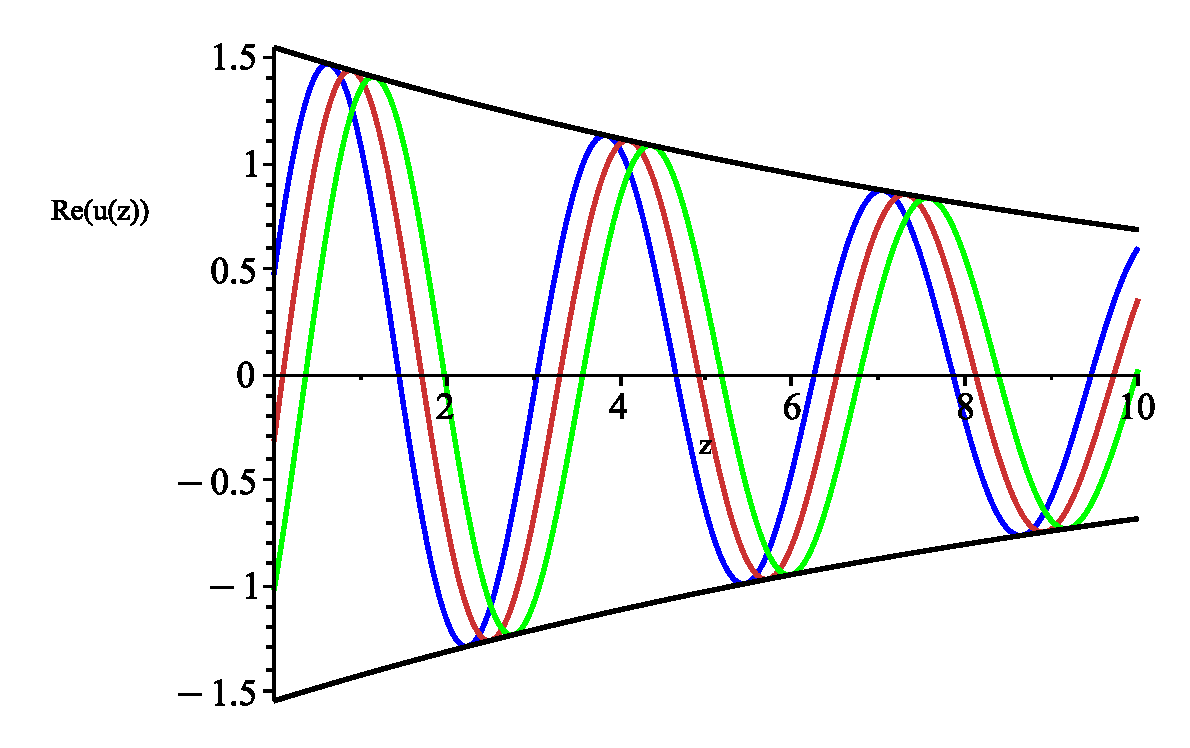
\includegraphics[width=\linewidth]{../graphics/Enveloppe/verlustbehaftet/R0}
        \caption*{$r=0$, $t=0.1$ (blau), $t=0.2$ (orange) und $t=0.3$ (grün)}
    \end{minipage}\hfill
    \begin{minipage}{0.45\textwidth}
        \centering
        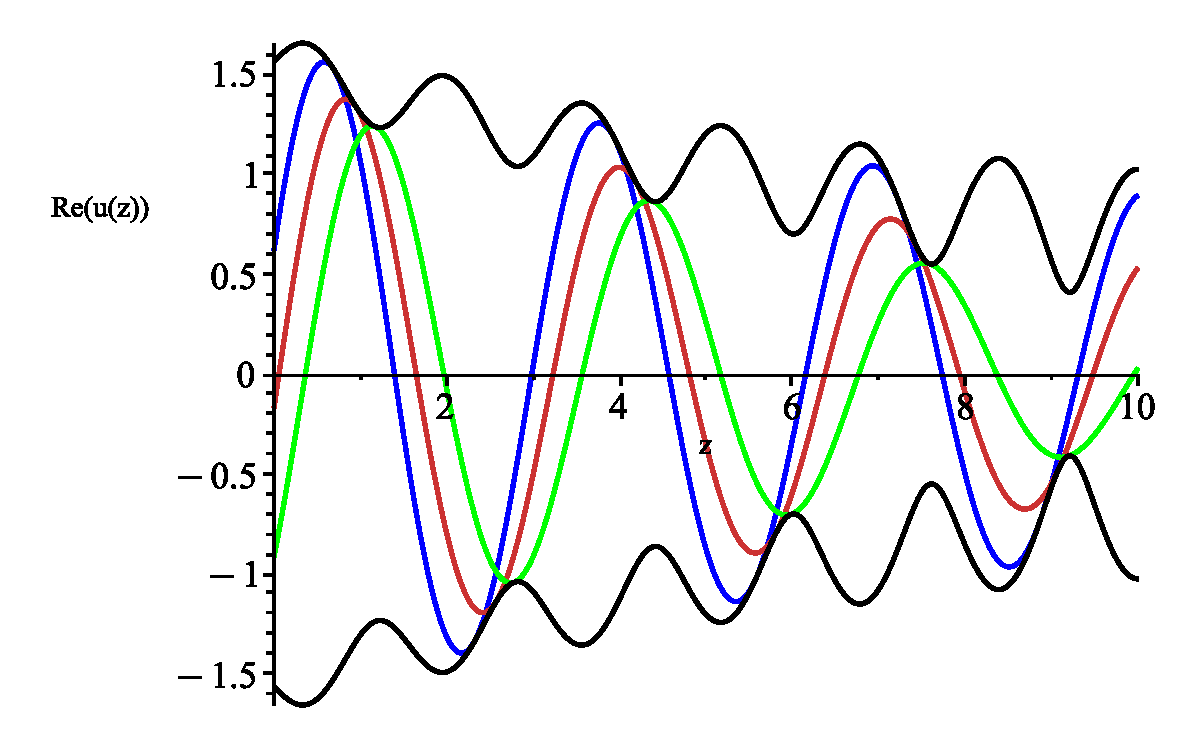
\includegraphics[width=\linewidth]{../graphics/Enveloppe/verlustbehaftet/R0.5}
        \caption*{$r=0.5$, $t=0.1$ (blau), $t=0.2$ (orange) und $t=0.3$ (grün)}
    \end{minipage}

    \vspace{1ex}

    \begin{minipage}{0.45\textwidth}
        \centering
        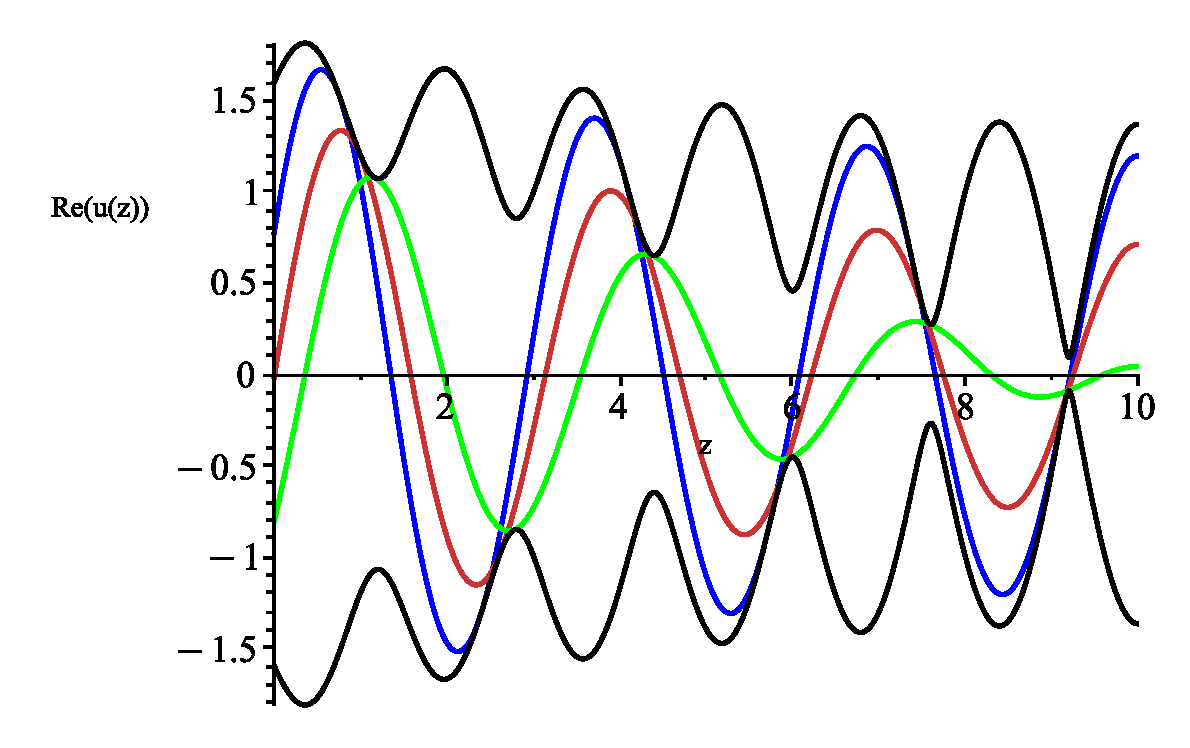
\includegraphics[width=\linewidth]{../graphics/Enveloppe/verlustbehaftet/R1}
        \caption*{$r=1$, $t=0.1$ (blau), $t=0.2$ (orange) und $t=0.3$ (grün)}
    \end{minipage}\hfill
    \begin{minipage}{0.45\textwidth}
        \centering
        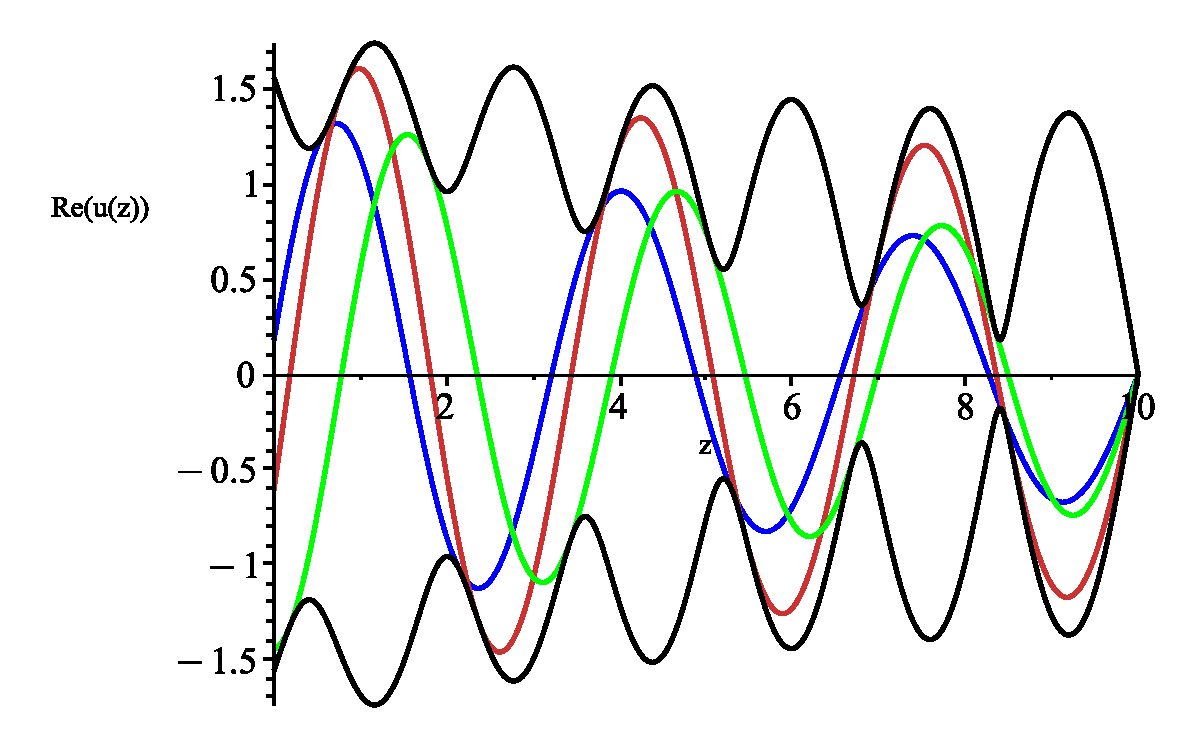
\includegraphics[width=\linewidth]{../graphics/Enveloppe/verlustbehaftet/R-1}
        \caption*{$r=-1$, $t=0.1$ (blau), $t=0.2$ (orange) und $t=0.5$ (grün)}
    \end{minipage}
\end{figure}


\printbibliography

\end{document}